\documentclass[12pt]{book}
\usepackage[T1]{fontenc}
\usepackage{times}
\usepackage{listings}
\usepackage{graphicx}
\usepackage{xcolor}
\usepackage{url}
% \usepackage{showidx}
\usepackage{imakeidx}
\usepackage{booktabs}
\usepackage{url}
\usepackage{etoolbox}  % for showidx
\usepackage{fullpage}
\usepackage{soul}
\usepackage[utf8]{inputenc}

\usepackage[hidelinks]{hyperref}  % should be last

% One space after periods
\frenchspacing

\hypersetup{pdfauthor={Russ Cox, Frans Kaashoek, Robert Morris},
            pdftitle={xv6: a simple, Unix-like teaching operating system},}
  
\lstset{basicstyle=\small\ttfamily}
\lstset{morecomment=[is]{[[[}{]]]}}
\lstset{escapeinside={(*@}{@*)}}
\lstset{xleftmargin=5.0ex}

\newcommand{\github}{https://github.com/mit-pdos/xv6-riscv/blob/riscv/}

\newcommand{\fileref}[1]{\href{\github/#1}{\small{(#1)}}}
\newcommand{\lineref}[2]{\href{\github/#1\#L#2}{\small{(#1:#2)}}}
\newcommand{\linerefs}[3]{\href{\github/#1\#L#2-L#3}{\small(#1:#2-#3)}}

\newcommand{\indextext}[1]{\textit{#1}\index{#1}}
\newcommand{\indextextx}[1]{{#1}\index{#1}}
\newcommand{\indexcode}[1]{\lstinline{#1}\index{#1@\lstinline{#1}}}

%% editing markup
\newcommand{\insertnote}[3]{\noindent\textcolor{#1}{\textbf{#2:} #3}}
\newcommand{\note}[1]{\insertnote{blue}{NOTE}{#1}}
\newcommand{\rtm}[1]{\insertnote{red}{RTM}{#1}}
\newcommand{\mfk}[1]{\insertnote{red}{MFK}{#1}}
%% for publishing book without notes
%\renewcommand{\insertnote}[3]{}

\title{\textbf{xv6: a simple, Unix-like teaching operating system}}
\author{Russ Cox \and Frans Kaashoek \and Robert Morris}

\makeindex

\begin{document}

\maketitle

\tableofcontents

\chapter*{Foreword and acknowledgments}


This is a draft text intended for a class on operating systems. It
explains the main concepts of operating systems by studying an example
kernel, named xv6.  Xv6 is modeled on Dennis Ritchie's and
Ken Thompson's Unix Version 6 (v6)~\cite{unix}.  Xv6 loosely follows the structure
and style of v6, but is implemented in ANSI C~\cite{kernighan} for 
a multi-core RISC-V~\cite{riscv}.

This text should be read along with the source code for xv6, an approach 
inspired by John Lions' Commentary on UNIX 6th Edition~\cite{lions}. See
\url{https://pdos.csail.mit.edu/6.1810} for pointers to on-line
resources for v6 and xv6, including several lab assignments
using xv6.

We have used this text in 6.828 and 6.1810, the operating system
classes at MIT.  We thank the faculty, teaching assistants, and
students of those classes who have all directly or indirectly
contributed to xv6.  In particular, we would like to thank Adam Belay,
Austin Clements, and Nickolai Zeldovich.  Finally, we would like to
thank people who emailed us bugs in the text or suggestions for
improvements: Abutalib Aghayev, Sebastian Boehm, brandb97, Anton
Burtsev, Raphael Carvalho, Tej Chajed,Brendan Davidson, Rasit
Eskicioglu, Color Fuzzy, Wojciech Gac, Giuseppe, Tao Guo, Haibo Hao,
Naoki Hayama, Chris Henderson, Robert Hilderman, Eden Hochbaum,
Wolfgang Keller, Paweł Kraszewski, Henry Laih, Jin Li, Austin Liew,
lyazj@github.com, Pavan Maddamsetti, Jacek Masiulaniec, Michael
McConville, m3hm00d, miguelgvieira, Mark Morrissey, Muhammed Mourad,
Harry Pan, Harry Porter, Siyuan Qian, Zhefeng Qiao, Askar Safin,
Salman Shah, Huang Sha, Vikram Shenoy, Adeodato Simó, Ruslan
Savchenko, Pawel Szczurko, Warren Toomey, tyfkda, tzerbib, Vanush
Vaswani, Xi Wang, and Zou Chang Wei, Sam Whitlock, Qiongsi Wu,
LucyShawYang, ykf1114@gmail.com, and Meng Zhou

If you spot errors or have suggestions for improvement, please send email to
Frans Kaashoek and Robert Morris (kaashoek,rtm@csail.mit.edu).

\chapter{Operating system interfaces}
\label{CH:UNIX}

The job of an operating system is to share a computer among
multiple programs and to provide a more useful set of services
than the hardware alone supports.
An operating system manages and abstracts
the low-level hardware, so that, for example,
a word processor need not concern itself with which type
of disk hardware is being used.
An operating system shares the hardware among multiple programs so
that they run (or appear to run) at the same time.
Finally, operating systems provide controlled ways for programs
to interact, so that they can share data or work together.

An operating system provides services to user programs through an interface.
\index{interface design}
Designing a good interface turns out to be
difficult.  On the one hand, we would like the interface to be
simple and narrow because that makes it easier to get the
implementation right.  On the other hand,
we may be tempted to offer many sophisticated features to applications.
The trick in
resolving this tension is to design interfaces that rely on a few
mechanisms that can be combined to provide much generality.

This book uses a single operating system as a concrete example to
illustrate operating system concepts.  That operating system,
xv6, provides the basic interfaces introduced by Ken Thompson and
Dennis Ritchie's Unix operating system~\cite{unix}, as well as mimicking Unix's
internal design.  Unix provides a
narrow interface whose mechanisms combine well, offering a surprising
degree of generality.  This interface has been so successful that
modern operating systems—BSD, Linux, macOS, Solaris, and even, to a
lesser extent, Microsoft Windows—have Unix-like interfaces.
Understanding xv6 is a good start toward understanding any of these
systems and many others.

As 
Figure~\ref{fig:os} shows,
xv6 takes the traditional form of a
\indextext{kernel},
a special program that provides
services to running programs.
Each running program, called a
\indextext{process},
has memory containing instructions, data, and a stack. The
instructions implement the
program's computation.  The data are the variables on which
the computation acts. The stack organizes the program's procedure calls.
A given computer typically has many processes but only a single
kernel.

When a
process needs to invoke a kernel service, it invokes 
a \indextext{system call},
one of the calls
in the operating system's interface.
The system call enters the kernel;
the kernel performs the service and returns.
Thus a process alternates between executing in
\indextext{user space}
and
\indextext{kernel space}.

As described in detail in subsequent chapters, the kernel uses the hardware protection mechanisms provided by a
CPU\footnote{
This text generally refers to the hardware element that executes a
computation with the term \indextext{CPU}, an acronym for central
processing unit.  Other documentation (e.g., the RISC-V specification)
also uses the words processor, core, and hart instead of CPU.
}
to
ensure that each process executing in user space can access only
its own memory.
The kernel executes with the hardware privileges required to
implement these protections; user programs execute without
those privileges.
When a user program invokes a system call, the hardware
raises the privilege level and starts executing a pre-arranged
function in the kernel.

\begin{figure}[t]
\center
\includegraphics[scale=0.5]{fig/os.pdf}
\caption{A kernel and two user processes.}
\label{fig:os}
\end{figure}

The collection of system calls that a kernel provides
is the interface that user programs see.
The xv6 kernel provides a subset of the services and system calls
that Unix kernels traditionally offer.  
Figure~\ref{fig:api} 
lists all of xv6's system calls.

The rest of this chapter outlines xv6's services---processes, memory,
file descriptors, pipes, and a file system---and illustrates them with
code snippets and discussions of how the \indextext{shell}, 
Unix's command-line user interface, uses
them. The shell's use of system calls illustrates how carefully they
have been designed.

The shell is an ordinary program that reads commands from the user
and executes them.
The fact that the shell is a user program, and not part of the kernel,
illustrates the power of the system call interface: there is nothing
special about the shell.
It also means that the shell is easy to replace; as a result,
modern Unix systems have a variety of
shells to choose from, each with its own user interface
and scripting features.
The xv6 shell is a simple implementation of the essence of
the Unix Bourne shell.  Its implementation can be found at 
\lineref{user/sh.c:1}.
%% 
%% 	Processes and memory
%% 
\section{Processes and memory}

An xv6 process consists of user-space memory (instructions, data, and stack)
and per-process state private to the kernel.
Xv6 
\indextext{time-share}s
processes: it transparently switches the available CPUs
among the set of processes waiting to execute.
When a process is not executing, xv6 saves the process's CPU registers,
restoring them when it next runs the process.
The kernel associates a process identifier, or
\indexcode{PID},
with each process.

\begin{figure}[t]
\center
\begin{tabular}{ll}
{\bf System call} & {\bf Description} \\
\midrule
int fork() & Create a process, return child's PID. \\
int exit(int status) & Terminate the current process; status reported to wait(). No return. \\
int wait(int *status) & Wait for a child to exit; exit status in *status; returns child PID. \\
int kill(int pid) & Terminate process PID. Returns 0, or -1 for error. \\
int getpid() & Return the current process's PID. \\
int sleep(int n) & Pause for n clock ticks. \\
int exec(char *file, char *argv[]) & Load a file and execute it with arguments; only returns if error. \\
char *sbrk(int n) & Grow process's memory by n bytes. Returns start of new memory. \\
int open(char *file, int flags) & Open a file; flags indicate read/write; returns an fd (file descriptor). \\
int write(int fd, char *buf, int n) & Write n bytes from buf to file descriptor fd; returns n. \\
int read(int fd, char *buf, int n) & Read n bytes into buf; returns number read; or 0 if end of file. \\
int close(int fd) & Release open file fd. \\
int dup(int fd) & Return a new file descriptor referring to the same file as fd.\\
int pipe(int p[]) & Create a pipe, put read/write file descriptors in p[0] and p[1]. \\
int chdir(char *dir) & Change the current directory. \\
int mkdir(char *dir) & Create a new directory. \\
int mknod(char *file, int, int) & Create a device file. \\
int fstat(int fd, struct stat *st) & Place info about an open file into *st. \\
int stat(char *file, struct stat *st) & Place info about a named file into *st. \\
int link(char *file1, char *file2) & Create another name (file2) for the file file1. \\
int unlink(char *file) & Remove a file. \\
\end{tabular}
\caption{Xv6 system calls. If not otherwise stated, these calls return
0 for no error, and -1 if there's an error.}
\label{fig:api}
\end{figure}

A process may create a new process using the
\indexcode{fork}
system call.
\lstinline{fork}
gives the new process an exact copy of the calling
process's user-space memory,
including instructions, data and stack.
\lstinline{fork}
returns in both the original and new processes.
In the original process, \lstinline{fork} returns the new process's
PID.
In the new process, \lstinline{fork} returns zero.
The original and new processes are often called the
\indextext{parent}
and
\indextext{child}.

For example, consider the following program fragment written in the C
programming language~\cite{kernighan}:
\begin{lstlisting}[]
int pid = fork();
if(pid > 0){
  printf("parent: child=%d\n", pid);
  pid = wait((int *) 0);
  printf("child %d is done\n", pid);
} else if(pid == 0){
  printf("child: exiting\n");
  exit(0);
} else {
  printf("fork error\n");
}
\end{lstlisting}
The
\indexcode{exit}
system call causes the calling process to stop executing and
to release resources such as memory and open files.
Exit takes an integer status argument,
conventionally 0 to indicate success and 1 to indicate failure.
The
\indexcode{wait}
system call returns the PID of an exited (or killed) child of the
current process and copies the exit status of the child to the address
passed to wait; if none of the caller's children
has exited,
\indexcode{wait}
waits for one to do so.
If the caller has no children, \lstinline{wait} immediately
returns -1.
If the parent doesn't care about the exit status of a child, it can
pass a 0 address to
\lstinline{wait}.

In the example, the output lines
\begin{lstlisting}[]
parent: child=1234
child: exiting
\end{lstlisting}
might come out in either order (or even intermixed), depending on whether the
parent or child gets to its
\indexcode{printf}
call first.
After the child exits, the parent's
\indexcode{wait}
returns, causing the parent to print
\begin{lstlisting}[]
parent: child 1234 is done
\end{lstlisting}
Although the child has the same memory contents as the parent initially, the
parent and child are executing with separate memory and separate registers:
changing a variable in one does not affect the other. For example, when the
return value of
\lstinline{wait}
is stored into
\lstinline{pid} 
in the parent process,
it doesn't change the variable 
\lstinline{pid}
in the child.  The value of
\lstinline{pid}
in the child will still be zero.

The
\indexcode{exec}
system call
replaces the calling process's memory with a new memory
image loaded from a file stored in the file system.
The file must have a particular format, which specifies which part of
the file holds instructions, which part is data, at which instruction
to start, etc. Xv6
uses the ELF format, which Chapter~\ref{CH:MEM} discusses in
more detail.
Usually the file is the result of compiling a program's source code.
When
\indexcode{exec}
succeeds, it does not return to the calling program;
instead, the instructions loaded from the file start
executing at the entry point declared in the ELF header.
\lstinline{exec}
takes two arguments: the name of the file containing the
executable and an array of string arguments.
For example:
\begin{lstlisting}[]
char *argv[3];

argv[0] = "echo";
argv[1] = "hello";
argv[2] = 0;
exec("/bin/echo", argv);
printf("exec error\n");
\end{lstlisting}
This fragment replaces the calling program with an instance
of the program 
\lstinline{/bin/echo}
running with the argument list
\lstinline{echo}
\lstinline{hello}.
Most programs ignore the first element of the argument array, which is 
conventionally the name of the program.

The xv6 shell uses the above calls to run programs on behalf of
users. The main structure of the shell is simple; see
\lstinline{main} 
\lineref{user/sh.c:/main/}.
The main loop reads a line of input from the user with
\indexcode{getcmd}.
Then it calls 
\lstinline{fork}, 
which creates a copy of the shell process. The
parent calls
\lstinline{wait},
while the child runs the command.  For example, if the user
had typed
``\lstinline{echo hello}''
to the shell,
\lstinline{runcmd}
would have been called with
``\lstinline{echo hello}''
as the argument.
\lstinline{runcmd} 
\lineref{user/sh.c:/runcmd/}
runs the actual command. For
``\lstinline{echo hello}'',
it would call
\lstinline{exec} 
\lineref{user/sh.c:/exec.ecmd/}.
If
\lstinline{exec}
succeeds then the child will execute instructions from
\lstinline{echo}
instead of
\lstinline{runcmd}.  
At some point
\lstinline{echo}
will call
\lstinline{exit},
which will cause the parent to return from
\lstinline{wait}
in 
\lstinline{main}
\lineref{user/sh.c:/main/}.

You might wonder why
\indexcode{fork}
and
\indexcode{exec}
are not combined in a single call; we will see later that 
the shell exploits the separation in its implementation of
I/O redirection.
To avoid the wastefulness of
creating a duplicate process and then immediately replacing it (with \lstinline{exec}),
operating kernels optimize the implementation of
\lstinline{fork}
for this use case by using virtual memory techniques such as
copy-on-write (see Section~\ref{sec:pagefaults}).

Xv6 allocates most user-space memory
implicitly:
\indexcode{fork}
allocates the memory required for the child's copy of the
parent's memory, and 
\indexcode{exec}
allocates enough memory to hold the executable file.
A process that needs more memory at run-time (perhaps for
\indexcode{malloc})
can call
\lstinline{sbrk(n)}
to grow its data memory by
\lstinline{n}
bytes;
\indexcode{sbrk}
returns the location of the new memory.

%% 
%% 	I/O and File descriptors
%% 
\section{I/O and File descriptors}

A 
\indextext{file descriptor} 
is a small integer representing a kernel-managed object
that a process may read from or write to.
A process may obtain a file descriptor by opening a file, directory,
or device, or by creating a pipe, or by duplicating an existing
descriptor.
For simplicity we'll often refer to the object a file descriptor
refers to as a ``file'';
the file descriptor interface abstracts away the differences between
files, pipes, and devices, making them all look like streams of bytes.
We'll refer to input and output as \indextext{I/O}.

Internally, the xv6 kernel uses the file descriptor
as an index into a per-process table,
so that every process has a private space of file descriptors
starting at zero.
By convention, a process reads from file descriptor 0 (standard input),
writes output to file descriptor 1 (standard output), and
writes error messages to file descriptor 2 (standard error).
As we will see, the shell exploits the convention to implement I/O redirection
and pipelines. The shell ensures that it always has three file descriptors
open
\lineref{user/sh.c:/open..console/},
which are by default file descriptors for the console.

The
\lstinline{read}
and
\lstinline{write}
system calls read bytes from and write bytes to
open files named by file descriptors.
The call
\lstinline{read(fd},
\lstinline{buf},
\lstinline{n)}
reads at most
\lstinline{n}
bytes from the file descriptor
\lstinline{fd},
copies them into
\lstinline{buf},
and returns the number of bytes read.
Each file descriptor that refers to a file
has an offset associated with it.
\lstinline{read}
reads data from the current file offset and then advances
that offset by the number of bytes read:
a subsequent
\lstinline{read}
will return the bytes following the ones returned by the first
\lstinline{read}.
When there are no more bytes to read,
\lstinline{read}
returns zero to indicate the end of the file.

The call
\lstinline{write(fd},
\lstinline{buf},
\lstinline{n)}
writes
\lstinline{n}
bytes from
\lstinline{buf}
to the file descriptor
\lstinline{fd}
and returns the number of bytes written.
Fewer than
\lstinline{n}
bytes are written only when an error occurs.
Like
\lstinline{read},
\lstinline{write}
writes data at the current file offset and then advances
that offset by the number of bytes written:
each
\lstinline{write}
picks up where the previous one left off.

The following program fragment (which forms the essence of the program
\lstinline{cat})
copies data from its standard input
to its standard output.  If an error occurs, it writes a message
to the standard error.
\begin{lstlisting}[]
char buf[512];
int n;

for(;;){
  n = read(0, buf, sizeof buf);
  if(n == 0)
    break;
  if(n < 0){
    fprintf(2, "read error\n");
    exit(1);
  }
  if(write(1, buf, n) != n){
    fprintf(2, "write error\n");
    exit(1);
  }
}
\end{lstlisting}
The important thing to note in the code fragment is that
\lstinline{cat}
doesn't know whether it is reading from a file, console, or a pipe.
Similarly 
\lstinline{cat}
doesn't know whether it is printing to a console, a file, or whatever.
The use of file descriptors and the convention that file descriptor 0
is input and file descriptor 1 is output allows a simple
implementation
of 
\lstinline{cat}.

The
\lstinline{close}
system call
releases a file descriptor, making it free for reuse by a future
\lstinline{open},
\lstinline{pipe},
or
\lstinline{dup}
system call (see below).
A newly allocated file descriptor 
is always the lowest-numbered unused
descriptor of the current process.

File descriptors and
\indexcode{fork}
interact to make I/O redirection easy to implement.
\lstinline{fork}
copies the parent's file descriptor table along with its memory,
so that the child starts with exactly the same open files as the parent.
The system call
\indexcode{exec}
replaces the calling process's memory but preserves its file table.
This behavior allows the shell to
implement \indextext{I/O redirection} by forking,
re-opening chosen file descriptors in the child,
and then calling \lstinline{exec} to run the new program.
Here is a simplified version of the code a shell runs for the
command
\lstinline{cat}
\lstinline{<}
\lstinline{input.txt}:
\begin{lstlisting}[]
char *argv[2];

argv[0] = "cat";
argv[1] = 0;
if(fork() == 0) {
  close(0);
  open("input.txt", O_RDONLY);
  exec("cat", argv);
}
\end{lstlisting}
After the child closes file descriptor 0,
\lstinline{open}
is guaranteed to use that file descriptor
for the newly opened
\lstinline{input.txt}:
0 will be the smallest available file descriptor.
\lstinline{cat}
then executes with file descriptor 0 (standard input) referring to
\lstinline{input.txt}.
The parent process's file descriptors are not changed by this
sequence, since it modifies only the child's descriptors.

The code for I/O redirection in the xv6 shell works in exactly this way
\lineref{user/sh.c:/case.REDIR/}.
Recall that at this point in the code the shell has already forked the
child shell and that 
\lstinline{runcmd} 
will call
\lstinline{exec}
to load the new program.

The second argument to \lstinline{open} consists of a set of
flags, expressed as bits, that control what \lstinline{open}
does. The possible values are defined in the file control (fcntl) header
\linerefs{kernel/fcntl.h:/RDONLY/,/TRUNC/}:
\lstinline{O_RDONLY},
\lstinline{O_WRONLY},
\lstinline{O_RDWR},
\lstinline{O_CREATE}, and
\lstinline{O_TRUNC},
which instruct \lstinline{open} to
open the file for reading,
or for writing,
or for both reading and writing,
to create the file if it doesn't exist,
and to truncate the file to zero length.

Now it should be clear why it is helpful that
\lstinline{fork}
and 
\lstinline{exec} 
are separate calls: between the two, the shell has a chance
to redirect the child's I/O without disturbing the I/O setup of the main shell.
One could instead imagine a hypothetical combined
\lstinline{forkexec} system call,
but the options for doing I/O redirection with such a call
seem awkward.
The shell could modify its own I/O
setup before calling \lstinline{forkexec} (and then
un-do those modifications); or
\lstinline{forkexec} could take instructions for I/O
redirection as arguments;
or (least attractively) every program like \lstinline{cat} could
be taught to do its own I/O redirection.

Although
\lstinline{fork}
copies the file descriptor table, each underlying file offset is shared
between parent and child.
Consider this example:
\begin{lstlisting}[]
if(fork() == 0) {
  write(1, "hello ", 6);
  exit(0);
} else {
  wait(0);
  write(1, "world\n", 6);
}
\end{lstlisting}
At the end of this fragment, the file attached to file descriptor 1
will contain the data
\lstinline{hello}
\lstinline{world}.
The
\lstinline{write}
in the parent
(which, thanks to
\lstinline{wait},
runs only after the child is done)
picks up where the child's
\lstinline{write}
left off.
This behavior helps produce sequential output from sequences
of shell commands, like
\lstinline{(echo}
\lstinline{hello};
\lstinline{echo}
\lstinline{world)}
\lstinline{>output.txt}.

The
\lstinline{dup}
system call duplicates an existing file descriptor,
returning a new one that refers to the same underlying I/O object.
Both file descriptors share an offset, just as the file descriptors
duplicated by
\lstinline{fork}
do.
This is another way to write
\lstinline{hello}
\lstinline{world}
into a file:
\begin{lstlisting}[]
fd = dup(1);
write(1, "hello ", 6);
write(fd, "world\n", 6);
\end{lstlisting}

Two file descriptors share an offset if they were derived from
the same original file descriptor by a sequence of
\lstinline{fork}
and
\lstinline{dup}
calls.
Otherwise file descriptors do not share offsets, even if they
resulted from 
\lstinline{open}
calls for the same file.  
\lstinline{dup} 
allows shells to implement commands like this:
\lstinline{ls}
\lstinline{existing-file}
\lstinline{non-existing-file}
\lstinline{>}
\lstinline{tmp1}
\lstinline{2>&1}.
The
\lstinline{2>&1}
tells the shell to give the command a file descriptor 2 that
is a duplicate of descriptor 1.
Both the name of the existing file and the error message for the
non-existing file will show up in the file
\lstinline{tmp1}.
The xv6 shell doesn't support I/O redirection for the error file
descriptor, but now you know how to implement it.

File descriptors are a powerful abstraction,
because they hide the details of what they are connected to:
a process writing to file descriptor 1 may be writing to a
file, to a device like the console, or to a pipe.
%% 
%% 	Pipes
%% 
\section{Pipes}

A 
\indextext{pipe} 
is a small kernel buffer exposed to processes as a pair of
file descriptors, one for reading and one for writing.
Writing data to one end of the pipe
makes that data available for reading from the other end of the pipe.
Pipes provide a way for processes to communicate.

The following example code runs the program
\lstinline{wc}
with standard input connected to
the read end of a pipe.
\begin{lstlisting}[]
int p[2];
char *argv[2];

argv[0] = "wc";
argv[1] = 0;

pipe(p);
if(fork() == 0) {
  close(0);
  dup(p[0]);
  close(p[0]);
  close(p[1]);
  exec("/bin/wc", argv);
} else {
  close(p[0]);
  write(p[1], "hello world\n", 12);
  close(p[1]);
}
\end{lstlisting}
The program calls
\lstinline{pipe},
which creates a new pipe and records the read and write
file descriptors in the array
\lstinline{p}.
After
\lstinline{fork},
both parent and child have file descriptors referring to the pipe.
The child calls \lstinline{close} and \lstinline{dup} to make file descriptor
zero refer to the read end of the pipe,
closes the file descriptors in
\lstinline{p},
and calls \lstinline{exec} to run
\lstinline{wc}.
When 
\lstinline{wc}
reads from its standard input, it reads from the pipe.
The parent closes the read side of the pipe,
writes to the pipe,
and then closes the write side.

If no data is available, a
\lstinline{read}
on a pipe waits for either data to be written or for all
file descriptors referring to the write end to be closed;
in the latter case,
\lstinline{read}
will return 0, just as if the end of a data file had been reached.
The fact that
\lstinline{read}
blocks until it is impossible for new data to arrive
is one reason that it's important for the child to
close the write end of the pipe
before executing
\lstinline{wc}
above: if one of
\lstinline{wc} 's
file descriptors referred to the write end of the pipe,
\lstinline{wc}
would never see end-of-file.

The xv6 shell implements pipelines such as
\lstinline{grep fork sh.c | wc -l}
in a manner similar to the above code
\lineref{user/sh.c:/case.PIPE/}.
The child process creates a pipe to connect the left end of the pipeline
with the right end. Then it calls
\lstinline{fork}
and
\lstinline{runcmd}
for the left end of the pipeline
and 
\lstinline{fork}
and
\lstinline{runcmd}
for the right end, and waits for both to finish.
The right end of the pipeline may be a command that itself includes a
pipe (e.g.,
\lstinline{a}
\lstinline{|}
\lstinline{b}
\lstinline{|}
\lstinline{c)}, 
which itself forks two new child processes (one for
\lstinline{b}
and one for
\lstinline{c}).
Thus, the shell may
create a tree of processes.  The leaves of this tree are commands and
the interior nodes are processes that wait until the left and right
children complete.

% In principle, one could have the interior nodes run the left end of a
% pipeline, but doing so correctly would complicate the
% implementation. Consider making just the following modification:
% change \lstinline{sh.c} to not fork for \lstinline{p->left} and run
% \lstinline{runcmd(p->left)} in the interior process. Then, for
% example, \lstinline{echo hi | wc} won't produce output, because when
% \lstinline{echo hi} exits in \lstinline{runcmd}, the interior process
% exits and never calls fork to run the right end of the pipe.  This
% incorrect behavior could be fixed by not calling \lstinline{exit} in
% \lstinline{runcmd} for interior processes, but this fix complicates
% the code: now \lstinline{runcmd} needs to know if it's in an interior
% process or not.  Complications also arise when not forking for
% \lstinline{runcmd(p->right)}.  For example, with just that
% modification, \lstinline{sleep 10 | echo hi} will immediately print
% ``hi' and a new prompt, instead of after 10 seconds; this happens because \lstinline{echo} runs
% immediately and exits, not waiting for \lstinline{sleep} to finish.
% Since the goal of the \lstinline{sh.c} is to be as simple as possible,
% it doesn't try to avoid creating interior processes.

Pipes may seem no more powerful than temporary files:
the pipeline
\begin{lstlisting}[]
echo hello world | wc
\end{lstlisting}
could be implemented without pipes as
\begin{lstlisting}[]
echo hello world >/tmp/xyz; wc </tmp/xyz
\end{lstlisting}
Pipes have at least three advantages over temporary files
in this situation.
First, pipes automatically clean themselves up;
with the file redirection, a shell would have to
be careful to remove
\lstinline{/tmp/xyz}
when done.
Second, pipes can pass arbitrarily long streams of
data, while file redirection requires enough free space
on disk to store all the data.
Third, pipes allow for parallel execution of pipeline stages,
while the file approach requires the first program to finish
before the second starts.
% Fourth, if you are implementing inter-process communication,
% pipes' blocking reads and writes are more efficient
% than the non-blocking semantics of files.
%% 
%% 	File system
%% 
\section{File system}

The xv6 file system provides data files,
which contain uninterpreted byte arrays,
and directories, which
contain named references to data files and other directories.
The directories form a tree, starting
at a special directory called the 
\indextext{root}.
A 
\indextext{path} 
like
\lstinline{/a/b/c}
refers to the file or directory named
\lstinline{c}
inside the directory named
\lstinline{b}
inside the directory named
\lstinline{a}
in the root directory
\lstinline{/}.
Paths that don't begin with
\lstinline{/}
are evaluated relative to the calling process's
\indextext{current directory},
which can be changed with the
\lstinline{chdir}
system call.
Both these code fragments open the same file
(assuming all the directories involved exist):
\begin{lstlisting}[]
chdir("/a");
chdir("b");
open("c", O_RDONLY);

open("/a/b/c", O_RDONLY);
\end{lstlisting}
The first fragment changes the process's current directory to
\lstinline{/a/b};
the second neither refers to nor changes the process's current directory.

There are system calls to create new files and directories:
\lstinline{mkdir}
creates a new directory,
\lstinline{open}
with the
\lstinline{O_CREATE}
flag creates a new data file,
and
\lstinline{mknod}
creates a new device file.
This example illustrates all three:
\begin{lstlisting}[]
mkdir("/dir");
fd = open("/dir/file", O_CREATE|O_WRONLY);
close(fd);
mknod("/console", 1, 1);
\end{lstlisting}
\lstinline{mknod}
creates a special file that refers to a device.
Associated with a device file are
the major and minor device numbers
(the two arguments to 
\lstinline{mknod}),
which uniquely identify a kernel device.
When a process later opens a device file, the kernel
diverts
\lstinline{read}
and
\lstinline{write}
system calls to the kernel device implementation
instead of passing them to the file system.

A file's name is distinct from the file itself;
the same underlying file, called an 
\indextext{inode}, 
can have multiple names,
called 
\indextext{links}.
Each link consists of an entry in a directory;
the entry contains a file name and a reference
to an inode.
An inode holds
\indextext{metadata}
about a file, including
its type (file or directory or device),
its length,
the location of the file's content on disk,
and the number of links to a file.

The
\lstinline{fstat}
system call
retrieves information from the inode that a
file descriptor refers to.
It fills in a
\lstinline{struct}
\lstinline{stat},
defined in
\lstinline{stat.h} \fileref{kernel/stat.h}
as:
\begin{lstlisting}[]
#define T_DIR     1   // Directory
#define T_FILE    2   // File
#define T_DEVICE  3   // Device

struct stat {
  int dev;     // File system's disk device
  uint ino;    // Inode number
  short type;  // Type of file
  short nlink; // Number of links to file
  uint64 size; // Size of file in bytes
};
\end{lstlisting}

The
\lstinline{link}
system call creates another file system name 
referring to the same inode as an existing file.
This fragment creates a new file named both
\lstinline{a}
and
\lstinline{b}.
\begin{lstlisting}[]
open("a", O_CREATE|O_WRONLY);
link("a", "b");
\end{lstlisting}
Reading from or writing to
\lstinline{a}
is the same as reading from or writing to
\lstinline{b}.
Each inode is identified by a unique
\textit{inode}
\textit{number}.
After the code sequence above, it is possible
to determine that
\lstinline{a}
and
\lstinline{b}
refer to the same underlying contents by inspecting the
result of 
\lstinline{fstat}:
both will return the same inode number 
(\lstinline{ino}),
and the
\lstinline{nlink}
count will be set to 2.

The
\lstinline{unlink}
system call removes a name from the file system.
The file's inode and the disk space holding its content
are only freed when the file's link count is zero and
no file descriptors refer to it.
Thus adding
\begin{lstlisting}[]
unlink("a");
\end{lstlisting}
to the last code sequence leaves the inode
and file content accessible as
\lstinline{b}.
Furthermore,
\begin{lstlisting}[]
fd = open("/tmp/xyz", O_CREATE|O_RDWR);
unlink("/tmp/xyz");
\end{lstlisting}
is an idiomatic way to create a temporary inode 
with no name
that will be cleaned up when the process closes 
\lstinline{fd}
or exits.

Unix provides
file utilities callable from the shell
as user-level programs, for example
\lstinline{mkdir},
\lstinline{ln},
and
\lstinline{rm}.
This design allows anyone to extend the command-line interface
by adding new user-level programs.  In hindsight this plan seems obvious,
but other systems designed at the time of Unix often built such commands into
the shell (and built the shell into the kernel).

One exception is
\lstinline{cd},
which is built into the shell
\lineref{user/sh.c:/if.buf.0..==..c./}.
\lstinline{cd}
must change the current working directory of the
shell itself.  If
\lstinline{cd}
were run as a regular command, then the shell would fork a child
process, the child process would run
\lstinline{cd},
and
\lstinline{cd}
would change the 
\textit{child} 's 
working directory.  The parent's (i.e.,
the shell's) working directory would not change.
%% 
%% 	Real world
%% 
\section{Real world}

Unix's combination of ``standard'' file
descriptors, pipes, and convenient shell syntax for
operations on them was a major advance in writing
general-purpose reusable programs.
The idea sparked a culture of ``software tools'' that was
responsible for much of Unix's power and popularity,
and the shell was the first so-called ``scripting language.''
The Unix system call interface persists today in systems like
BSD, Linux, and macOS.

The Unix system call interface has been standardized through the Portable
Operating System Interface (POSIX) standard.
Xv6 is
\textit{not}
POSIX compliant:  it is missing many system calls (including basic ones such as
\lstinline{lseek}),
and many of the system calls it does provide differ from the standard.
Our main goals for xv6 are
simplicity and clarity while providing a simple UNIX-like system-call interface.
Several people have extended xv6 with a few more system calls and a simple
C library in order to run basic Unix programs.  Modern kernels, however,
provide many more system calls, and many more kinds of kernel services, than
xv6.  For example, they support networking, windowing systems, user-level threads,
drivers for many devices, and so on.  Modern kernels evolve continuously and
rapidly, and offer many features beyond POSIX.

Unix unified access to multiple types of resources (files,
directories, and devices) with a single set of 
file-name and file-descriptor interfaces.
This idea can be extended to more kinds of resources;
a good example is Plan 9~\cite{Presotto91plan9},
which applied the ``resources are files''
concept to 
networks, graphics, and more.
However, most Unix-derived operating systems have
not followed this route.

The file system and file descriptors have been  powerful
abstractions.
Even so, there are other models for operating system interfaces.
Multics, a predecessor of Unix,
abstracted file storage in a way that made it look like memory,
producing a very different flavor of interface.
The complexity of the Multics design had a direct influence
on the designers of Unix, who aimed to build something simpler.
% XXX can we cut this, since its point is the same as the next paragraph?
% An operating system interface that went out of fashion
% decades ago but has recently returned is the idea of a virtual machine monitor.
% Such systems provide a superficially different interface from xv6,
% but the basic concepts are still the same:
% a virtual machine, like a process, consists of some memory and
% one or more register sets;
% the virtual machine has access to one large file called
% a virtual disk instead of a file system;
% virtual machines send messages to each other
% and the outside world using virtual network devices
% instead of pipes or files.

Xv6 does not provide a notion of users or of protecting
one user from another; in Unix terms, all xv6 processes
run as root.

This book examines how xv6 implements its Unix-like interface,
but the ideas and concepts apply to more than just Unix.
Any operating system must multiplex processes onto
the underlying hardware, isolate processes from each
other, and provide mechanisms for controlled
inter-process communication.
After studying xv6, you should be able to
look at other, more complex operating systems
and see the concepts underlying xv6 in those systems as well.

%% 
\section{Exercises}
%%

\begin{enumerate}

\item Write a program that uses UNIX system calls to
``ping-pong'' a byte between two processes over a pair
of pipes, one for each direction. Measure the
program's performance, in exchanges per second.

\end{enumerate}

%   terminology:
%     process: refers to execution in user space, or maybe struct proc &c
%     process memory: the lower part of the address space
%     process has one thread with two stacks (one for in kernel mode and one for
%     in user mode)
% talk a little about initial page table conditions:
%     paging not on, but virtual mostly mapped direct to physical,
%     which is what things look like when we turn paging on as well
%     since paging is turned on after we create first process.
%   mention why still have SEG_UCODE/SEG_UDATA?
%   do we ever really say what the low two bits of %cs do?
%     in particular their interaction with PTE_U
%   sidebar about why it is extern char[]

\chapter{Operating system organization}
\label{CH:FIRST}

A key requirement for an operating system is to support several activities at once.  For
example, using the system call interface described in
Chapter~\ref{CH:UNIX}
a process can start new processes with 
\lstinline{fork}.
The operating system must 
\indextext{time-share} 
the resources of the computer among these processes.
For example, even if there are more processes
than there are hardware CPUs, the operating
system must ensure that all of the processes
get a chance to execute.  The operating system must also arrange for
\indextext{isolation} 
between the processes.
That is, if one process has a bug and malfunctions,
it shouldn't affect processes that
don't depend on the buggy process.
Complete isolation, however, is too strong, since it should be possible for
processes to intentionally interact; pipelines are an example.
Thus
an operating system must fulfill three requirements: multiplexing, isolation,
and interaction.

This chapter provides an overview of how operating systems are
organized to achieve these three requirements.  It turns out there are
many ways to do so, but this text focuses on mainstream designs
centered around a \indextext{monolithic kernel}, which is used by many
Unix operating systems.  This chapter also provides an overview of an
xv6 process, which is the unit of isolation in xv6, and the
creation of the first process when xv6 starts.

Xv6 runs on a \indextext{multi-core}\footnote{
By ``multi-core'' this text means multiple CPUs that share memory but execute
in parallel, each with its own set of registers.
This text sometimes uses the term
\indextext{multiprocessor} as a synonym for multi-core,
though multiprocessor can also refer more specifically to a computer with
several distinct processor chips.} RISC-V microprocessor,
and much of its low-level
functionality (for example, its process implementation) is specific to
RISC-V.  RISC-V is a 64-bit CPU, and xv6 is written in ``LP64'' C,
which means long (L) and pointers (P) in the C programming language
are 64 bits, but an {\tt int} is 32 bits.  This book assumes the reader has done
a bit of machine-level programming on some architecture, and will
introduce RISC-V-specific ideas as they come up.
The user-level ISA~\cite{riscv:user} and privileged
architecture~\cite{riscv:priv} documents are the complete
specifications.
You may also refer to
``The RISC-V Reader: An Open Architecture
Atlas''~\cite{riscv}.

The CPU in a complete computer is surrounded by support hardware, much
of it in the form of I/O interfaces. Xv6 is written for the support
hardware simulated by qemu's ``-machine virt'' option. This includes
RAM, a ROM containing boot code, a serial connection to the user's
keyboard/screen, and a disk for storage.

%% 
\section{Abstracting physical resources}
%% 

The first question one might ask when encountering an operating system is why
have it at all?  That is, one could implement the system calls in
Figure~\ref{fig:api}
as a library, with which applications link.  In this plan,
each application could even have its own library tailored to its needs.
Applications could directly interact with hardware resources
and use those resources in the best way for the application (e.g., to achieve
high or predictable performance).  Some operating systems for
embedded devices or real-time systems are organized in this way.

The downside of this library approach is that, if there is more than one
application running, the applications must be well-behaved.
For example, each application must periodically give up the
CPU so that other applications can run.
Such a 
\textit{cooperative} 
time-sharing scheme may be OK if all applications trust each
other and have no bugs. It's more typical for applications
to not trust each other, and to have bugs, so one often wants
stronger isolation than a cooperative scheme provides.

To achieve strong isolation it's helpful to forbid applications from
directly accessing sensitive hardware resources, and instead to abstract the
resources into services.  For example, Unix applications interact with storage
only through the file system's
\lstinline{open},
\lstinline{read},
\lstinline{write}, 
and
\lstinline{close}
system calls,
instead of reading and writing the disk directly. 
This provides the application with the convenience of pathnames, and it allows
the operating system (as the implementer of the interface) to manage the disk. 
Even if isolation is not a concern,
programs that interact intentionally (or just wish to keep
out of each other's way) are likely to find a file system a more convenient
abstraction than direct use of the disk.

Similarly, Unix transparently switches hardware CPUs among processes,
saving and restoring register state as necessary,
so that applications don't have to be
aware of time-sharing.  This transparency allows the operating system to share
CPUs even if some applications are in infinite loops.

As another example, Unix processes use 
\lstinline{exec}
to build up their memory image, instead of directly interacting with physical
memory.  This allows the operating system to decide where to place a process in
memory; if memory is tight, the operating system might even store some of
a process's data on disk.
\lstinline{exec}
also provides
users with the convenience of a file system to store executable program images.  

Many forms of interaction among Unix processes occur via file descriptors.
Not only do file descriptors abstract away many details (e.g.,
where data in a pipe or file is stored), they are also defined in a
way that simplifies interaction.
For example, if one application in a pipeline fails, the kernel
generates an end-of-file signal for the next process in the pipeline.

The system-call interface in
Figure~\ref{fig:api}
is carefully designed to provide both programmer convenience and
the possibility of strong isolation.  The Unix interface
is not the only way to abstract resources, but it has proved to be a good
one.

%% 
\section{User mode, supervisor mode, and system calls}
%% 

Strong isolation requires a hard boundary between applications and the operating
system.  If the application makes a mistake, we don't want the operating system
to fail or other applications to fail. Instead, the operating system should be
able to clean up the failed application and continue running other applications.
To achieve strong isolation, the operating system must arrange that applications cannot modify (or even
read) the operating system's data structures and instructions and that
applications cannot access other processes' memory.

CPUs provide hardware support for strong isolation.   For
example, RISC-V has three modes in which
the CPU can execute instructions:
\indextext{machine mode},
\indextext{supervisor mode}, and
\indextext{user mode}.
Instructions executing in machine mode have full privilege; a
CPU starts in machine mode.  Machine mode is mostly intended for
setting up the computer during boot.  Xv6 executes a few lines in machine mode and
then changes to supervisor mode.

In supervisor mode the CPU is allowed to execute 
\indextext{privileged instructions}:
for example, enabling and disabling interrupts,  reading and writing
the register that holds the address of a page table, etc.
If an application in user mode attempts to execute
a privileged instruction, then the CPU doesn't execute the instruction, but switches
to supervisor mode so that supervisor-mode code can terminate the application,
because it did something it shouldn't be doing. 
Figure~\ref{fig:os}
in Chapter~\ref{CH:UNIX} illustrates this organization.  An application can
execute only user-mode instructions (e.g., adding numbers, etc.) and is said to
be running in 
\indextext{user space},
while the software in supervisor mode can also execute privileged instructions and
is said to be running in
\indextext{kernel space}.
The software running in kernel space (or in supervisor mode) is called
the
\indextext{kernel}.

An application that wants to invoke a kernel function (e.g., the
\lstinline{read}
system call in xv6) must 
transition to the kernel; an application \emph{cannot} invoke a kernel
function directly.  CPUs provide a special instruction that switches the
CPU from user mode to supervisor mode and enters the kernel at an entry point
specified by the kernel.  (RISC-V
provides the 
\indexcode{ecall}
instruction for this purpose.)  Once the CPU has switched to supervisor mode,
the kernel can then validate the arguments of the system call (e.g.,
check if the address passed to the system call is part of the application's memory), decide whether
the application is allowed to perform the requested operation (e.g.,
check if the application is allowed to write the specified file), and then deny it
or execute it.  It is important that the kernel control the entry point for
transitions to supervisor mode; if the application could decide the kernel entry
point, a malicious application could, for example, enter the kernel at a point where the
validation of arguments is skipped.

%% 
\section{Kernel organization}
%% 

A key design question is what part of the operating
system should run in supervisor mode. 
One possibility is that the entire operating system resides
in the kernel, so that the implementations of all system calls
run in supervisor mode.
This organization is called a
\indextext{monolithic kernel}.

In this organization the entire operating system consists of a single
program running with full hardware
privilege. This organization is convenient because the OS designer doesn't have
to decide which parts of the operating system don't need full hardware
privilege.  Furthermore, it is easier for different parts of the operating system to
cooperate.  For example, an operating system might have a buffer cache that can
be shared both by the file system and the virtual memory system. 

A downside of the monolithic organization is that the interactions among
different parts of the operating system are often complex (as we will see in the
rest of this text), and therefore it is easy for an operating system developer
to make a mistake.  In a monolithic kernel, a mistake is fatal, because an error
in supervisor mode will often cause the kernel to fail.  If the kernel fails,
the computer stops working, and thus all applications fail too.  The computer
must reboot to start again.

To reduce the risk of mistakes in the kernel, OS designers can minimize the
amount of operating system code that runs in supervisor mode, and execute the
bulk of the operating system in user mode.
This kernel organization is called a
\indextext{microkernel}.

\begin{figure}[t]
\center
\includegraphics[scale=0.5]{fig/mkernel.pdf}
\caption{A microkernel with a file-system server}
\label{fig:mkernel}
\end{figure}

Figure~\ref{fig:mkernel}
illustrates this microkernel design.  In the figure, the file system runs as a
user-level process.  OS services running as processes are called servers.
To allow applications to interact with the
file server, the kernel provides an inter-process communication
mechanism to send messages from one
user-mode process to another.  For example, if an application like the shell
wants to read or write a file, it sends a message to the file server and waits
for a response. 

In a microkernel, the kernel interface consists of a few low-level
functions for starting applications, sending messages,
accessing device hardware, etc.  This organization allows the kernel to be 
relatively simple, as most of the operating system
resides in user-level servers.

In the real world, both monolithic kernels and microkernels are
popular. Many
Unix kernels are monolithic. For example, Linux has a monolithic kernel,
although some OS functions run as user-level servers (e.g., the window
system).  Linux delivers high performance to OS-intensive applications, partially
because the subsystems of the kernel can be tightly integrated.

Operating systems such as Minix, L4, and QNX are organized as a microkernel with
servers, and have seen wide deployment in embedded settings.  A
variant of L4, seL4, is small enough that it has been verified for
memory safety and other security properties~\cite{sel4}.

There is much debate among developers of operating systems about which
organization is better, and there is no conclusive evidence one way or
the other.  Furthermore, it depends much on what ``better'' means:
faster performance, smaller code size, reliability of the kernel,
reliability of the complete operating system (including user-level
services), etc.

There are also practical considerations that may be more important
than the question of which organization.  Some operating systems
have a microkernel but run some of the user-level services in kernel
space for performance reasons.  Some operating systems have monolithic
kernels because that is how they started and there is little incentive
to move to a pure microkernel organization, because new features may
be more important than rewriting the existing operating system to fit a microkernel
design.

From this book's perspective, microkernel and monolithic operating
systems share many key ideas.  They implement system calls, they use
page tables, they handle interrupts, they support processes, they use
locks for concurrency control, they implement a file system,
etc. This book focuses on these core ideas.

Xv6 is
implemented as a monolithic kernel, like most Unix operating systems.
Thus, the xv6 kernel interface corresponds to the operating system
interface, and the kernel implements the complete operating system.  Since 
xv6 doesn't provide many services, its kernel is smaller than some
microkernels, but conceptually xv6 is monolithic.  

\section{Code: xv6 organization}

\begin{figure}[t]
\center
\begin{tabular}{l|l}
{\bf File} & {\bf Description} \\
\midrule
bio.c & Disk block cache for the file system. \\
console.c & Connect to the user keyboard and screen. \\
entry.S & Very first boot instructions. \\
exec.c & exec() system call. \\
file.c & File descriptor support. \\
fs.c & File system. \\
kalloc.c & Physical page allocator. \\
kernelvec.S & Handle traps from kernel. \\
log.c & File system logging and crash recovery. \\
main.c & Control initialization of other modules during boot. \\
pipe.c & Pipes. \\
plic.c & RISC-V interrupt controller. \\
printf.c & Formatted output to the console. \\
proc.c & Processes and scheduling. \\
sleeplock.c & Locks that yield the CPU. \\
spinlock.c & Locks that don't yield the CPU. \\
start.c & Early machine-mode boot code. \\
string.c & C string and byte-array library. \\
swtch.S & Thread switching. \\
syscall.c & Dispatch system calls to handling function. \\
sysfile.c & File-related system calls. \\
sysproc.c & Process-related system calls. \\
trampoline.S & Assembly code to switch between user and kernel. \\
trap.c & C code to handle and return from traps and interrupts. \\
uart.c & Serial-port console device driver. \\
virtio\_disk.c & Disk device driver. \\
vm.c & Manage page tables and address spaces. \\
\end{tabular}
\caption{Xv6 kernel source files.}
\label{fig:source}
\end{figure}

The xv6 kernel source is in the {\tt kernel/} sub-directory. The
source is divided into files, following a rough notion of modularity;
Figure~\ref{fig:source} lists the files.  The inter-module interfaces
are defined in \lstinline{defs.h} \fileref{kernel/defs.h}.

%% 
\section{Process overview}
%% 

The unit of isolation in xv6 (as in other Unix operating systems) is a 
\indextext{process}.
The process abstraction prevents one process from wrecking or spying on
another process's memory, CPU, file descriptors, etc.  It also prevents a process
from wrecking the kernel itself, so that a process can't subvert the kernel's
isolation mechanisms.
The kernel must implement the process abstraction with care because
a buggy or malicious application may trick the kernel or hardware into doing
something bad (e.g., circumventing isolation).  The mechanisms used by
the kernel to implement processes include the user/supervisor mode flag, address spaces,
and time-slicing of threads.

To help enforce isolation, the process abstraction provides the
illusion to a program that it has its own private machine.  A process provides
a program with what appears to be a private memory system, or
\indextext{address space}, 
which other processes cannot read or write.
A process also provides the program with what appears to be its own
CPU to execute the program's instructions.

Xv6 uses page tables (which are implemented by hardware) to give each process
its own address space. The RISC-V page table
translates (or ``maps'') a
\indextext{virtual address}
(the address that an RISC-V instruction manipulates) to a
\indextext{physical address}
(an address that the CPU sends to main memory).

\begin{figure}[t]
\centering
\includegraphics[scale=0.5]{fig/as.pdf}
\caption{Layout of a process's virtual address space}
\label{fig:as}
\end{figure}

Xv6 maintains a separate page table for each process that defines that process's
address space. As illustrated in 
Figure~\ref{fig:as},
an address space includes the process's
\indextext{user memory}
starting at virtual address zero. Instructions come first,
followed by global variables, then the stack,
and finally a ``heap'' area (for malloc)
that the process can expand as needed.
There are a number of factors that limit the
maximum size of a process's address space:
pointers on the RISC-V are 64 bits wide;
the hardware uses only the low 39 bits when
looking up virtual addresses in page tables;
and xv6 uses only 38 of those 39 bits.
Thus, the maximum address is $2^{38}-1$ =
0x3fffffffff, which is \lstinline{MAXVA}~\lineref{kernel/riscv.h:/define.MAXVA/}.
At the top of the address space xv6 places
a \indextext{trampoline} page (4096 bytes)
and a \indextext{trapframe} page.  Xv6 uses these two pages
to transition into the kernel and back;
the trampoline page contains the code to transition in and out
of the kernel, and the trapframe is where the kernel saves
the process's user registers,
as Chapter~\ref{CH:TRAP} explains.

The xv6 kernel maintains many pieces of state for each process,
which it gathers into a
\indexcode{struct proc}
\lineref{kernel/proc.h:/^struct.proc/}.
A process's most important pieces of kernel state are its 
page table, its kernel stack, and its run state.
We'll use the notation
\indexcode{p->xxx}
to refer to elements of the
\lstinline{proc}
structure; for example,
\indexcode{p->pagetable} is a pointer to the process's page table.

Each process has a thread of control (or 
\indextext{thread}
for short) that holds the state needed to execute the process.
At any given time, a thread might be executing on a CPU,
or suspended (not executing, but capable of resuming executing
in the future).
To switch a CPU between processes,
the kernel suspends the thread currently running on that CPU
and saves its state,
and restores the state of another process's previously-suspended
thread.  Much of the state of a thread (local variables, function call return
addresses) is stored on the thread's stacks.
Each process has two stacks: a user stack and a kernel stack
(\indexcode{p->kstack}).
When the process is executing user instructions, only its user stack
is in use, and its kernel stack is empty.
When the process enters the kernel (for a system call or interrupt),
the kernel code executes on the process's kernel stack; while
a process is in the kernel, its user stack still contains saved
data, but isn't actively used.
A process's thread alternates between actively using its user stack
and its kernel stack. The kernel stack is separate (and protected from
user code) so that the kernel
can execute even if a process has wrecked its user stack.

A process can make a system call by executing the RISC-V \indexcode{ecall}
instruction. This instruction raises the hardware privilege level and
changes the program counter to a kernel-defined entry point.  The code
at the entry point switches to the process's kernel stack and executes the kernel
instructions that implement the system call.  When the system call
completes, the kernel switches back to the user stack and returns to
user space by calling the \indexcode{sret} instruction, which lowers
the hardware privilege level and resumes executing user instructions
just after the system call instruction.  A process's thread can
``block'' in the kernel to wait for I/O, and resume where it left off
when the I/O has finished.

\indexcode{p->state} 
indicates whether the process is allocated, ready
to run, currently running on a CPU, waiting for I/O, or exiting.

\indexcode{p->pagetable}
holds the process's page table, in the format
that the RISC-V hardware expects.
Xv6 causes the paging hardware to use a process's
\lstinline{p->pagetable}
when executing that process in user space.
A process's page table also serves as the record of the
addresses of the physical pages allocated to store the process's
memory.

In summary, a process bundles two design ideas: an address space to
give a process the illusion of its own memory, and a thread to give
the process the illusion of its own CPU.  In xv6, a process consists
of one address space and one thread.  In real operating systems a
process may have more than one thread to take advantage of multiple CPUs.

%% 
\section{Code: starting xv6, the first process and system call}
%% 
To make xv6 more concrete, we'll outline how the kernel starts and
runs the first process. The subsequent chapters will describe the
mechanisms that show up in this overview in more detail.

When the RISC-V computer powers on, it initializes
itself and runs a boot loader which is stored in read-only
memory.  The boot loader loads the xv6 kernel into memory.  Then, in
machine mode, the CPU executes xv6 starting at
\indexcode{_entry}
\lineref{kernel/entry.S:/^.entry:/}.
The RISC-V starts with paging hardware disabled:
virtual addresses map directly to physical addresses.

The loader loads the xv6 kernel into memory at physical address
\texttt{0x80000000}.
The reason it places the kernel at
\texttt{0x80000000}
rather than
\texttt{0x0}
is because the address range
\texttt{0x0:0x80000000}
contains I/O devices.

The instructions at
\lstinline{_entry}
set up a stack so that xv6 can run C code.
Xv6 declares space for an initial stack,
\lstinline{stack0},
in the file
\lstinline{start.c}
\lineref{kernel/start.c:/stack0/}.
The code at
\lstinline{_entry}
loads the stack pointer register
\texttt{sp}
with the address
\lstinline{stack0+4096},
the top of the stack, because the stack
on RISC-V grows down.
Now that the kernel has a stack,
\lstinline{_entry}
calls into C code at
\lstinline{start}
\lineref{kernel/start.c:/^start/}.

The function
\lstinline{start}
performs some configuration that is only allowed in
machine mode, and then switches to supervisor mode.
To enter supervisor mode, RISC-V
provides the instruction
\lstinline{mret}.
This instruction is most often used to return from
a previous call from supervisor mode to machine mode.
\lstinline{start} isn't returning from such a call, but
sets things up as if it were:
it sets the previous privilege mode to
supervisor in the register
\lstinline{mstatus},
it sets the return address to
\lstinline{main}
by writing
\lstinline{main}'s
address into
the register
\lstinline{mepc},
disables virtual address translation in supervisor mode
by writing
\lstinline{0}
into the page-table register
\lstinline{satp},
and delegates all interrupts and exceptions
to supervisor mode.

Before jumping into supervisor mode,
\lstinline{start}
performs one more task: it programs the clock
chip to generate timer interrupts.
With this housekeeping out of the way,
\lstinline{start}
``returns'' to supervisor
mode by calling
\lstinline{mret}.
This causes the program counter to change
to
\lstinline{main}
\lineref{kernel/main.c:/^main/},
the address previously stored in \lstinline{mepc}.

After
\lstinline{main}
\lineref{kernel/main.c:/^main/}  
initializes several devices and subsystems, 
it creates the first process by calling 
\lstinline{userinit}
\lineref{kernel/proc.c:/^userinit/}.
The first process executes a small program written in RISC-V assembly,
which makes the first system call in xv6.
\indexcode{initcode.S} 
\lineref{user/initcode.S:3} loads the number for the \lstinline{exec}
system call, \lstinline{SYS_EXEC}
\lineref{kernel/syscall.h:/exec/},
into
register {\tt a7},
and then calls \lstinline{ecall} to re-enter the kernel.

The kernel uses the number in register {\tt a7} in \lstinline{syscall}
\lineref{kernel/syscall.c:/^syscall/} to call the desired system call.
The system call table \lineref{kernel/syscall.c:/syscalls/} maps
\lstinline{SYS_EXEC} to the function \lstinline{sys_exec}, which the kernel
invokes.  As we saw in Chapter~\ref{CH:UNIX}, \indexcode{exec}
replaces the memory and registers of the current process with a new
program (in this case, \indexcode{/init}).

Once the kernel has completed 
\lstinline{exec},
it returns to user space in
the \lstinline{/init} process.
\lstinline{init}
\lineref{user/init.c:/^main/}
creates a new console device file
if needed
and then opens it as file descriptors 0, 1, and 2.
Then it starts a shell on the console.
The system is up.

\section{Security Model}

You may wonder how the operating system deals with buggy or malicious
code. Because coping with malice is strictly harder than dealing with
accidental bugs, it's reasonable to 
focus mostly on providing security against malice.
Here's a high-level view of typical security assumptions and
goals in operating system design.

The operating system must assume that a process's user-level code will
do its best to wreck the kernel or other processes. User code may try
to dereference pointers outside its allowed address space; it may
attempt to execute any RISC-V instructions, even those not intended
for user code; it may try to read and write any RISC-V control
register; it may try to directly access device hardware;
and it may pass clever values to system calls in an attempt
to trick the kernel into crashing or doing something stupid. The
kernel's goal is to restrict each user processes so that all it can do is
read/write/execute its own user memory, use the 32 general-purpose
RISC-V registers, and affect the kernel and other processes in the
ways that system calls are intended to allow. The kernel must prevent
any other actions. This is typically an absolute requirement in kernel
design.

The expectations for the kernel's own code are quite different. Kernel
code is assumed to be written by well-meaning and careful programmers.
Kernel code is expected to be bug-free, and certainly to contain
nothing malicious. This assumption affects how we analyze kernel code.
For example, there are many internal kernel functions (e.g., the spin
locks) that would cause serious problems if kernel code used them
incorrectly. When examining any specific piece of kernel code, we'll
want to convince ourselves that it behaves correctly. We assume,
however, that kernel code in general is correctly written, and follows
all the rules about use of the kernel's own functions and data
structures. At the hardware level, the RISC-V CPU, RAM, disk, etc. are
assumed to operate as advertised in the documentation, with no
hardware bugs.

Of course in real life things are not so straightforward. It's
difficult to prevent clever user code from making a system unusable
(or causing it to panic) by consuming kernel-protected resources --
disk space, CPU time, process table slots, etc. It's usually
impossible to write bug-free kernel code or design bug-free hardware; if the
writers of malicious user code are aware of kernel or hardware bugs,
they will exploit them. Even in mature, widely-used kernels, such as
Linux, people discover new vulnerabilities
continuously~\cite{mitre:cves}. It's worthwhile to design safeguards into the
kernel against the possibility that it has bugs: assertions, type
checking, stack guard pages, etc. Finally, the distinction between
user and kernel code is sometimes blurred: some privileged user-level
processes may provide essential services and effectively be part of
the operating system, and in some operating systems privileged user
code can insert new code into the kernel (as with Linux's loadable
kernel modules).


%% 
\section{Real world}
%% 

Most operating systems have adopted the process concept, and most
processes look similar to xv6's.  Modern operating systems, however,
support several threads within a process, to allow a single process to
exploit multiple CPUs.  Supporting multiple threads in a
process involves quite a bit of machinery that xv6 doesn't have,
often including interface changes (e.g., Linux's
\lstinline{clone},
a variant of
\lstinline{fork}),
to control which aspects of
a process threads share.
%% 
\section{Exercises}
%%

\begin{enumerate}

\item Add a system call to xv6
  that returns the amount of free memory available.

% break *0x3ffffff000
% disas 0x3ffffff000,+8
% set disassemble-next-line auto
% x/i $pc
% break *0x3ffffff10e
% print/x $sepc
% print/x $pc

\end{enumerate}

% talk a little about initial page table conditions:
%     paging not on, but virtual mostly mapped direct to physical,
%     which is what things look like when we turn paging on as well
%     since paging is turned on after we create first process.
%   mention why still have SEG_UCODE/SEG_UDATA?
%   do we ever really say what the low two bits of %cs do?
%     in particular their interaction with PTE_U
%   sidebar about why it is extern char[]
\chapter{Page tables}
\label{CH:MEM}

Page tables are the most popular mechanism through which the operating
system provides each process with its own private address space and
memory.  Page tables determine what memory addresses mean, and what
parts of physical memory can be accessed. They allow xv6 to isolate
different process's address spaces and to multiplex them onto a single
physical memory. Page tables are a popular design because they provide
a level of indirection that allow operating systems to perform many
tricks. Xv6 performs a few tricks: mapping the same memory
(a trampoline page) in several address spaces, and guarding kernel and
user stacks with an unmapped page. The rest of this chapter explains
the page tables that the RISC-V hardware provides and how xv6 uses
them.

%% 
\section{Paging hardware}
%% 
As a reminder,
RISC-V instructions (both user and kernel) manipulate virtual addresses.
The machine's RAM, or physical memory, is indexed with physical
addresses.
The RISC-V page table hardware connects these two kinds of addresses,
by mapping each virtual address to a physical address.

\begin{figure}[t]
\center
\includegraphics[scale=0.5]{fig/riscv_address.pdf}
\caption{RISC-V virtual and physical addresses, with a simplified
logical page table.}
\label{fig:riscv_address}
\end{figure}

Xv6 runs on Sv39 RISC-V, which means that only the bottom 39
bits of a 64-bit virtual address are used; the top 25 bits
are not used.
In this Sv39 configuration, a
RISC-V page table is logically an array of $2^{27}$ (134,217,728)
\indextext{page table entries (PTEs)}.  Each PTE contains a 44-bit
physical page number (PPN) and some flags. The paging hardware
translates a virtual address by using the top 27 bits of the 39 bits
to index into the page table to find a PTE, and making a 56-bit
physical address whose top 44 bits come from the PPN in the PTE
and whose bottom 12 bits are copied from the original virtual address.
Figure~\ref{fig:riscv_address} shows this
process with a logical view of the page table as a simple array of PTEs
(see Figure~\ref{fig:riscv_pagetable} for a fuller story).
A page table
gives the operating system control over virtual-to-physical address
translations at the granularity of aligned chunks of 4096 ($2^{12}$)
bytes.  Such a chunk is called a \indextext{page}.

\begin{figure}[t]
\center
\includegraphics[scale=0.5]{fig/riscv_pagetable.pdf}
\caption{RISC-V address translation details.}
\label{fig:riscv_pagetable}
\end{figure}

In Sv39 RISC-V, the top 25 bits of a virtual address are not used for
translation. The physical address also has room for growth: there is
room in the PTE format for the physical page number to grow by another
10 bits.  The designers of RISC-V chose these numbers based on
technology predictions.  $2^{39}$ bytes is 512 GB, which should be
enough address space for applications running on RISC-V
computers. $2^{56}$ is enough physical memory space for the near
future to fit many I/O devices and RAM chips. If
more is needed, the RISC-V designers have defined Sv48 with 48-bit
virtual addresses~\cite{riscv:priv}.

As 
Figure~\ref{fig:riscv_pagetable} shows,
a RISC-V CPU translates a virtual address into a physical in
three steps.  A page table is stored
in physical memory as a three-level tree.
The root of the tree is a
4096-byte page-table page that contains 512 PTEs, which contain the physical
addresses for page-table pages in the next level of the tree.  Each of those
pages contains 512 PTEs for the final level in the tree.  The paging
hardware uses the top 9 bits of the 27 bits to select a PTE in the
root page-table page, the middle 9 bits to select a PTE in a page-table page in the
next level of the
tree, and the bottom 9 bits to select the final PTE.
(In Sv48 RISC-V a page table has four levels, and bits 39 through 47
of a virtual address index into the top-level.)

If any of the three PTEs required to translate an address
is not present, the paging hardware raises a \indextext{page-fault exception}, leaving it up
to the kernel to handle the exception (see Chapter~\ref{CH:TRAP}).

The three-level structure of Figure~\ref{fig:riscv_pagetable} allows a
memory-efficient way of recording PTEs, compared to the single-level
design of Figure~\ref{fig:riscv_address}.  In the common case in which
large ranges of virtual addresses have no mappings, the three-level
structure can omit entire page directories.  For example, if an
application uses only a few pages starting at address zero, then the
entries 1 through 511 of the top-level page directory are invalid, and
the kernel doesn't have to allocate pages those for 511 intermediate
page directories.  Furthermore, the kernel also doesn't have to
allocate pages for the bottom-level page directories for those 511
intermediate page directories. So, in this example, the three-level
design saves 511 pages for intermediate page directories and
$511\times512$ pages for bottom-level page directories.

Although a CPU walks the three-level structure in hardware as part of
executing a load or store instruction, a potential downside of three
levels is that the CPU must load three PTEs from memory to perform the
translation of the virtual address in the load/store instruction to a
physical address.  To avoid the cost of loading PTEs from physical
memory, a RISC-V CPU caches page table entries in a
\indextext{Translation Look-aside Buffer (TLB)}.

Each PTE contains flag bits that tell the paging hardware
how the associated virtual address is allowed to be used.
\indexcode{PTE_V}
indicates whether the PTE is present: if it is
not set, a reference to the page causes an exception (i.e., is not allowed).
\indexcode{PTE_R}
controls whether instructions are allowed to 
read to the page.
\indexcode{PTE_W}
controls whether instructions are allowed to 
write to the page.
\indexcode{PTE_X}
controls whether the CPU may interpret the content
of the page as instructions and execute them.
\indexcode{PTE_U}
controls whether instructions in user mode are allowed
to access the page;
if \indexcode{PTE_U} is not set, the PTE can be used only in supervisor mode.
Figure~\ref{fig:riscv_pagetable}
shows how it all works.
The flags and all other page hardware-related structures are defined in
\fileref{kernel/riscv.h}

To tell a CPU to use a page table, the kernel must
write the physical address of the root page-table page into the 
\texttt{satp}\index{satp@\lstinline{satp}} register.
A CPU will translate all addresses generated by subsequent instructions
using the page table pointed to by its own \texttt{satp}.
Each CPU has its own \texttt{satp} so that different CPUs can run
different processes, each with a private address space described by
its own page table.

From the kernel's point of view, a page table is data stored in
memory, and the kernel creates and modifies page tables using code
much like you might see for any tree-shaped data structure.

A few notes about terms used in this book. \textit{Physical memory}
refers to storage cells in RAM. A byte of physical memory has an
address, called a \textit{physical address}. Instructions that
dereference addresses (such as loads, stores, jumps, and function calls)
use only
virtual addresses, which the paging hardware translates to physical
addresses, and then sends to the RAM hardware to read or write
storage. An \textit{address space} is the set of virtual addresses
that are valid in a given page table; each xv6 process has a separate
user address space, and the xv6 kernel has its own address space as
well. \textit{User memory} refers to a process's user address space
plus the physical memory that the page table allows the process to
access. \textit{Virtual memory} refers to the ideas and techniques
associated with managing page tables and using them to achieve goals
such as isolation.

\begin{figure}[h]
\centering
 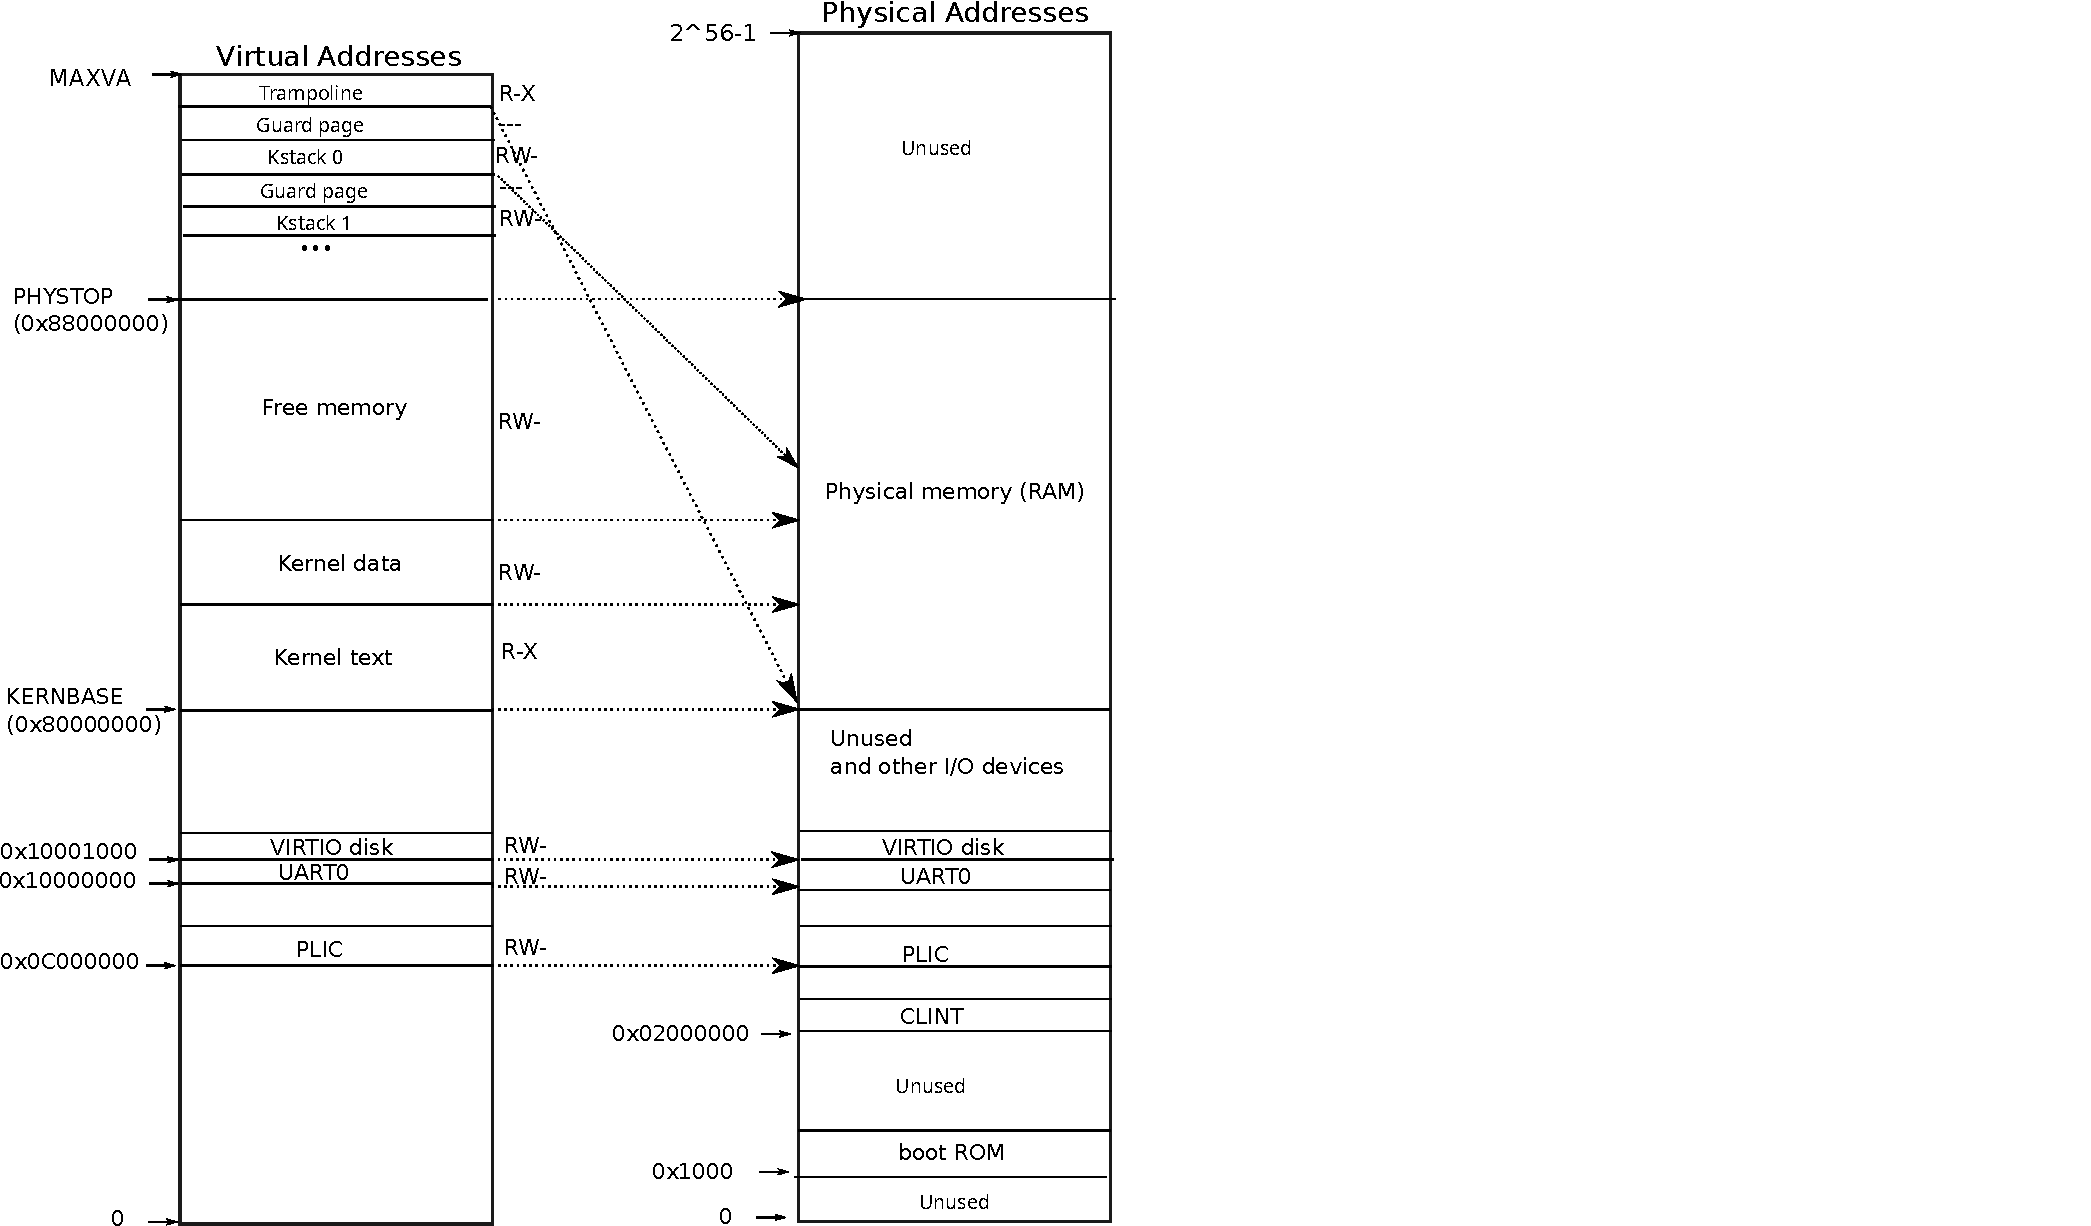
\includegraphics[scale=0.65]{fig/xv6_layout.pdf}
\caption{On the left, xv6's kernel address space.
{\sf \small{RWX}}
refer to PTE read, write, and execute permissions.
On the right, the RISC-V physical address space that
xv6 expects to see.}
\label{fig:xv6_layout}
\end{figure}

%% 
\section{Kernel address space}
%% 
Xv6 maintains one page table per process, describing each
process's user address space, plus a single page table
that describes the kernel's address space.
The kernel configures the layout of its address space to
give itself
access to physical memory and
various hardware resources at predictable virtual addresses.
Figure~\ref{fig:xv6_layout}
shows how this layout maps
kernel virtual addresses to physical addresses.  The file
\fileref{kernel/memlayout.h}
declares the constants for xv6's kernel memory layout.

QEMU simulates a computer that includes RAM (physical memory) starting
at physical address \texttt{0x80000000} and continuing through
at least \texttt{0x88000000}, which xv6 calls \texttt{PHYSTOP}.
The QEMU simulation also
includes I/O devices
such as a disk interface.
QEMU exposes the device interfaces to software as
\indextext{memory-mapped}
control registers that sit below
\texttt{0x80000000}
in the physical address space.
The kernel can interact with the devices by reading/writing
these special physical addresses; such reads and writes communicate
with the device hardware rather than with RAM.
Chapter~\ref{CH:TRAP} explains
how xv6 interacts with devices.

The kernel gets at RAM and memory-mapped device registers
using ``direct mapping;'' that is, mapping the resources at
virtual addresses that are equal to the physical address.
For
example, the kernel itself is located at \lstinline{KERNBASE=0x80000000} in both
the virtual address space and in physical memory.
Direct mapping simplifies kernel code that reads or writes
physical memory. For example, when \lstinline{fork}
allocates user memory for the child process,
the allocator returns the physical address of that memory;
\lstinline{fork} uses that address directly as a virtual
address when it is copying the parent's user memory to the child.

There are a couple of kernel virtual
addresses that aren't direct-mapped:

\begin{itemize}
  
\item The trampoline page. It is mapped at the top of the virtual
  address space; user page tables have this same mapping.
  Chapter~\ref{CH:TRAP} discusses the role of the trampoline
  page, but we see here an interesting use case of page tables; a
  physical page (holding the trampoline code) is mapped twice in the
  virtual address space of the kernel: once at top of the virtual
  address space and once with a direct mapping.

\item The kernel stack pages.  Each process has its own kernel stack,
  which is mapped high so that below it xv6 can leave an unmapped \indextext{guard
    page}.  The guard page's PTE is invalid (i.e.,
  \lstinline{PTE_V} is not set), so that if the kernel overflows
  a kernel stack, it will likely cause an exception and the kernel will panic.
  Without a guard page an overflowing stack would overwrite other kernel memory,
  resulting in incorrect operation. A panic crash is preferable.

\end{itemize}

While the kernel uses its stacks via the high-memory mappings, they
are also accessible to the kernel through a direct-mapped address. An
alternate design might have just the direct mapping, and use the
stacks at the direct-mapped address. In that arrangement, however,
providing guard pages would involve unmapping virtual addresses that
would otherwise refer to physical memory, which would then be hard to
use.

The kernel maps the pages for the trampoline and the kernel text with
the permissions
\lstinline{PTE_R}
and
\lstinline{PTE_X}.
The kernel reads and executes instructions from these pages.
The kernel maps the other pages with the permissions
\lstinline{PTE_R}
and
\lstinline{PTE_W},
so that it can read and write the memory in those pages.
The mappings for the guard pages are invalid.


%% 
\section{Code: creating an address space}
%% 

Most of the xv6 code for manipulating address spaces and
page tables resides in {\tt vm.c}
\lineref{kernel/vm.c:1}.
The central data structure is {\tt pagetable\_t}, which
is really a pointer to a RISC-V root page-table page;
a {\tt pagetable\_t} may be either the kernel
page table, or one of the per-process page tables.
The central functions are {\tt walk},
which finds the PTE for a virtual address,
and {\tt mappages}, which installs PTEs for new mappings.
Functions starting with {\tt kvm} manipulate
the kernel page table; functions starting with {\tt uvm}
manipulate a user page table; other functions are
used for both.
{\tt copyout} and {\tt copyin} copy data to and from
user virtual addresses provided as system call arguments;
they are in {\tt vm.c} because they need to explicitly
translate those addresses in order to find the corresponding
physical memory.

Early in the boot sequence,
\indexcode{main}
calls
\indexcode{kvminit}
\lineref{kernel/vm.c:/^kvminit/}
to create the kernel's page table using
\indexcode{kvmmake}
\lineref{kernel/vm.c:/^kvmmake/}.
This call occurs before xv6 has enabled paging on the RISC-V,
so addresses refer directly to physical memory.
\lstinline{kvmmake}
first allocates a page of physical memory to hold the root page-table page.
Then it calls
\indexcode{kvmmap}
to install the translations that the kernel needs.
The translations include the kernel's
instructions and data, physical memory up to
\indexcode{PHYSTOP},
and memory ranges which are actually devices.
\indexcode{proc_mapstacks}
\lineref{kernel/proc.c:/^proc_mapstacks/}
allocates a kernel stack for each
process. It calls \lstinline{kvmmap} to map each stack at the virtual address generated by
\lstinline{KSTACK}, which leaves room for the invalid stack-guard
pages.

\indexcode{kvmmap} 
\lineref{kernel/vm.c:/^kvmmap/}
calls
\indexcode{mappages}
\lineref{kernel/vm.c:/^mappages/},
which
installs mappings into a page table
for a range of virtual addresses to
a corresponding range of physical addresses.
It does this separately for each virtual address in the range,
at page intervals.
For each virtual address to be mapped,
\lstinline{mappages}
calls
\indexcode{walk}
to find the address of the PTE for that address.
It then initializes the PTE to hold the relevant physical page
number, the desired permissions 
(\lstinline{PTE_W},
\lstinline{PTE_X},
and/or
\lstinline{PTE_R}),
and
\lstinline{PTE_V}
to mark the PTE as valid
\lineref{kernel/vm.c:/perm...PTE_V/}.

\indexcode{walk}
\lineref{kernel/vm.c:/^walk/}
mimics the RISC-V paging hardware as it
looks up the PTE for a virtual address (see
Figure~\ref{fig:riscv_pagetable}).
\lstinline{walk}
descends the page table one level at a time,
using each level's 9 bits of virtual address to
index into the relevant page directory page.
At each level it finds either the PTE of the
next level's page directory page, or the PTE of
final page
\lineref{kernel/vm.c:/pte.=..pagetable/}.
If a PTE in a first or second level page directory
page isn't valid, then the required directory page
hasn't yet been allocated;
if the
\lstinline{alloc}
argument is set,
\lstinline{walk}
allocates a new page-table page and puts its physical address in the PTE.
It returns the address of the PTE in the lowest layer in the tree
\lineref{kernel/vm.c:/return..pagetable/}.

The above code depends on physical memory being direct-mapped into the
kernel virtual address space. For example, as \lstinline{walk} descends levels
of the page table, it pulls the (physical) address of the
next-level-down page table from a PTE \lineref{kernel/vm.c:/pagetable.=..pa.*E2P/},
and then uses that address as a
virtual address to fetch the PTE at the next level down
\lineref{kernel/vm.c:/t..pte.=..paget/}.

\indexcode{main}
calls
\indexcode{kvminithart}
\lineref{kernel/vm.c:/^kvminithart/}
to install the kernel page table.
It writes the physical address of the root page-table page
into the register
\texttt{satp}.
After this the CPU will translate addresses using the kernel
page table.  Since the kernel uses a direct mapping, the now
virtual address of the next instruction will map to the right physical
memory address.

Each RISC-V CPU caches page table entries in a
\indextext{Translation Look-aside Buffer (TLB)}, and when xv6 changes
a page table, it must tell the CPU to invalidate corresponding
cached TLB entries.  If it didn't,
then at some point later the TLB might
use an old cached mapping, pointing to a physical page that in the meantime
has been allocated to another process, and as a result, a process
might be able to scribble on some other process's memory.  The RISC-V
has an instruction \indexcode{sfence.vma} that flushes
the current CPU's TLB.
Xv6 executes {\tt sfence.vma} in {\tt kvminithart}  after reloading the 
\texttt{satp} register, and in the trampoline code that
switches to a user page table before returning to user space
\lineref{kernel/trampoline.S:/sfence.vma/}.

It is also necessary to issue \texttt{sfence.vma} before changing
\texttt{satp}, in order to wait for completion of all outstanding loads and
stores. This wait ensures that preceding updates to the page table have
completed, and ensures that preceding loads and stores use the old
page table, not the new one.

To avoid flushing the complete TLB, RISC-V CPUs may support address
space identifiers (ASIDs)~\cite{riscv:priv}.  The kernel can then
flush just the TLB entries for a particular address space. Xv6
does not use this feature.

\section{Physical memory allocation}

The kernel must allocate and free physical memory at run-time for
page tables,
user memory,
kernel stacks,
and pipe buffers.

Xv6 uses the physical memory between the end of the kernel and
\indexcode{PHYSTOP}
for run-time allocation. It allocates and frees whole 4096-byte pages
at a time. It keeps track of which pages are free by threading a
linked list through the pages themselves. Allocation consists of
removing a page from the linked list; freeing consists of adding the
freed page to the list.
%% 
\section{Code: Physical memory allocator}
%% 

The allocator resides in {\tt kalloc.c} \lineref{kernel/kalloc.c:1}.
The allocator's data structure is a
\textit{free list}
of physical memory pages that are available
for allocation.
Each free page's list element is a
\indexcode{struct run}
\lineref{kernel/kalloc.c:/^struct.run/}.
Where does the allocator get the memory
to hold that data structure?
It store each free page's
\lstinline{run}
structure in the free page itself,
since there's nothing else stored there.
The free list is
protected by a spin lock
\linerefs{kernel/kalloc.c:/^struct.{/,/}/}.
The list and the lock are wrapped in a struct
to make clear that the lock protects the fields
in the struct.
For now, ignore the lock and the calls to
\lstinline{acquire}
and
\lstinline{release};
Chapter~\ref{CH:LOCK} will examine
locking in detail.

The function
\indexcode{main}
calls
\indexcode{kinit}
to initialize the allocator
\lineref{kernel/kalloc.c:/^kinit/}.
\lstinline{kinit}
initializes the free list to hold
every page between the end of the kernel and {\tt PHYSTOP}.
Xv6 ought to determine how much physical
memory is available by parsing configuration information 
provided by the hardware.
Instead xv6 assumes that the machine has
128 megabytes of RAM.
\lstinline{kinit}
calls
\indexcode{freerange}
to add memory to the free list via per-page calls to
\indexcode{kfree}.
A PTE can only refer to a physical address that is aligned
on a 4096-byte boundary (is a multiple of 4096), so
\lstinline{freerange}
uses
\indexcode{PGROUNDUP}
to ensure that it frees only aligned physical addresses.
The allocator starts with no memory;
these calls to
\lstinline{kfree}
give it some to manage.

The allocator sometimes treats addresses as integers
in order to perform arithmetic on them (e.g.,
traversing all pages in
\lstinline{freerange}),
and sometimes uses addresses as pointers to read and
write memory (e.g., manipulating the
\lstinline{run}
structure stored in each page);
this dual use of addresses is the main reason that the
allocator code is full of C type casts.
\index{type cast}

The function
\lstinline{kfree}
\lineref{kernel/kalloc.c:/^kfree/}
begins by setting every byte in the
memory being freed to the value 1.
This will cause code that uses memory after freeing it
(uses ``dangling references'')
to read garbage instead of the old valid contents;
hopefully that will cause such code to break faster.
Then
\lstinline{kfree}
prepends the page to the free list:
it casts
\lstinline{pa}
to a pointer to
\lstinline{struct}
\lstinline{run},
records the old start of the free list in
\lstinline{r->next},
and sets the free list equal to
\lstinline{r}.
\indexcode{kalloc}
removes and returns the first element in the free list.

\section{Process address space}

Each process has its own page table, and when xv6 switches between
processes, it also changes page tables.
Figure~\ref{fig:processlayout} shows a process's address space in more
detail than Figure~\ref{fig:as}.  A process's user memory starts at
virtual address zero and can grow up to \texttt{MAXVA}
\lineref{kernel/riscv.h:/MAXVA/}, allowing a process to address in
principle 256 Gigabytes of memory.

A process's address space consists of pages that contain the text of
the program (which xv6 maps with the permissions \lstinline{PTE_R},
\lstinline{PTE_X}, and \lstinline{PTE_U}), pages that contain the
pre-initialized data of the program, a page for the stack, and pages
for the heap.  Xv6 maps the data, stack, and heap with the permissions
\lstinline{PTE_R}, \lstinline{PTE_W}, and \lstinline{PTE_U}.

Using permissions within a user address space is a common technique to
harden a user process.  If the text were mapped with
\lstinline{PTE_W}, then a process could accidentally modify its own
program; for example, a programming error may cause the program to
write to a null pointer, modifying instructions at address 0, and then
continue running, perhaps creating more havoc.  To detect such errors
immediately, xv6 maps the text without \lstinline{PTE_W}; if a program
accidentally attempts to store to address 0, the hardware will refuse
to execute the store and raises a page fault (see
Section~\ref{sec:pagefaults}).  The kernel then kills the process and
prints out an informative message so that the developer can track down
the problem.

Similarly, by mapping data without \lstinline{PTE_X}, a user program
cannot accidentally jump to an address in the program's data and start
executing at that address.

In the real world, hardening a process by setting permissions
carefully also aids in defending against security attacks.  An
adversary may feed carefully-constructed input to a program (e.g., a
Web server) that triggers a bug in the program in the hope of turning
that bug into an exploit~\cite{aleph:smashing}.  Setting permissions
carefully and other techniques, such as randomizing of the layout of the
user address space, make such attacks harder.

The stack is a single page, and is shown with the initial contents as
created by exec.  Strings containing the command-line arguments, as
well as an array of pointers to them, are at the very top of the
stack.  Just under that are values that allow a program to start at
\lstinline{main} as if the function \lstinline{main(argc},
\lstinline{argv)} had just been called.

To detect a user stack overflowing the allocated stack memory, xv6
places an inaccessible guard page right below the stack by clearing
the \lstinline{PTE_U} flag. If the user stack overflows and the
process tries to use an address below the stack, the hardware will
generate a page-fault exception because the guard page is inaccessible
to a program running in user mode. A real-world operating system might
instead automatically allocate more memory for the user stack when it
overflows.

When a process asks xv6 for more user memory, xv6 grows the process's
heap. Xv6 first uses {\tt kalloc} to allocate physical pages.
It then adds PTEs to the process's page table that point
to the new physical pages.
Xv6 sets the
\lstinline{PTE_W},
\lstinline{PTE_R},
\lstinline{PTE_U},
and
\lstinline{PTE_V}
flags in these PTEs.
Most processes do not use the entire user address space;
xv6 leaves
\lstinline{PTE_V}
clear in unused PTEs.

We see here a few nice examples of use of page tables.  First,
different processes' page tables translate user addresses to different
pages of physical memory, so that each process has private user
memory.  Second, each process sees its memory as having contiguous
virtual addresses starting at zero, while the process's physical
memory can be non-contiguous.  Third, the kernel maps a page with
trampoline code at the top of the user address space (without
\lstinline{PTE_U}), thus a single page of physical memory shows up in
all address spaces, but can be used only by the kernel.

\begin{figure}[t]
\center
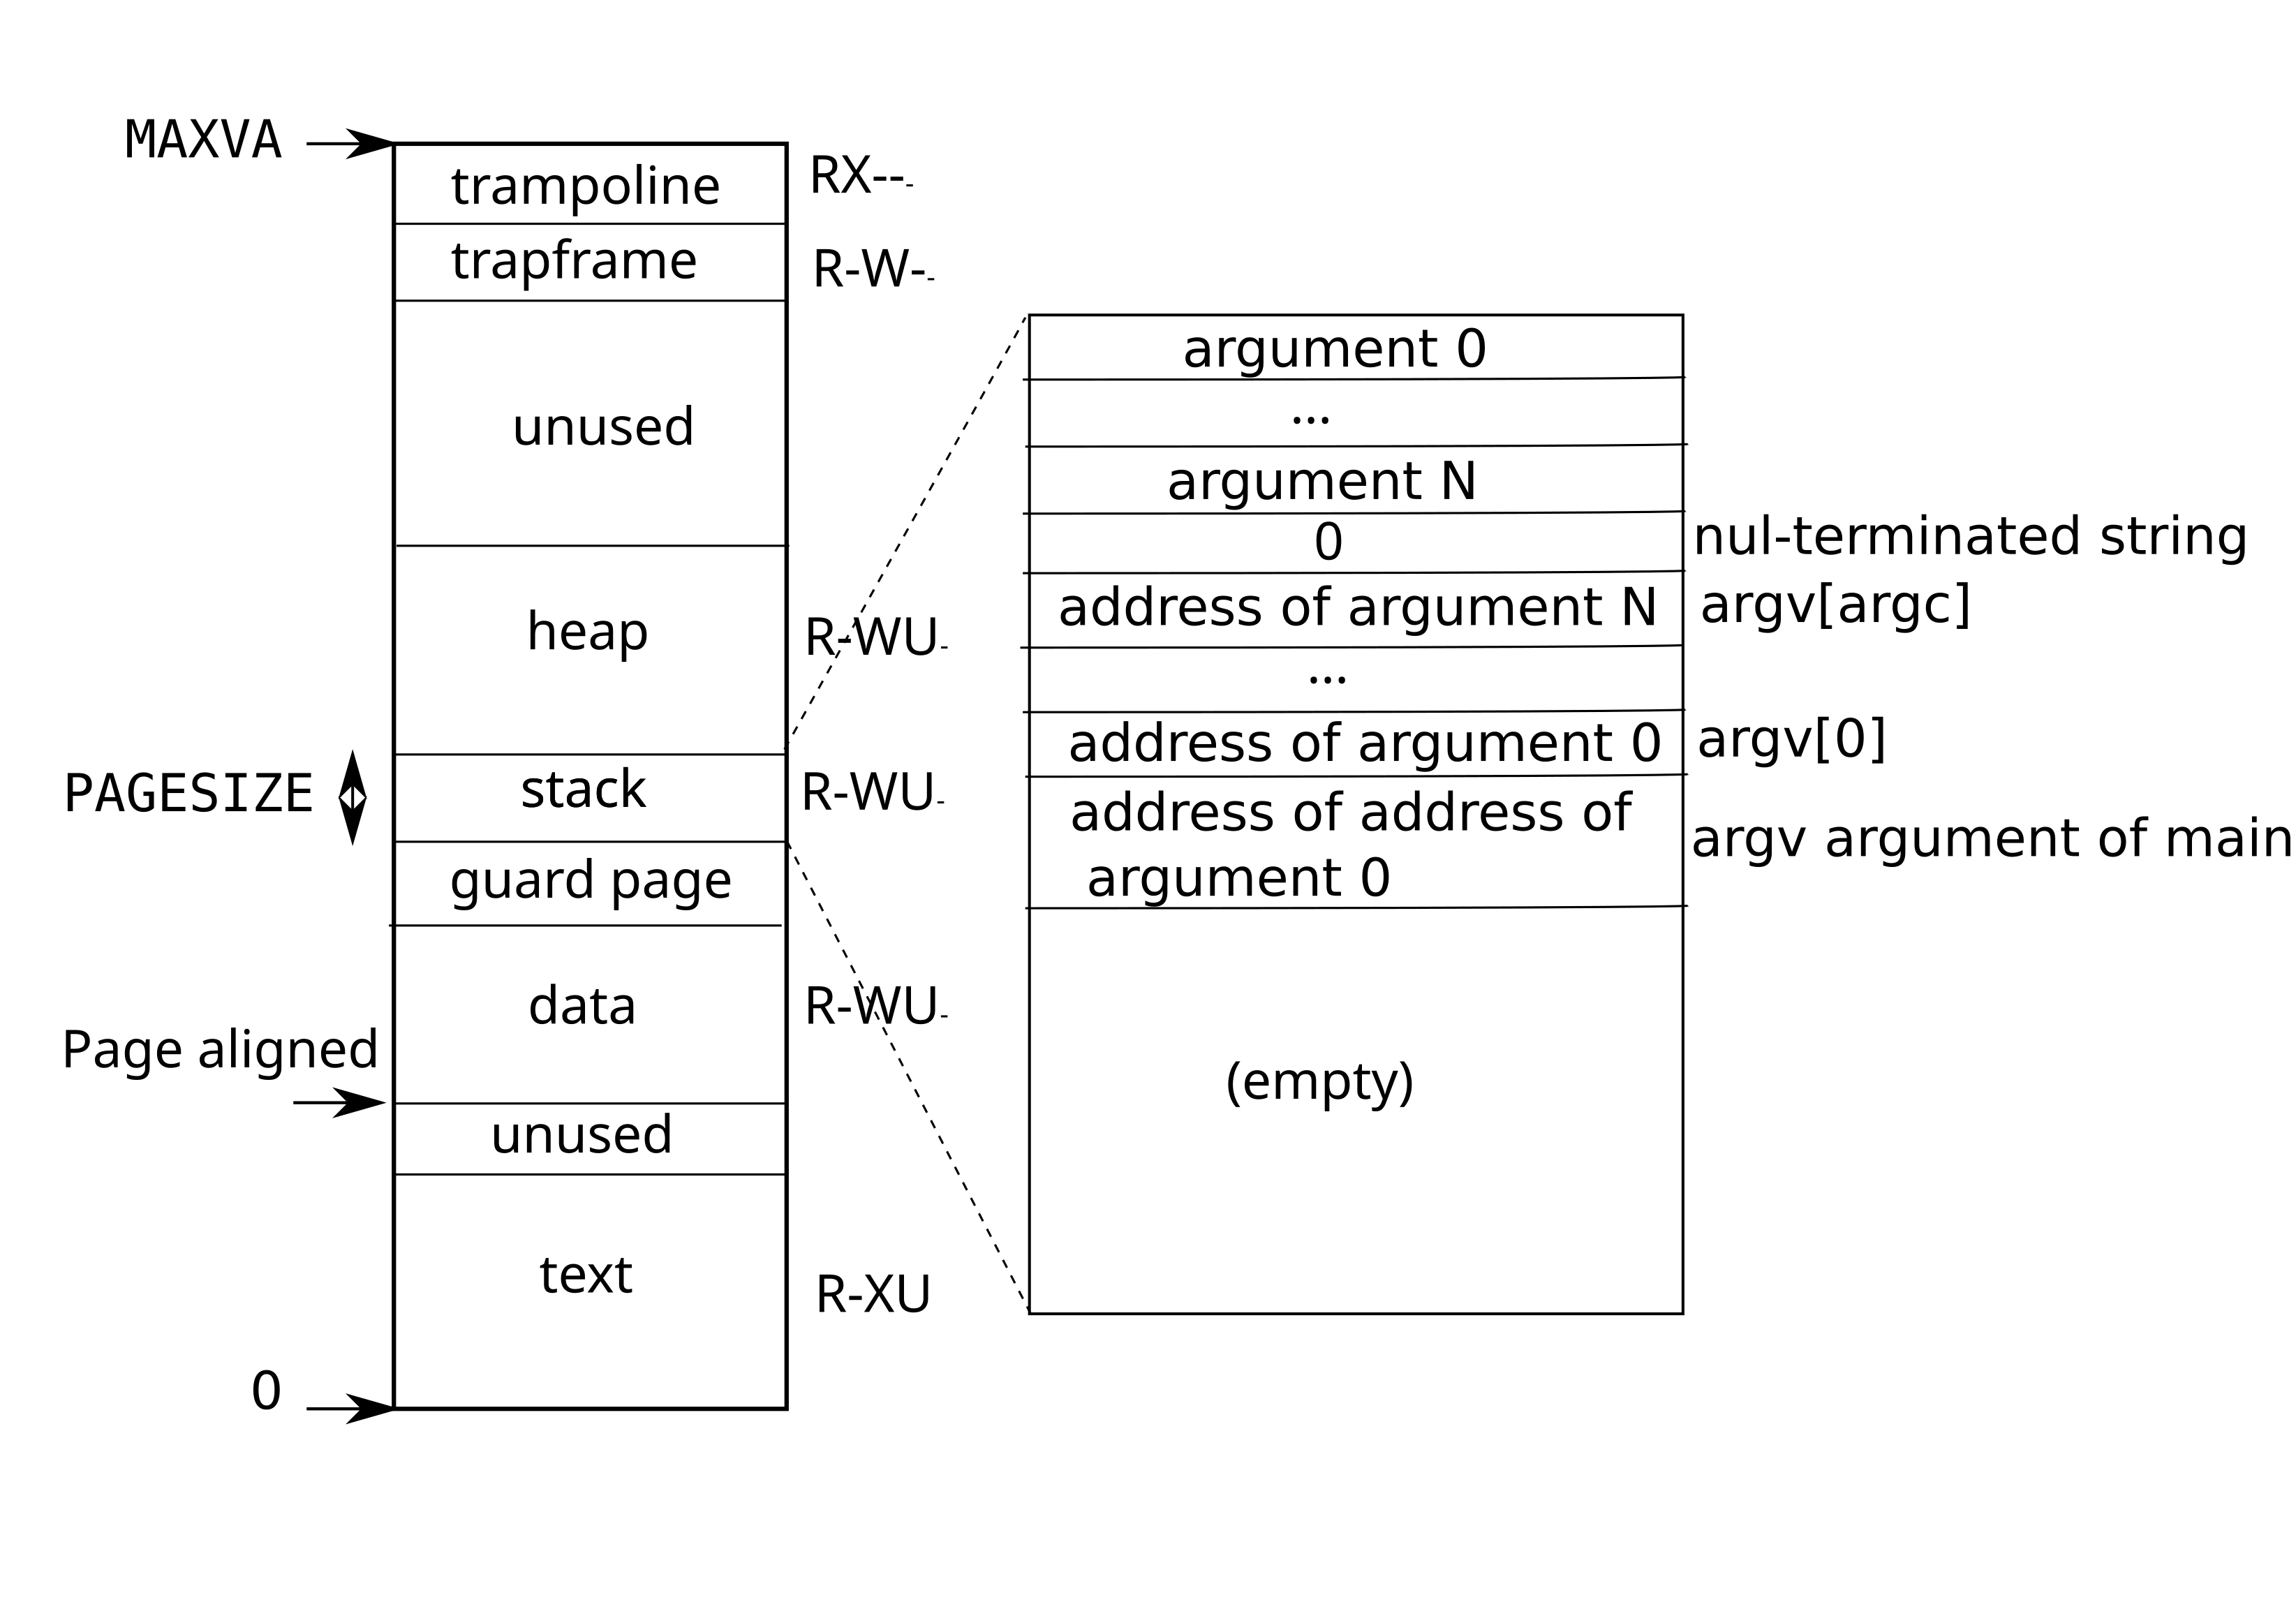
\includegraphics[scale=0.5]{fig/processlayout.png}
\caption{A process's user address space, with its initial stack.}
\label{fig:processlayout}
\end{figure}

\section{Code: sbrk}

\lstinline{sbrk}
is the system call for a process to shrink or grow its memory. The system
call is implemented by the function
\lstinline{growproc}
\lineref{kernel/proc.c:/^growproc/}.
\lstinline{growproc} calls \lstinline{uvmalloc} or
\lstinline{uvmdealloc}, depending on whether \lstinline{n} is positive
or negative.
\lstinline{uvmalloc}
\lineref{kernel/vm.c:/^uvmalloc/}
allocates physical memory with {\tt kalloc}, zeros the allocated memory,
and adds PTEs to the user page table with {\tt mappages}.
\lstinline{uvmdealloc} calls
{\tt uvmunmap}
\lineref{kernel/vm.c:/^uvmunmap/},
which uses {\tt walk} to find PTEs and
{\tt kfree} to free the physical memory they refer to.

Xv6 uses a process's page table not just to tell the hardware how to
map user virtual addresses, but also as the only record of which
physical memory pages are allocated to that process. That is the
reason why freeing user memory (in {\tt uvmunmap}) requires
examination of the user page table.

%% 
\section{Code: exec}
%% 
\lstinline{exec} is a system call that replaces a process's
user address space with data read from a file, called a binary
or executable file.
A binary is typically the output of the compiler and linker,
and holds machine instructions and program data.
\lstinline{exec} \lineref{kernel/exec.c:/^exec/} opens the
named binary \lstinline{path} using \indexcode{namei}
\lineref{kernel/exec.c:/namei/}, which is explained in
Chapter~\ref{CH:FS}.  Then, it reads the ELF header. Xv6 binaries
are formatted in the widely-used \indextext{ELF format}, defined in
\fileref{kernel/elf.h}.  An ELF binary consists of an ELF header,
\indexcode{struct elfhdr} \lineref{kernel/elf.h:/^struct.elfhdr/},
followed by a sequence of program section headers,
\lstinline{struct proghdr} \lineref{kernel/elf.h:/^struct.proghdr/}.  Each
\lstinline{progvhdr} describes a section of the application that must
be loaded into memory; xv6 programs have two program section
headers: one for instructions and one for data.

The first step is a quick check that the file probably contains an
ELF binary.
An ELF binary starts with the four-byte ``magic number''
\lstinline{0x7F},
\lstinline{`E'},
\lstinline{`L'},
\lstinline{`F'},
or
\indexcode{ELF_MAGIC}
\lineref{kernel/elf.h:/ELF_MAGIC/}.
If the ELF header has the right magic number,
\lstinline{exec}
assumes that the binary is well-formed.

\lstinline{exec}
allocates a new page table with no user mappings with
\indexcode{proc_pagetable}
\lineref{kernel/exec.c:/proc_pagetable/},
allocates memory for each ELF segment with
\indexcode{uvmalloc}
\lineref{kernel/exec.c:/uvmalloc/},
and loads each segment into memory with
\indexcode{loadseg}
\lineref{kernel/exec.c:/loadseg/}.
\lstinline{loadseg}
uses
\indexcode{walkaddr}
to find the physical address of the allocated memory at which to write
each page of the ELF segment, and
\indexcode{readi}
to read from the file.

The program section header for
\indexcode{/init},
the first user program created with
\lstinline{exec},
looks like this:
\begin{footnotesize}
\begin{verbatim}
# objdump -p user/_init

user/_init:     file format elf64-little

Program Header:
0x70000003 off    0x0000000000006bb0 vaddr 0x0000000000000000
                                       paddr 0x0000000000000000 align 2**0
         filesz 0x000000000000004a memsz 0x0000000000000000 flags r--
    LOAD off    0x0000000000001000 vaddr 0x0000000000000000
                                       paddr 0x0000000000000000 align 2**12
         filesz 0x0000000000001000 memsz 0x0000000000001000 flags r-x
    LOAD off    0x0000000000002000 vaddr 0x0000000000001000
                                       paddr 0x0000000000001000 align 2**12
         filesz 0x0000000000000010 memsz 0x0000000000000030 flags rw-
   STACK off    0x0000000000000000 vaddr 0x0000000000000000
                                       paddr 0x0000000000000000 align 2**4
         filesz 0x0000000000000000 memsz 0x0000000000000000 flags rw-
\end{verbatim}
\end{footnotesize}

We see that the text segment should be loaded at virtual address 0x0
in memory (without write permissions) from content at offset
0x1000 in the file. We also see that the data should be loaded at
address 0x1000, which is at a page boundary, and without executable
permissions.

A program section header's
\lstinline{filesz}
may be less than the
\lstinline{memsz},
indicating that the gap between them should be filled
with zeroes (for C global variables) rather than read from the file.
For
\lstinline{/init}, the data
\lstinline{filesz}
is 0x10 bytes and
\lstinline{memsz}
is 0x30 bytes,
and thus
\indexcode{uvmalloc}
allocates enough physical memory to hold 0x30 bytes, but reads only 0x10 bytes
from the file
\lstinline{/init}.

Now
\indexcode{exec}
allocates and initializes the user stack.
It allocates just one stack page.
\lstinline{exec}
copies the argument strings to the top of the stack
one at a time, recording the pointers to them in
\indexcode{ustack}.
It places a null pointer at the end of what will be the
\indexcode{argv}
list passed to
\lstinline{main}.
The values for \indexcode{argc} and \lstinline{argv} are passed to \lstinline{main}
through the system-call return path:  \lstinline{argc} is passed via the
system call return value, which goes in {\tt a0}, and \lstinline{argv} is passed through
the {\tt a1} entry of the process's trapframe.

\lstinline{exec}
places an inaccessible page just below the stack page,
so that programs that try to use more than one page will fault.
This inaccessible page also allows
\lstinline{exec}
to deal with arguments that are too large;
in that situation,
the
\indexcode{copyout}
\lineref{kernel/vm.c:/^copyout/}
function that
\lstinline{exec}
uses to copy arguments to the stack will notice that
the destination page is not accessible, and will
return -1.

During the preparation of the new memory image,
if
\lstinline{exec}
detects an error like an invalid program segment,
it jumps to the label
\lstinline{bad},
frees the new image,
and returns -1.
\lstinline{exec}
must wait to free the old image until it
is sure that the system call will succeed:
if the old image is gone,
the system call cannot return -1 to it.
The only error cases in
\lstinline{exec}
happen during the creation of the image.
Once the image is complete,
\lstinline{exec}
can commit to the new page table
\lineref{kernel/exec.c:/pagetable.=.pagetable/}
and free the old one
\lineref{kernel/exec.c:/proc_freepagetable/}.

\lstinline{exec}
loads bytes from the ELF file into memory at addresses specified by the ELF file.
Users or processes can place whatever addresses they want into an ELF file.
Thus
\lstinline{exec}
is risky, because the addresses in the ELF file may refer to the kernel, accidentally
or on purpose. The consequences for an unwary kernel could range from
a crash to a malicious subversion of the kernel's isolation mechanisms
(i.e., a security exploit).
Xv6 performs a number of checks to avoid these risks.
For example
\lstinline{if(ph.vaddr + ph.memsz < ph.vaddr)}
checks for whether the sum overflows a 64-bit integer.
The danger is that a user could construct an ELF binary with a
\lstinline{ph.vaddr}
that points to a user-chosen address,
and
\lstinline{ph.memsz}
large enough that the sum overflows to 0x1000, which will look like a
valid value. In an older version of xv6 in which the user address
space also contained the kernel (but not readable/writable in user
mode), the user could choose an address that corresponded to kernel
memory and would thus copy data from the ELF binary into the kernel.
In the RISC-V version of xv6 this cannot happen, because the kernel has
its own separate page table;
\lstinline{loadseg}
loads into the process's page table, not in the kernel's page table.

It is easy for a kernel developer to omit a crucial check, and
real-world kernels have a long history of missing checks whose absence
can be exploited by user programs to obtain kernel privileges.  It is likely that xv6 doesn't do a complete job of validating
user-level data supplied to the kernel, which a malicious user program might be able to exploit to circumvent xv6's isolation.
%% 
\section{Real world}
%% 

Like most operating systems, xv6 uses the paging hardware for memory
protection and mapping.  Most operating systems make far more
sophisticated use of paging than xv6 by combining paging and
page-fault exceptions, which we will discuss in
Chapter~\ref{CH:TRAP}.

Xv6 is simplified by the kernel's use of a direct map between virtual
and physical addresses, and by its assumption that there is physical
RAM at address 0x80000000, where the kernel expects to be loaded. This
works with QEMU, but on real hardware it turns out to be a bad idea;
real hardware places RAM and devices at unpredictable physical
addresses, so that (for example) there might be no RAM at 0x80000000,
where xv6 expect to be able to store the kernel. More serious kernel
designs exploit the page table to turn arbitrary hardware physical
memory layouts into predictable kernel virtual address layouts.

RISC-V supports protection at the level of physical addresses,
but xv6 doesn't use that feature.

On machines with lots of memory
it might make sense to use
RISC-V's support for ``super pages.''
Small pages make sense
when physical memory is small, to allow allocation and page-out to disk
with fine granularity.
For example, if a program
uses only 8 kilobytes of memory, giving it a whole 4-megabyte super-page
of physical memory is wasteful.
Larger pages make sense on machines with lots of RAM,
and may reduce overhead for page-table manipulation.

The xv6 kernel's lack of a {\tt malloc}-like allocator that can
provide memory for small objects prevents the kernel from using
sophisticated data structures that would require dynamic allocation.
A more elaborate kernel
would likely allocate many different sizes of small blocks,
rather than (as in xv6) just 4096-byte blocks;
a real kernel
allocator would need to handle small allocations as well as large
ones.

Memory allocation is a perennial hot topic, the basic problems being
efficient use of limited memory and
preparing for unknown future requests~\cite{knuth}.  Today people care more about speed than
space efficiency.
%% 
\section{Exercises}
%% 

\begin{enumerate}
  
\item Parse RISC-V's device tree to find the amount of physical memory
the computer has.

\item Write a user program that grows its address space by one byte by calling
\lstinline{sbrk(1)}.
Run the  program and investigate the page table for the program before the call
to
\lstinline{sbrk}
and after the call to
\lstinline{sbrk}.
How much space has the kernel allocated?  What does the
PTE
for the new memory contain?

\item Modify xv6 to use super pages for the kernel.

\item Unix implementations of
\lstinline{exec}
traditionally include special handling for shell scripts.
If the file to execute begins with the text
\lstinline{#!},
then the first line is taken to be a program
to run to interpret the file.
For example, if
\lstinline{exec}
is called to run
\lstinline{myprog}
\lstinline{arg1}
and
\lstinline{myprog} 's
first line is
\lstinline{#!/interp},
then
\lstinline{exec}
runs
\lstinline{/interp}
with command line
\lstinline{/interp}
\lstinline{myprog}
\lstinline{arg1}.
Implement support for this convention in xv6.

\item Implement address space layout randomization for the kernel.

\end{enumerate}

%    Sidebar about panic:
% 	panic is the kernel's last resort: the impossible has happened and the
% 	kernel does not know how to proceed.  In xv6, panic does ...
\chapter{Traps and system calls}
\label{CH:TRAP}

There are three kinds of event which cause the CPU to set
aside ordinary execution of instructions and force a
transfer of control to special code that handles the event. One
situation is a system call, when a user program 
executes the {\tt ecall} instruction to ask the kernel to do 
something for it. Another situation is an \indextext{exception}:
an instruction (user or kernel) does something illegal, such as divide
by zero or use an invalid virtual address. The third situation is a
device \indextext{interrupt}, when a device signals that it needs
attention, for example when the disk hardware finishes a read or write
request.

This book uses \indextext{trap} as a generic term for these
situations. Typically whatever code was executing at the time of the
trap will later need to resume, and shouldn't need to be aware that
anything special happened. That is, we often want traps to be
transparent; this is particularly important for device interrupts, which the
interrupted code typically doesn't expect. The usual sequence is that
a trap forces a transfer of control into the kernel; the kernel saves
registers and other state so that execution can be resumed; the kernel
executes appropriate handler code (e.g., a system call implementation
or device driver); the kernel restores the saved state and returns
from the trap; and the original code resumes where it left off.

Xv6 handles all traps in the kernel; traps are not delivered to user
code. Handling traps in the kernel is natural for system calls. It
makes sense for interrupts since isolation demands that only the
kernel be allowed to use devices,
and because the kernel is a convenient mechanism with which to
share devices among multiple processes.
It also makes sense for exceptions
since xv6 responds to all exceptions from user space by killing the
offending program.

Xv6 trap handling proceeds in four stages: hardware actions taken by
the RISC-V CPU, some assembly instructions that prepare the way for
kernel C code, a C function that decides what to do with the trap,
and the system call or device-driver service routine. While
commonality among the three trap types suggests that a kernel could
handle all traps with a single code path, it turns out to be
convenient to have separate code for
three distinct cases: traps from user space, traps from kernel space,
and timer interrupts. Kernel code (assembler or C) that
processes a trap is often called a \indextext{handler};
the first handler instructions are usually written in assembler
(rather than C) and are sometimes called a \indextext{vector}.


\section{RISC-V trap machinery}

Each RISC-V CPU has a set of control registers that the kernel writes to
tell the CPU how to handle traps, and that the kernel can read
to find out about a trap that has occurred. The RISC-V documents
contain the full story~\cite{riscv:priv}. {\tt riscv.h}
\lineref{kernel/riscv.h:1} contains definitions that xv6 uses. Here's
an outline of the most important registers:

\begin{itemize}

\item \indexcode{stvec}: The kernel writes the address of its trap handler
  here; the RISC-V jumps to the address in {\tt stvec} to handle a trap.

\item \indexcode{sepc}: When a trap occurs, RISC-V saves the program counter
  here (since the {\tt pc} is then overwritten with the
  value in {\tt stvec}). The
  {\tt sret} (return from trap) instruction copies {\tt sepc} to the
  {\tt pc}. The kernel can write {\tt sepc} to control where {\tt
    sret} goes.

\item \indexcode{scause}: RISC-V puts a number here that describes
the reason for the trap.

\item \indexcode{sscratch}: The trap handler code uses {\tt sscratch}
  to help it avoid overwriting user registers before saving them.

\item \indexcode{sstatus}: The SIE bit in {\tt sstatus}
  controls whether device interrupts
  are enabled. If the kernel clears SIE, the RISC-V will defer
  device interrupts until the kernel sets SIE. The SPP bit
  indicates whether a trap came from user mode or supervisor
  mode, and controls to what mode {\tt sret} returns.

\end{itemize}

The above registers relate to traps handled in supervisor mode, and they
cannot be read or written in user mode. There is a similar set of
control registers for traps handled in machine mode; xv6 uses
them only for the special case of timer interrupts.

Each CPU on a multi-core chip has its own set of these registers,
and more than one CPU may be handling a trap at any given time.

When it needs to force a trap, the RISC-V hardware does the
following for all trap types (other than timer interrupts):

\begin{enumerate}

\item If the trap is a device interrupt, and the {\tt sstatus} SIE bit
  is clear, don't do any of the following.

\item Disable interrupts by clearing the SIE bit in {\tt sstatus}.

\item Copy the {\tt pc} to {\tt sepc}.

\item Save the current mode (user or supervisor) in the SPP bit in {\tt sstatus}.

\item Set {\tt scause} to reflect the trap's cause.

\item Set the mode to supervisor.

\item Copy {\tt stvec} to the {\tt pc}.

\item Start executing at the new {\tt pc}.

\end{enumerate}

Note that the CPU doesn't switch to the kernel page table, doesn't
switch to a stack in the kernel, and doesn't save any registers other
than the {\tt pc}. Kernel software must perform these tasks.
One reason that the CPU does minimal work during a trap is to provide
flexibility to software; for example, some operating systems 
omit a page table switch in some situations to increase
trap performance.

It's worth thinking about whether any of the steps listed above could
be omitted, perhaps in search of faster traps. Though there are
situations in which a simpler sequence can work, many of the steps
would be dangerous to omit in general. For example, suppose that the
CPU didn't switch program counters. Then a trap from user space could
switch to supervisor mode while still running user instructions. Those
user instructions could break user/kernel isolation, for example
by modifying the {\tt satp} register to point to a page table that
allowed accessing all of physical memory. It is thus important that
the CPU switch to a kernel-specified instruction address, namely {\tt
  stvec}.

\section{Traps from user space}

Xv6 handles traps differently depending on whether
the trap occurs while
executing in the kernel or in user code. Here is the
story for traps from user code; Section~\ref{s:ktraps}
describes traps from kernel code.

A trap may occur while executing in user space if the
user program makes a
system call ({\tt ecall} instruction), or does something
illegal, or if a device interrupts.
The high-level path of a trap from user space is
{\tt uservec}
\lineref{kernel/trampoline.S:/^uservec/},
then {\tt usertrap}
\lineref{kernel/trap.c:/^usertrap/};
and when returning,
{\tt usertrapret}
\lineref{kernel/trap.c:/^usertrapret/}
and then
{\tt userret}
\lineref{kernel/trampoline.S:/^userret/}.

% talk about why RISC-V doesn't switch page tables

A major constraint on the design of xv6's trap handling is the fact
that the RISC-V hardware does not switch page tables when it forces a
trap. This means that the trap handler
address in {\tt stvec} must have a valid
mapping in the user page table, since that's the page table in force
when the trap handling code starts executing. Furthermore, xv6's trap
handling code needs to switch to the kernel page table; in order to be
able to continue executing after that switch, the kernel page table
must also have a mapping for the handler pointed to by {\tt stvec}.

Xv6 satisfies these requirements using a \indextext{trampoline} page.
The trampoline page contains {\tt uservec}, the xv6 trap handling code
that {\tt stvec} points to. The trampoline page is mapped in
every process's page table at address
\indexcode{TRAMPOLINE},
which is at the top of the virtual address space so that it will
be above memory that programs use for themselves.
The trampoline page is also mapped at address {\tt TRAMPOLINE}
in the kernel page table. See Figure~\ref{fig:as} and
Figure~\ref{fig:xv6_layout}. Because the trampoline page is mapped in
the user page table, traps can start
executing there in supervisor mode. Because the trampoline page is
mapped at the same address in the kernel address space, the trap handler
can continue to execute after it switches to the kernel page
table.

The code for the {\tt uservec} trap handler is in {\tt trampoline.S}
\lineref{kernel/trampoline.S:/^uservec/}.
When {\tt uservec} starts, all 32 registers contain values owned by
the interrupted user code. These 32 values need to be saved somewhere
in memory, so that later on
the kernel can restore them before returning to user space.
Storing to memory requires use of a register
to hold the address,
but at this point there are no general-purpose registers available!
Luckily RISC-V provides a helping hand in the
form of the {\tt sscratch} register. The {\tt csrw} instruction at
the start of {\tt uservec} saves {\tt a0} in {\tt
  sscratch}. Now 
{\tt uservec} has
one register ({\tt a0}) to play with.

{\tt uservec}'s next task is to save the 32 user registers.
The kernel allocates, for each process, a page of memory for a
{\tt trapframe} structure that (among other things) has space to
save the 32 user registers
\lineref{kernel/proc.h:/^struct.trapframe/}. Because {\tt satp} still
refers to the user page table, {\tt uservec} needs the trapframe to be
mapped in the user address space. Xv6 maps each process's trapframe
at virtual address {\tt TRAPFRAME} in that process's user page table;
{\tt TRAPFRAME} is
just below {\tt TRAMPOLINE}. The process's {\tt p->trapframe} also
points to the
trapframe, though at its physical address so the kernel can use it
through the kernel page table.

Thus {\tt uservec} loads address {\tt TRAPFRAME} into {\tt a0}
and saves all the user registers there,
including the user's {\tt a0}, read back from {\tt sscratch}.

The {\tt trapframe} contains the address of the current process's
kernel stack, the current CPU's hartid, the address of the {\tt usertrap}
function,
and the address of the kernel page table. {\tt uservec}
retrieves these values, switches {\tt satp} to the kernel page table,
and jumps to {\tt usertrap}.

The job of {\tt usertrap} is to determine
the cause of the trap, process it, and return
\lineref{kernel/trap.c:/^usertrap/}.
It first changes {\tt stvec} so
that a trap while in the kernel will be handled by
{\tt kernelvec} rather than {\tt uservec}.
It saves the {\tt sepc} register (the saved user program counter),
because 
{\tt usertrap} might call \lstinline{yield} to switch
to another process's kernel thread, and that process might return
to user space, in the process of which it will modify \lstinline{sepc}.
If the trap is a system call, {\tt usertrap} calls {\tt syscall} to
handle it;
if a device interrupt, {\tt devintr};
otherwise it's an exception, and the kernel kills the
faulting process.
The system call path adds four to the saved user program counter
because RISC-V, in the case of a system call,
leaves the program pointer pointing to the {\tt ecall} instruction
but user code needs to resume executing at the subsequent instruction.
On the way out, {\tt usertrap} checks if the process has been
killed or should yield the CPU (if this trap is a timer interrupt).

The first step in returning to user space is the call to {\tt usertrapret}
\lineref{kernel/trap.c:/^usertrapret/}.
This function sets up the RISC-V control registers to prepare for a
future trap from user space: setting {\tt stvec}
to {\tt uservec} and preparing the trapframe fields that
{\tt uservec} relies on.
{\tt usertrapret} sets {\tt sepc} to the previously
saved user program counter.
At the end, {\tt usertrapret}
calls {\tt userret} on the trampoline page that is mapped in
both user and kernel page tables; the reason is that assembly
code in {\tt userret} will switch page tables.

{\tt usertrapret}'s call to {\tt userret} passes 
a pointer to the process's user page table in {\tt a0}
\lineref{kernel/trampoline.S:/^userret/}.
{\tt userret} switches {\tt satp} to the process's user page table.
Recall that the user page table maps both the trampoline page
and {\tt TRAPFRAME}, but nothing else from the kernel.
The trampoline page mapping at the same
virtual address in user and kernel page tables allows
{\tt userret} to keep executing after changing {\tt satp}.
From this point on, the only data {\tt userret} can use is
the register contents and the content of the trapframe.
{\tt userret} loads the {\tt TRAPFRAME} address into {\tt a0},
restores saved user registers from the trapframe via {\tt a0},
restores the saved user {\tt a0},
and executes {\tt sret} to return to user space.

\section{Code: Calling system calls}

Chapter~\ref{CH:FIRST} ended with 
\indexcode{initcode.S}
invoking the {\tt exec} system call
\lineref{user/initcode.S:/SYS_exec/}.
Let's look at how the user call
makes its way to the {\tt exec} system call's
implementation in the kernel.

{\tt initcode.S}
places the arguments for
\indexcode{exec}
in registers {\tt a0} and {\tt a1}, and puts the
system call number in
\texttt{a7}.
System call numbers match the entries in the {\tt syscalls} array,
a table of function pointers
\lineref{kernel/syscall.c:/syscalls/}.
The \lstinline{ecall} instruction traps into the kernel
and causes
{\tt uservec},
{\tt usertrap}, and then {\tt syscall} to execute, as we saw above.

\indexcode{syscall}
\lineref{kernel/syscall.c:/^syscall/} 
retrieves the system call number from the saved
\texttt{a7} in the trapframe
and uses it to index into {\tt syscalls}.
For the first system call, 
\texttt{a7}
contains 
\indexcode{SYS_exec}
\lineref{kernel/syscall.h:/SYS_exec/},
resulting in a call to the system call implementation function
\lstinline{sys_exec}.

When \lstinline{sys_exec} returns,
\lstinline{syscall}
records its return value in
\lstinline{p->trapframe->a0}.
This will cause the original user-space call to 
{\tt exec()} to return that value, since the C
calling convention on RISC-V places return values in {\tt a0}.
System calls conventionally return negative numbers to indicate
errors, and zero or positive numbers for success.
If the system call number is invalid,
\lstinline{syscall}
prints an error and returns $-1$.

\section{Code: System call arguments}

System call implementations in the kernel need to find the arguments
passed by user code. Because user code calls system call wrapper
functions, the arguments are initially where the RISC-V C calling
convention places them: in registers.
The kernel trap code saves user registers to the current
process's trap frame, where kernel code can find them.
The kernel functions
\lstinline{argint},
\lstinline{argaddr},
and
\lstinline{argfd}
retrieve the 
\textit{n} 'th 
system call argument
from the trap frame
as an integer, pointer, or a file descriptor.
They all call {\tt argraw} to retrieve the appropriate saved
user register
\lineref{kernel/syscall.c:/^argraw/}.

Some system calls pass pointers as arguments, and the kernel must use
those pointers to read or write user memory. The {\tt exec} system
call, for example, passes the kernel an array of pointers
referring to string arguments in user space.
These pointers pose
two challenges. First, the user program may be buggy or malicious, and
may pass the kernel an invalid pointer or a pointer intended to trick
the kernel into accessing kernel memory instead of user memory.
Second, the xv6 kernel page table mappings are not the same as the
user page table mappings, so the kernel cannot use ordinary
instructions to load or store from user-supplied addresses.

The kernel implements functions that safely transfer data to and
from user-supplied addresses.
{\tt fetchstr} is an example \lineref{kernel/syscall.c:/^fetchstr/}.
File system calls such as
{\tt exec} use {\tt fetchstr} to retrieve string file-name arguments from user
space.
\lstinline{fetchstr} calls \lstinline{copyinstr}
to do the hard work.

\indexcode{copyinstr}
\lineref{kernel/vm.c:/^copyinstr/} copies up to \lstinline{max} bytes to
\lstinline{dst} from virtual address \lstinline{srcva} in the user page
table \lstinline{pagetable}.
Since \lstinline{pagetable} is {\it not} the current page
table,
\lstinline{copyinstr} uses {\tt walkaddr}
(which calls {\tt walk}) to look up
\lstinline{srcva} in
\lstinline{pagetable}, yielding
physical address \lstinline{pa0}.
The kernel's page table maps all of physical RAM 
at virtual addresses that are equal to the RAM's physical address.
This allows
{\tt copyinstr} to directly copy string bytes from {\tt pa0} to {\tt dst}.
{\tt walkaddr} 
\lineref{kernel/vm.c:/^walkaddr/}
checks that the user-supplied virtual address is part of
the process's user address space, so programs
cannot trick the kernel into reading other memory.
A similar function, {\tt copyout}, copies data from the
kernel to a user-supplied address.

\section{Traps from kernel space}
\label{s:ktraps}

Xv6 handles traps from kernel code in a different way
than traps from user code.
When entering the kernel, {\tt usertrap} points {\tt stvec}
to the assembly code at {\tt kernelvec}
\lineref{kernel/kernelvec.S:/^kernelvec/}.
Since {\tt kernelvec} only executes if
xv6 was already in the kernel, {\tt kernelvec} can rely
on {\tt satp} being set to the kernel page table, and on the
stack pointer referring to a valid kernel stack.
{\tt kernelvec} pushes all 32 registers onto the stack,
from which it will later restore them
so that the interrupted
kernel code can resume without disturbance.

{\tt kernelvec} saves the registers on the stack of the interrupted
kernel thread, which makes sense because the register values belong to
that thread. This is particularly important if the trap causes a
switch to a different thread -- in that case the trap will actually
return from the stack of the new thread, leaving the interrupted
thread's saved registers safely on its stack.

{\tt kernelvec} jumps to {\tt kerneltrap}
\lineref{kernel/trap.c:/^kerneltrap/} after saving registers.
{\tt kerneltrap} is prepared for two types of traps:
device interrupts and exceptions. It calls
{\tt devintr}
\lineref{kernel/trap.c:/^devintr/}
to check for and handle the former.
If the trap isn't a device interrupt, it must be an exception,
and that is always a fatal error if it occurs in the xv6 kernel;
the kernel calls \lstinline{panic} and stops executing.

If {\tt kerneltrap} was called due to a timer interrupt, and a
process's kernel thread is running (as opposed to a scheduler thread),
{\tt kerneltrap} calls {\tt yield} to give other threads a chance to
run. At some point one of those threads will yield, and let our thread
and its {\tt kerneltrap} resume again.
Chapter~\ref{CH:SCHED} explains what happens in {\tt yield}.

When {\tt kerneltrap}'s work is done, it needs to return to whatever
code was interrupted by the trap. Because a {\tt yield} may have
disturbed {\tt sepc} and the previous mode in {\tt sstatus},
{\tt kerneltrap} saves them when it starts. It now restores those
control registers and returns to {\tt kernelvec}
\lineref{kernel/kernelvec.S:/call.kerneltrap$/}.
{\tt kernelvec} pops the saved registers from the stack and
executes {\tt sret}, which copies {\tt sepc} to {\tt pc}
and resumes the interrupted kernel code.

It's worth thinking through how the trap return happens if
{\tt kerneltrap} called {\tt yield} due to a timer interrupt.

Xv6 sets a CPU's {\tt stvec} to {\tt kernelvec} when that CPU
enters the kernel from user space; you can see this in {\tt usertrap}
\lineref{kernel/trap.c:/stvec.*kernelvec/}.
There's a window of time when the kernel has started executing
but {\tt stvec} is still set to {\tt uservec}, and it's crucial that 
no device interrupt occur during that window.
Luckily the RISC-V always disables interrupts when it starts
to take a trap, and {\tt usertrap} doesn't enable them again until
after it sets {\tt stvec}.

\section{Page-fault exceptions}
\label{sec:pagefaults}

Xv6's response to exceptions is quite boring: if an exception happens
in user space, the kernel kills the faulting process.  If an
exception happens in the kernel, the kernel panics.  Real operating systems
often respond in much more interesting ways.

As an example,
many kernels use page faults to implement
\indextext{copy-on-write (COW) fork}.
To explain copy-on-write fork, consider xv6's \lstinline{fork},
described in Chapter~\ref{CH:MEM}.
\lstinline{fork} causes the child's initial
memory content to be the same as the parent's at the time of the fork.
Xv6 implements fork with
\lstinline{uvmcopy}
\lineref{kernel/vm.c:/^uvmcopy/},
which allocates physical memory for
the child and copies the parent's memory into it.
It would be more efficient if the child and parent could share 
the parent's physical memory.
A straightforward implementation of this would not work, however,
since it would cause the parent and child to disrupt each other's
execution with their writes to the shared stack and heap.

Parent and child can safely share physical memory by
appropriate use of page-table permissions and page faults.
The CPU raises a
\indextext{page-fault exception}
when a virtual address is used that has no mapping
in the page table, or has a mapping whose \lstinline{PTE_V}
flag is clear, or a mapping whose permission bits
(\lstinline{PTE_R},
\lstinline{PTE_W},
\lstinline{PTE_X},
\lstinline{PTE_U})
forbid the operation being attempted.
RISC-V distinguishes three
kinds of page fault: load page faults (when a load instruction cannot
translate its virtual address), store page faults (when a store
instruction cannot translate its virtual address), and instruction
page faults (when the address in the program counter doesn't translate).  The
\lstinline{scause} register indicates the type of the
page fault and the \indexcode{stval} register contains the address
that couldn't be translated.

The basic plan in COW fork is for the parent and child to initially
share all physical pages, but for each to map them read-only (with the
\lstinline{PTE_W} flag clear).
Parent and child can read from the shared physical memory.
If either writes a given page,
the RISC-V CPU raises a page-fault exception.
The kernel's trap handler responds by allocating a
new page of physical memory and copying into it
the physical page that the faulted address maps to.
The kernel changes the relevant PTE in the faulting process's page
table to point to the copy and to allow writes as well as reads,
and then resumes the faulting
process at the instruction that caused the fault. Because the 
PTE allows writes, the re-executed instruction
will now execute without a fault. Copy-on-write requires book-keeping
to help decide when physical pages can be freed, since each page can
be referenced by a varying number of page tables depending on the history of
forks, page faults, execs, and exits. This book-keeping allows
an important optimization: if a process incurs a store page
fault and the physical page is only referred to from that process's
page table, no copy is needed.

Copy-on-write makes \lstinline{fork} faster, since \lstinline{fork}
need not copy memory. Some of the memory will have to be copied
later, when written, but it's often the case that most of the
memory never has to be copied.
A common example is
\lstinline{fork} followed by \lstinline{exec}:
a few pages may be written after the \lstinline{fork},
but then the child's \lstinline{exec} releases
the bulk of the memory inherited from the parent.
Copy-on-write \lstinline{fork} eliminates the need to
ever copy this memory.
Furthermore, COW fork is transparent:
no modifications to applications are necessary for
them to benefit.

The combination of page tables and page faults opens up a wide range
of interesting possibilities in addition to COW fork.  Another
widely-used feature is called \indextext{lazy allocation}, which has
two parts.  First, when an application asks for more memory by calling
\lstinline{sbrk}, the kernel notes the increase in size, but does not
allocate physical memory and does not create PTEs for the new range of
virtual addresses.  Second, on a page fault on one of those new
addresses, the kernel allocates a page of physical memory and maps it
into the page table.
Like COW fork,
the kernel can implement lazy allocation transparently to applications.

Since applications often ask for more memory than they need, lazy
allocation is a win: the kernel doesn't have to do any work at all
for pages that the application never uses.
Furthermore, if the application is
asking to grow the address space by a lot, then \lstinline{sbrk} 
without lazy allocation is
expensive: if an application asks for a gigabyte of memory,
the kernel has to allocate and zero 262,144 4096-byte pages.
Lazy allocation allows this cost
to be spread over time.  On the other hand, lazy allocation
incurs the extra
overhead of page faults, which involve a kernel/user transition.
Operating systems can reduce this cost by allocating a batch of 
consecutive pages per
page fault instead of one page and by specializing the kernel
entry/exit code for such page-faults.

Yet another widely-used feature that exploits page faults is
\indextext{demand paging}.  In \lstinline{exec}, xv6 loads all text
and data of an application eagerly into memory.  Since applications
can be large and reading from disk is expensive, this startup cost may
be noticeable to users: when the user starts a large application from
the shell, it may take a long time before user sees a response.  To
improve response time, a modern kernel creates the page table for the
user address space, but marks the PTEs for the pages invalid.  On a
page fault, the kernel reads the content of the page from disk and
maps it into the user address space.  Like COW fork and lazy
allocation, the kernel can implement this feature transparently to
applications.

The programs running on a computer may need more memory than the
computer has RAM. To cope gracefully, the operating system may
implement \indextext{paging to disk}. The idea is to store only a
fraction of user pages in RAM, and to store the rest on disk in a
\indextext{paging area}. The kernel marks PTEs that correspond to
memory stored in the paging area (and thus not in RAM) as invalid. If
an application tries to use one of the pages that has been {\it paged
  out} to disk, the application will incur a page fault, and the page
must be {\it paged in}: the kernel trap handler will allocate a page
of physical RAM, read the page from disk into the RAM, and modify the
relevant PTE to point to the RAM.

What happens if a page needs to be paged in, but there is no free
physical RAM? In that case, the kernel must first free a physical page
by paging it out or {\it evicting} it to the paging area on disk, and
marking the PTEs referring to that physical page as invalid. Eviction
is expensive, so paging performs best if it's infrequent: if
applications use only a subset of their memory pages and the union of
the subsets fits in RAM. This property is often referred to as having
good locality of reference. As with many virtual memory techniques,
kernels usually implement paging to disk in a way that's transparent
to applications.

Computers often operate with little or no {\it free} physical memory,
regardless of how much RAM the hardware provides. For example, cloud
providers multiplex many customers on a single machine to use their
hardware cost-effectively. As another example, users run many
applications on smart phones in a small amount of physical memory. In
such settings allocating a page may require first evicting an existing
page. Thus, when free physical memory is scarce, allocation is
expensive.

Lazy allocation and demand paging are particularly advantageous when
free memory is scarce.
Eagerly allocating memory in
\lstinline{sbrk} or \lstinline{exec}
incurs the extra cost of eviction to make memory available.
Furthermore, there is a risk that the eager work is wasted, because
before the application uses the page, the operating system may have
evicted it.

Other features that combine paging and page-fault exceptions include
automatically extending stacks and memory-mapped files.

\section{Real world}

The trampoline and trapframe may seem excessively complex. A driving
force is that the RISC-V intentionally does as little as it can when
forcing a trap, to allow the possibility of very fast trap handling,
which turns out to be important. As a result, the first few
instructions of the kernel trap handler effectively have to execute in
the user environment: the user page table, and user register contents.
And the trap handler is initially ignorant of useful facts such as the
identity of the process that's running or the address of the kernel
page table. A solution is possible because RISC-V provides protected
places in which the kernel can stash away information before entering
user space: the {\tt sscratch} register, and user page table entries
that point to kernel memory but are protected by lack of \lstinline{PTE_U}.
Xv6's trampoline and trapframe exploit these RISC-V features.

The need for special trampoline pages could be eliminated if kernel
memory were mapped into every process's user page table (with
appropriate PTE permission flags). That would
also eliminate the need for a page table switch when trapping from
user space into the kernel. That in turn would allow system call
implementations in the kernel to take advantage of the current
process's user memory being mapped, allowing kernel code to directly
dereference user pointers. Many operating systems have used these ideas to
increase efficiency. Xv6 avoids them in order to reduce the chances of
security bugs in the kernel due to inadvertent use of user pointers,
and to reduce some complexity that would be required to ensure that
user and kernel virtual addresses don't overlap.

Production operating systems implement copy-on-write fork, lazy
allocation, demand paging, paging to disk, memory-mapped files, etc.
Furthermore, production operating systems try to use all of
physical memory, either for applications or caches (e.g., the buffer
cache of the file system, which we will cover later in
Section~\ref{s:bcache}). Xv6 is na\"{i}ve in this regard: you want
your operating system to use the physical memory you paid for, but xv6
doesn't. Furthermore, if xv6 runs out of memory, it returns an error to
the running application or kills it, instead of, for example, evicting
a page of another application.

Production operating systems also provide applications with system
calls to manage their address spaces and implement their own
page-fault handling through the {\tt mmap}, {\tt munmap}, and {\tt
  sigaction} system calls, as well as providing calls to pin memory
into RAM (see {\tt mlock}) and to advice the kernel how an application
will use its virtual memory (see {\tt madvise}).

\section{Exercises}

\begin{enumerate}

\item The functions {\tt copyin} and {\tt copyinstr} walk the user
  page table in software.  Set up the kernel page table so that the
  kernel has the user program mapped, and {\tt copyin} and {\tt
    copyinstr} can use {\tt memcpy} to copy system call arguments into
  kernel space, relying on the hardware to do the page table walk.

\item Implement lazy memory allocation.

\item Implement COW fork.

\item Is there a way to eliminate the special {\tt
  TRAPFRAME} page mapping in every user address space? For
  example, could
  {\tt uservec} be modified to simply push the 32 user registers
  onto the kernel stack, or store them in the {\tt proc}
  structure?

\item Could xv6 be modified to eliminate the special {\tt
  TRAMPOLINE} page mapping?

\item Implement {\tt mmap}.

\end{enumerate}

%    Sidebar about panic:
% 	panic is the kernel's last resort: the impossible has happened and the
% 	kernel does not know how to proceed.  In xv6, panic does ...
\chapter{Interrupts and device drivers}
\label{CH:INTERRUPT}

A
\indextext{driver}
is the code in an operating system that manages a particular device:
it configures the device hardware,
tells the device to perform operations,
handles the resulting interrupts,
and interacts with processes that may be waiting
for I/O from the device.
Driver code can be tricky
because a driver executes concurrently with the device that it manages.  In
addition, the driver must understand the device's hardware interface,
which can be complex and poorly documented.

Devices that need attention from the operating system can usually be
configured to generate interrupts, which are one type of trap.
The kernel trap handling code recognizes when a device
has raised an interrupt and calls the driver's interrupt handler;
in xv6, this dispatch happens in {\tt devintr} \lineref{kernel/trap.c:/^devintr/}.

Many device drivers execute code in two contexts: a \indextext{top
half} that runs in a process's kernel thread, and a \indextext{bottom
half} that executes at interrupt time. The top half
is called via system calls such as {\tt read} and {\tt write} that want
the device to perform I/O. This code may ask the hardware to start an
operation (e.g., ask the disk to read a block); then the code waits for
the operation to complete. Eventually the device completes the
operation and raises an interrupt. The driver's interrupt handler,
acting as the bottom half,
figures out what operation has completed, wakes up a waiting
process if appropriate, and tells the hardware to start work
on any waiting next operation.

\section{Code: Console input}

The console driver \fileref{kernel/console.c}
is a simple illustration of driver structure. The
console driver accepts characters typed by a human, via the \indextext{UART}
serial-port hardware attached to the RISC-V. The console driver accumulates a
line of input at a time, processing special input characters such as
backspace and control-u. User processes, such as the shell, use
the {\tt read} system call to fetch lines of input from the console.
When you type input to xv6 in QEMU, your keystrokes are delivered to
xv6 by way of QEMU's simulated UART hardware.

The UART hardware that the driver talks to is a 16550
chip~\cite{ns16550a} emulated by QEMU. On a real computer, a 16550
would manage an RS232 serial link connecting to a terminal or other
computer. When running QEMU, it's connected to your keyboard and
display.

The UART hardware appears to software as a set of \indextext{memory-mapped}
control registers. That is, there are some physical addresses that 
RISC-V hardware connects to the UART device, so that loads and stores
interact with the device hardware rather than RAM.
The memory-mapped addresses for the UART start at 0x10000000, or {\tt UART0}
\lineref{kernel/memlayout.h:/UART0.0x/}.
There are a handful of UART control registers, each the width
of a byte. Their offsets from {\tt UART0} are defined in
\lineref{kernel/uart.c:/define.RHR/}. For example, the
{\tt LSR} register contain bits that indicate whether input
characters are waiting to be read by the software. These
characters (if any) are available for reading from the
{\tt RHR} register. Each time one is read, the UART hardware
deletes it from an internal FIFO of waiting characters, and
clears the ``ready'' bit in {\tt LSR} when the FIFO is empty.
The UART transmit hardware is largely independent of the receive
hardware; if software writes a byte to the {\tt THR},
the UART transmit that byte.

Xv6's {\tt main} calls {\tt consoleinit}
\lineref{kernel/console.c:/^consoleinit/} to initialize the UART
hardware. This code configures the UART to generate 
a receive 
interrupt when the UART receives each byte of input, and
a \indextext{transmit complete} interrupt each time the
UART finishes sending a byte of output \lineref{kernel/uart.c:/^uartinit/}.

The xv6 shell reads from the console by way of a file descriptor
opened by {\tt init.c} \lineref{user/init.c:/open..console/}. Calls to
the {\tt read} system call make their way through the kernel to {\tt
  consoleread} \lineref{kernel/console.c:/^consoleread/}. {\tt
  consoleread} waits for input to arrive (via interrupts) and be
buffered in {\tt cons.buf}, copies the input to user space, and (after
a whole line has arrived) returns to the user process. If the user
hasn't typed a full line yet, any reading processes will wait in the
{\tt sleep} call
\lineref{kernel/console.c:/sleep..cons/}
(Chapter~\ref{CH:SCHED} explains the details of {\tt sleep}).

When the user types a character, the UART hardware asks the RISC-V
to raise an interrupt, which activates
xv6's trap handler.
The trap handler calls {\tt devintr}
\lineref{kernel/trap.c:/^devintr/},
which looks at the RISC-V {\tt scause} register to discover that
the interrupt is from an external device.
Then it asks a hardware unit called the PLIC
\cite{riscv:priv}
to tell it which device interrupted
\lineref{kernel/trap.c:/plic.claim/}.
If it was the UART, {\tt devintr} calls {\tt uartintr}.

{\tt uartintr}
\lineref{kernel/uart.c:/^uartintr/}
reads any waiting input characters from the UART hardware
and hands them to {\tt consoleintr}
\lineref{kernel/console.c:/^consoleintr/}; it doesn't
wait for characters, since future input will raise a new interrupt.
The job of {\tt consoleintr} is to accumulate input characters in
{\tt cons.buf} 
until a whole line arrives.
{\tt consoleintr} treats backspace and a few other characters
specially.
When a newline arrives, {\tt consoleintr} wakes up a
waiting {\tt consoleread} (if there is one).

Once woken, {\tt consoleread} will observe a full line in {\tt
  cons.buf}, copy it to user space, and return (via the system call
machinery) to user space.

\section{Code: Console output}

A {\tt write} system call on a file descriptor connected to the console
eventually arrives at 
{\tt uartputc}
\lineref{kernel/uart.c:/^uartputc/}.
The device driver maintains an output buffer ({\tt uart\_tx\_buf})
so that writing processes do not have to wait for the UART to finish
sending; instead, {\tt uartputc} appends each character to the buffer,
calls {\tt uartstart} to start the device transmitting (if it isn't
already), and returns. The only situation in which {\tt uartputc}
waits is if the buffer is already full.

Each time the UART finishes sending a byte, it generates an interrupt.
{\tt uartintr} calls {\tt uartstart}, which checks that the device
really has finished sending, and hands the device the next buffered
output character. Thus if a process writes multiple bytes to the
console, typically the first byte will be sent by {\tt uartputc}'s
call to {\tt uartstart}, and the remaining buffered bytes will be sent
by {\tt uartstart} calls from {\tt uartintr} as transmit complete
interrupts arrive.

A general pattern to note is the decoupling of device activity from
process activity via buffering and interrupts. The console driver can
process input even when no process is waiting to read it; a subsequent
read will see the input. Similarly, processes can send output without
having to wait for the device. This decoupling can increase
performance by allowing processes to execute concurrently with device
I/O, and is particularly important when the device is slow (as with
the UART) or needs immediate attention (as with echoing typed
characters). This idea is sometimes called \indextext{I/O
  concurrency}.

\section{Concurrency in drivers}

You may have noticed calls to {\tt acquire} in \texttt{consoleread}
and in {\tt consoleintr}. These calls acquire a lock, which protects
the console driver's data structures from concurrent access.
There are three concurrency dangers here: two processes on
different CPUs might call {\tt consoleread} at the same time;
the hardware might ask a CPU to deliver a console (really 
UART) interrupt while that CPU is already executing inside
{\tt consoleread};
and the hardware might deliver a console interrupt on
a different CPU while {\tt consoleread} is executing.
These dangers may result in race conditions or deadlocks.
Chapter~\ref{CH:LOCK} explores these problems and how locks can
address them.

Another way in which concurrency requires care in drivers is that one
process may be waiting for input from a device, but the interrupt
signaling arrival of the input may arrive when a different process (or
no process at all) is running. Thus interrupt handlers are not allowed
to think about the process or code that they have interrupted. For
example, an interrupt handler cannot safely call {\tt copyout} with
the current process's page table. Interrupt handlers typically do
relatively little work (e.g., just copy the input data to a buffer),
and wake up top-half code to do the rest.

\section{Timer interrupts}

Xv6 uses timer interrupts to maintain its clock and to enable it to
switch among compute-bound processes; the {\tt yield} calls in {\tt
  usertrap} and {\tt kerneltrap} cause this switching. Timer
interrupts come from clock hardware attached to each RISC-V CPU. Xv6
programs this clock hardware to interrupt each CPU periodically.

RISC-V requires that timer interrupts be taken in machine mode, not
supervisor mode. RISC-V machine mode executes without paging, and with
a separate set of control registers, so it's not practical to run
ordinary xv6 kernel code in machine mode. As a result, xv6 handles
timer interrupts completely separately from the trap mechanism laid
out above.

%% The xv6 timer interrupt handler asks the RISC-V hardware to
%% generate a ``software interrupt;'' after the timer interrupt finishes,
%% the RISC-V delivers the software interrupt in supervisor mode, using
%% the ordinary trap machinery outlined above.

Code executed in machine mode in {\tt start.c}, before {\tt main},
sets up to receive timer interrupts
\lineref{kernel/start.c:/^timerinit/}.
Part of the job is to program the CLINT hardware (core-local interruptor)
to generate an interrupt after a certain delay.
Another part is to set up a scratch area, analogous to the trapframe,
to help
the timer interrupt handler save registers and 
the address of the CLINT registers.
Finally, {\tt start} sets {\tt mtvec} to {\tt timervec} and
enables timer interrupts.

A timer interrupt can occur at any point when user or kernel code is
executing; there's no way for the kernel to disable timer interrupts
during critical operations. Thus the timer interrupt handler must do
its job in a way guaranteed not to disturb interrupted kernel code.
The basic strategy is for the handler to ask the RISC-V to
raise a ``software interrupt'' and immediately return. The RISC-V
delivers software interrupts to the kernel with the ordinary trap
mechanism, and allows the kernel to disable them. The code to
handle the software interrupt generated by a timer interrupt can be
seen in {\tt devintr} \lineref{kernel/trap.c:/machine-mode.timer/}.

The machine-mode timer interrupt handler is {\tt timervec} 
\lineref{kernel/kernelvec.S:/^timervec/}.
It saves a few registers in the scratch area prepared by {\tt start},
tells the CLINT when to generate the next timer interrupt,
asks the RISC-V to raise a software interrupt,
restores registers, and returns.
There's no C code in the timer interrupt handler.

\section{Real world}

Xv6 allows device and timer interrupts while executing in the kernel,
as well as when executing user programs. Timer interrupts force a
thread switch (a call to {\tt yield}) from the timer interrupt
handler, even when executing in the kernel. The ability to time-slice
the CPU fairly among kernel threads is useful if kernel threads
sometimes spend a lot of time computing, without returning to user
space. However, the need for kernel code to be mindful that it might
be suspended (due to a timer interrupt) and later resume on a
different CPU is the source of some complexity in xv6
(see~Section~\ref{s:lockinter}). The kernel could be made somewhat
simpler if device and timer interrupts only occurred while executing
user code.

Supporting all the devices on a typical computer in its full glory is
much work, because there are many devices, the devices have many
features, and the protocol between device and driver can be complex
and poorly documented. In many operating systems, the drivers account
for more code than the core kernel.

The UART driver retrieves data a byte at a time by reading the UART
control registers; this pattern is called \indextext{programmed I/O}, since
software is driving the data movement. Programmed I/O is simple, but
too slow to be used at high data rates. Devices that need to move lots
of data at high speed typically use \indextext{direct memory access (DMA)}.
DMA device hardware directly writes incoming data to RAM, and reads
outgoing data from RAM. Modern disk and network devices use DMA. A
driver for a DMA device would prepare data in RAM, and then use a
single write to a control register to tell the device to process the
prepared data.

Interrupts make sense when a device needs attention at unpredictable
times, and not too often. But interrupts have high CPU overhead. Thus
high speed devices, such networks and disk controllers, use tricks
that reduce the need for interrupts. One trick is to raise a single
interrupt for a whole batch of incoming or outgoing requests. Another
trick is for the driver to disable interrupts entirely, and to check
the device periodically to see if it needs attention. This technique
is called \indextext{polling}. Polling makes sense if the device performs
operations very quickly, but it wastes CPU time if the device is mostly
idle. Some drivers dynamically switch between polling and interrupts
depending on the current device load.

The UART driver copies incoming data first to a buffer in the kernel,
and then to user space. This makes sense at low data rates, but such a
double copy can significantly reduce performance for devices that
generate or consume data very quickly. Some operating systems are able
to directly move data between user-space buffers and device hardware,
often with DMA.

As mentioned in Chapter~\ref{CH:UNIX}, the console appears to
applications as a regular file, and applications read input and write
output using the \lstinline{read} and \lstinline{write} system calls.
Applications may want to control aspects of a device that cannot be
expressed through the standard file system calls (e.g.,
enabling/disabling line buffering in the console driver).  Unix
operating systems support the \lstinline{ioctl} system call for such
cases.

Some usages of computers require that the system must respond in a
bounded time.  For example, in safety-critical systems missing a
deadline can lead to disasters.  Xv6 is not suitable for hard
real-time settings. Operating systems for hard real-time tend to be
libraries that link with the application in a way that allows for an
analysis to determine the worst-case response time.  Xv6 is also not
suitable for soft real-time applications, when missing a deadline
occasionally is acceptable, because xv6's scheduler is too simplistic and it has
kernel code path where interrupts are disabled for a long time.

\section{Exercises}

\begin{enumerate}

\item Modify {\tt uart.c} to not use interrupts at all. You may need
to modify {\tt console.c} as well.

\item Add a driver for an Ethernet card.

\end{enumerate}

\chapter{Locking}
\label{CH:LOCK}

Most kernels, including xv6, interleave the execution
of multiple activities.
One source of interleaving is multiprocessor hardware:
computers with
multiple CPUs executing independently, such as xv6's RISC-V.
These multiple CPUs share physical RAM,
and xv6 exploits the sharing to maintain
data structures that all CPUs read and write.
This sharing raises the possibility of
one CPU reading a data structure while another
CPU is mid-way through updating it, or even
multiple CPUs updating the same data simultaneously;
without careful design such parallel access is likely
to yield incorrect results or a broken data structure.
Even on a uniprocessor, the kernel may switch the CPU among
a number of threads, causing their execution to be interleaved.
Finally, a device interrupt handler that modifies
the same data as some interruptible code could damage
the data if the interrupt occurs at just the wrong time.
The word 
\indextext{concurrency}
refers to situations in which
multiple instruction streams are interleaved,
due to multiprocessor parallelism,
thread switching, or interrupts.

Kernels are full of concurrently-accessed data. For example, two CPUs
could simultaneously call {\tt kalloc}, thereby concurrently
popping from the head of the free list. Kernel designers like to allow
for lots of concurrency, since it can yield increased performance
through parallelism, and increased responsiveness. However, as a result
kernel designers spend a lot of effort convincing themselves of
correctness despite such concurrency. There are many ways to arrive at
correct code, some easier to reason about than others. Strategies
aimed at correctness under concurrency, and abstractions that support
them, are called \indextext{concurrency control} techniques.

Xv6 uses a number of concurrency control techniques, depending on the
situation; many more are possible. This chapter focuses on a widely
used technique: the \indextext{lock}.  A lock provides mutual
exclusion, ensuring that only one CPU at a time can hold the lock. If
the programmer associates a lock with each shared data item, and the
code always holds the associated lock when using an item, then the
item will be used by only one CPU at a time.  In this situation, we
say that the lock protects the data item.  Although locks are an
easy-to-understand concurrency control mechanism, the downside of
locks is that they can kill performance, because they serialize
concurrent operations.

The rest of this chapter explains why xv6 needs locks, how xv6
implements them, and how it uses them.


% The following is most relevant to lock-free code:
% 
% A key observation will be that if you look at some code in
% xv6, you must ask yourself if concurrent code could change
% the intended behavior of the code by modifying data (or hardware resources)
% it depends on.
% You must keep in mind that the compiler may turn a
% single C statement into several machine instructions,
% and that those instructions may execute in a way that is
% interleaved with instructions executing on other CPUs.
% That is, you cannot assume that lines of C code
% on the page are executed atomically.
% Concurrency makes reasoning about correctness difficult.

%% 
\section{Race conditions}
%% 

\begin{figure}[t]
\center
\includegraphics[scale=0.8]{fig/smp.pdf}
\caption{Simplified SMP architecture}
\label{fig:smp}
\end{figure}

As an example of why we need locks, consider two processes calling
{\tt wait} on two different
CPUs.  {\tt wait} frees the child's memory.
Thus
on each CPU, the kernel will call {\tt kfree}
to free the children's pages.  The kernel allocator maintains a linked
list: \lstinline{kalloc()} \lineref{kernel/kalloc.c:/^kalloc/} pops a
page of memory from a list of free pages, and \lstinline{kfree()}
\lineref{kernel/kalloc.c:/^kfree/} pushes a page onto the free list.
For best performance, we might hope that the {\tt kfree}s of the two parent processes
would execute in parallel without either having to wait for the other,
but this would not be correct given xv6's {\tt kfree} implementation.

Figure~\ref{fig:smp} illustrates the setting in more detail: the
linked list is in memory that is shared by the two CPUs, which
manipulate the linked list using load and store instructions.  (In
reality, the processors have caches, but conceptually 
multiprocessor systems behave as if there were a single, shared memory.)
If there were no concurrent
requests, you might implement a list \lstinline{push} operation as
follows:
\begin{lstlisting}[numbers=left,firstnumber=1]
    struct element {
      int data;
      struct element *next;
    };
    
    struct element *list = 0;
    
    void
    push(int data)
    {
      struct element *l;
   
      l = malloc(sizeof *l);
      l->data = data;
      l->next = list; (*@\label{line:next}@*)
      list = l;  (*@\label{line:list}@*)
   }
\end{lstlisting}

\begin{figure}[t]
\center
\includegraphics[scale=0.5]{fig/race.pdf}
\caption{Example race}
\label{fig:race}
\end{figure}
This implementation is correct if executed in isolation.
However, the code is not correct if more than one
copy executes concurrently.
If two CPUs execute
\lstinline{push}
at the same time,
both might execute line~\ref{line:next} as shown in Fig~\ref{fig:smp},
before either executes line~\ref{line:list},  which results
in an incorrect outcome as illustrated by Figure~\ref{fig:race}.
There would then be two
list elements with
\lstinline{next}
set to the former value of
\lstinline{list}.
When the two assignments to
\lstinline{list}
happen at line ~\ref{line:list},
the second one will overwrite the first;
the element involved in the first assignment
will be lost.

The lost update at line~\ref{line:list} is an example of a
\indextext{race condition}.
A race condition is a situation in which a memory location is accessed
concurrently, and at least one access is a write.
A race is often a sign of a bug, either a lost update
(if the accesses are writes) or a read of
an incompletely-updated data structure.
The outcome of a race depends on
the exact timing of the two CPUs involved and
how their memory operations are ordered by the memory system,
which can make race-induced errors difficult to reproduce
and debug.
For example, adding print statements while debugging
\lstinline{push}
might change the timing of the execution enough
to make the race disappear.

The usual way to avoid races is to use a lock.
Locks ensure
\indextext{mutual exclusion},
so that only one CPU at a time can execute 
the sensitive lines of
\lstinline{push};
this makes the scenario above impossible.
The correctly locked version of the above code
adds just a few lines (highlighted in yellow):
\begin{lstlisting}[numbers=left,firstnumber=6]
   struct element *list = 0;
   (*@\hl{struct lock listlock;}@*)
    	
   void
   push(int data)
   {
     struct element *l;
     l = malloc(sizeof *l); (*@\label{line:malloc}@*)
     l->data = data;
   
     (*@\hl{acquire(\&listlock);} @*)
     l->next = list;     (*@\label{line:next1}@*)
     list = l;           (*@\label{line:list1}@*)
     (*@\hl{release(\&listlock)}; @*)
   }
\end{lstlisting}
The sequence of instructions between
\lstinline{acquire}
and
\lstinline{release}
is often called a
\indextext{critical section}.
The lock is typically said to be protecting
\lstinline{list}.

When we say that a lock protects data, we really mean
that the lock protects some collection of invariants
that apply to the data.
Invariants are properties of data structures that
are maintained across operations.
Typically, an operation's correct behavior depends
on the invariants being true when the operation
begins.  The operation may temporarily violate
the invariants but must reestablish them before
finishing.
For example, in the linked list case, the invariant is that
\lstinline{list}
points at the first element in the list
and that each element's
\lstinline{next}
field points at the next element.
The implementation of
\lstinline{push}
violates this invariant temporarily: in line~\ref{line:next1},
\lstinline{l}
points
to the next list element, but
\lstinline{list}
does not point at
\lstinline{l}
yet (reestablished at line~\ref{line:list1}).
The race condition we examined above
happened because a second CPU executed
code that depended on the list invariants
while they were (temporarily) violated.
Proper use of a lock ensures that only one CPU at a time
can operate on the data structure in the critical section, so that
no CPU will execute a data structure operation when the 
data structure's invariants do not hold.

You can think of a lock as
\indextext{serializing}
concurrent critical sections so that they run one at a time,
and thus preserve invariants (assuming the critical sections
are correct in isolation).
You can also think of critical sections guarded by the same lock as being
atomic with respect to each other,
so that each sees only the complete set of
changes from earlier critical sections, and never sees
partially-completed updates.

Although correct use of locks can make incorrect code correct, locks
limit performance.  For example, if two processes call {\tt kfree}
concurrently, the locks will serialize the two calls, and we obtain no
benefit from running them on different CPUs.  We say that multiple
processes \indextext{conflict} if they want the same lock at the same
time, or that the lock experiences \indextext{contention}.  A major
challenge in kernel design is to avoid lock contention.  Xv6 does
little of that, but sophisticated kernels organize
data structures and algorithms specifically to avoid lock contention.  In the list
example, a kernel may maintain a free list per CPU and only touch
another CPU's free list if the CPU's list is empty and it must steal
memory from another CPU.  Other use cases may require more
complicated designs.

The placement of locks is also important for performance.
For example, it would be correct to move
\lstinline{acquire}
earlier in
\lstinline{push}:
it is fine to move the call to
\lstinline{acquire}
up to before line~\ref{line:malloc}.
This may reduce performance because then the calls
to
\lstinline{malloc}
are also serialized.
The section ``Using locks'' below provides some guidelines for where to insert
\lstinline{acquire}
and
\lstinline{release}
invocations.
%% 
\section{Code: Locks}
%% 
Xv6 has two types of locks: spinlocks and sleep-locks.
We'll start with spinlocks.
Xv6 represents a spinlock as a
\indexcode{struct spinlock}
\lineref{kernel/spinlock.h:/struct.spinlock/}.
The important field in the structure is
\lstinline{locked},
a word that is zero when the lock is available
and non-zero when it is held.
Logically, xv6 should acquire a lock by executing code like
\begin{lstlisting}[numbers=left,firstnumber=21]
   void
   acquire(struct spinlock *lk) // does not work!
   {
     for(;;) {
       if(lk->locked == 0) {  (*@\label{line:testlocked}@*)
         lk->locked = 1;      (*@\label{line:assign}@*)
         break;
       }
     }
   }
\end{lstlisting}
Unfortunately, this implementation does not
guarantee mutual exclusion on a multiprocessor.
It could happen that two CPUs simultaneously
reach line~\ref{line:testlocked}, see that 
\lstinline{lk->locked}
is zero, and then both grab the lock by executing line~\ref{line:assign}.
At this point, two different CPUs hold the lock,
which violates the mutual exclusion property.
What we need is a way to
make lines \ref{line:testlocked} and \ref{line:assign} execute as an
\indextext{atomic}
(i.e., indivisible) step.

Because locks are widely used,
multi-core processors usually provide instructions that
implement an atomic version of
lines~\ref{line:testlocked} and \ref{line:assign}.
On the RISC-V this instruction is
\lstinline{amoswap r, a}.
\lstinline{amoswap}
reads the value at the memory address {\tt a},
writes the contents of register {\tt r} to that address,
and puts the value it read into {\tt r}.
That is, it swaps the contents of the register and the memory address.
It performs this sequence atomically, using special
hardware to prevent any
other CPU from using the memory address between the read and the write.

Xv6's 
\indexcode{acquire}
\lineref{kernel/spinlock.c:/^acquire/}
uses the portable C library call 
\lstinline{__sync_lock_test_and_set},
which boils down to the
\lstinline{amoswap}
instruction;
the return value is the old (swapped) contents of
\lstinline{lk->locked}.
The
\lstinline{acquire}
function wraps the swap in a loop, retrying (spinning) until it has
acquired the lock.
Each iteration swaps one into
\lstinline{lk->locked} 
and checks the previous value;
if the previous value is zero, then we've acquired the
lock, and the swap will have set 
\lstinline{lk->locked}
to one.
If the previous value is one, then some other CPU
holds the lock, and the fact that we atomically swapped one into
\lstinline{lk->locked}
didn't change its value.

Once the lock is acquired,
\lstinline{acquire}
records, for debugging, the CPU 
that acquired the lock.
The
\lstinline{lk->cpu}
field is protected by the lock
and must only be changed while holding the lock.

The function
\indexcode{release}
\lineref{kernel/spinlock.c:/^release/}
is the opposite of 
\lstinline{acquire}:
it clears the 
\lstinline{lk->cpu}
field
and then releases the lock.
Conceptually, the release just requires assigning zero to
\lstinline{lk->locked}.
The C standard allows compilers to implement an assignment
with multiple store instructions,
so a C assignment might be non-atomic with respect
to concurrent code.
Instead,
\lstinline{release}
uses the C library function
\lstinline{__sync_lock_release}
that performs an atomic assignment.
This function also boils down to a RISC-V
\lstinline{amoswap}
instruction.
%% 
\section{Code: Using locks}
%% 
Xv6 uses locks in many places to avoid race conditions.
As described above,
\lstinline{kalloc}
\lineref{kernel/kalloc.c:/^kalloc/}
and
\lstinline{kfree}
\lineref{kernel/kalloc.c:/^kfree/}
form a good example.
Try Exercises 1 and 2 to see what happens if those
functions omit the locks.
You'll likely find that it's difficult to trigger incorrect
behavior, suggesting that it's hard to reliably test whether code
is free from locking errors and races.
It is not unlikely that xv6 has some races.

A hard part about using locks is deciding how many locks
to use and which data and invariants each lock should protect.
There are a few basic principles.
First, any time a variable can be written by one CPU
at the same time that another CPU can read or write it,
a lock should be used to keep the two
operations from overlapping.
Second, remember that locks protect invariants:
if an invariant involves multiple memory locations,
typically all of them need to be protected
by a single lock to ensure the invariant is maintained.

The rules above say when locks are necessary but say nothing about when locks
are unnecessary, and it is important for efficiency not to lock too much,
because locks reduce parallelism.  If parallelism isn't important, then one
could arrange to have only a single thread and not worry about locks.  A simple
kernel can do this on a multiprocessor by having a single lock that must be
acquired on entering the kernel and released on exiting the kernel (though
system calls such as pipe reads or
\lstinline{wait}
would pose a problem).  Many uniprocessor operating systems have been converted to
run on multiprocessors using this approach, sometimes called a ``big
kernel lock,'' but the approach sacrifices parallelism: only one
CPU can execute in the kernel at a time.  If the kernel does any heavy
computation, it would be more efficient to use a larger set of more
fine-grained locks, so that the kernel could execute on multiple CPUs
simultaneously.

As an example of coarse-grained locking, xv6's \lstinline{kalloc.c}
allocator has a single free list protected by a single lock. If
multiple processes on different CPUs try to allocate pages at the same
time, each will have to wait for its turn by spinning in {\tt
  acquire}. Spinning reduces performance, since it's not useful work.
If contention for the lock wasted a significant fraction of CPU time,
perhaps performance could be improved by changing the allocator design
to have multiple free lists, each with its own lock, to allow truly
parallel allocation.

As an example of fine-grained locking, xv6 has a separate lock for
each file, so that processes that manipulate different files can often
proceed without waiting for each other's locks. The file locking
scheme could be made even more fine-grained if one wanted to allow
processes to simultaneously write different areas of the same file.
Ultimately lock granularity decisions need to be driven by performance
measurements as well as complexity considerations.

As subsequent chapters explain each part of xv6, they
will mention examples of xv6's use of locks
to deal with concurrency.
As a preview,
Figure~\ref{fig:locktable}
lists all of the locks in xv6.

\begin{figure}[t]
\center
\begin{tabular}{ll}
{\bf Lock} & {\bf Description} \\
\midrule
bcache.lock & Protects allocation of block buffer cache entries \\
cons.lock & Serializes access to console hardware, avoids intermixed output \\
ftable.lock & Serializes allocation of a struct file in file table \\
itable.lock & Protects allocation of in-memory inode entries \\
vdisk\_lock & Serializes access to disk hardware and queue of DMA descriptors \\
kmem.lock & Serializes allocation of memory \\
log.lock & Serializes operations on the transaction log \\
pipe's pi->lock & Serializes operations on each pipe \\
pid\_lock & Serializes increments of next\_pid \\
proc's p->lock & Serializes changes to process's state \\
wait\_lock & Helps wait avoid lost wakeups \\
tickslock & Serializes operations on the ticks counter \\
inode's ip->lock & Serializes operations on each inode and its content \\
buf's b->lock & Serializes operations on each block buffer \\
\end{tabular}
\caption{Locks in xv6}
\label{fig:locktable}
\end{figure}

%% 
\section{Deadlock and lock ordering}
%% 
If a code path through the kernel must hold several locks at the same time, it is
important that all code paths acquire those locks in the same order.  If
they don't, there is a risk of \indextext{deadlock}.  Let's say two code paths in
xv6 need locks A and B, but code path 1 acquires locks in the order A
then B, and the other path acquires them in the order B then A.
Suppose thread T1 executes code path 1 and acquires lock A,
and thread T2 executes code path 2 and acquires lock B.
Next T1 will try to acquire lock B, and T2 will try to acquire lock A.
Both acquires will block indefinitely, because in both cases the
other thread holds the needed lock, and won't release it until
its acquire returns.
To avoid such deadlocks, all code paths must acquire
locks in the same order. The need for a global lock acquisition order
means that locks are effectively part of each function's specification: 
callers must invoke functions in a way that causes locks to be acquired
in the agreed-on order.

Xv6 has many lock-order chains of length two involving
per-process locks
(the lock in each
\lstinline{struct proc})
due to the way that
\lstinline{sleep}
works (see Chapter~\ref{CH:SCHED}).
For example,
\lstinline{consoleintr}
\lineref{kernel/console.c:/^consoleintr/}
is the interrupt routine which handles typed characters.
When a newline arrives, any process that is waiting for
console input should be woken up.
To do this,
\lstinline{consoleintr}
holds
\lstinline{cons.lock}
while calling 
\indexcode{wakeup},
which acquires 
the waiting process's lock in order to wake it up.
In consequence, the global deadlock-avoiding
lock order includes the rule that
\lstinline{cons.lock}
must be acquired before any process lock.
The file-system code contains xv6's longest lock chains.
For example, creating a file requires simultaneously
holding a lock on the directory, a lock on the new file's inode,
a lock on a disk block buffer, 
the disk driver's \lstinline{vdisk_lock},
and
the calling process's \lstinline{p->lock}.
To avoid deadlock, file-system code always acquires locks in the order
mentioned in the previous sentence.

Honoring a global deadlock-avoiding order can be surprisingly
difficult. Sometimes the lock order conflicts with logical program
structure, e.g., perhaps code module M1 calls module M2, but the lock
order requires that a lock in M2 be acquired before a lock in M1.
Sometimes the identities of locks aren't known in advance, perhaps
because one lock must be held in order to discover the identity
of the lock to be acquired next. This kind of situation arises in the
file system as it looks up successive components in a path name, and
in the code for {\tt wait} and {\tt exit} as they search the table of
processes looking for child processes. Finally, the danger of deadlock
is often a constraint on how fine-grained one can make a locking
scheme, since more locks often means more opportunity for deadlock.
The need to avoid deadlock is often a major factor in kernel
implementation.

\section{Re-entrant locks}

It might appear that some deadlocks and lock-ordering challenges could
be avoided by using \indextext{re-entrant locks}, which are also
called \indextext{recursive locks}.  The idea is that if the lock is held
by a process and if that process attempts to acquire the lock again,
then the kernel could just allow this (since the process already has
the lock), instead of calling panic, as the xv6 kernel does.

It turns out, however, that re-entrant locks make it harder to reason
about concurrency: re-entrant locks break the intuition that locks
cause critical sections to be atomic with respect to other critical
sections.  Consider the following two functions \lstinline{f} and
\lstinline{g}:

\begin{lstlisting}
struct spinlock lock;
int data = 0; // protected by lock

f() {
  acquire(&lock);
  if(data == 0){
    call_once();
    h();
    data = 1;
  }
  release(&lock);
}

g() {
  aquire(&lock);
  if(data == 0){
    call_once();
    data = 1;
  }
  release(&lock);
}
\end{lstlisting}

Looking at this code fragment, the intuition is that
\lstinline{call_once} will be called
only once: either by \lstinline{f}, or by \lstinline{g}, but not by
both.

But if re-entrant locks are allowed, and \lstinline{h} happens to call
\lstinline{g}, \lstinline{call_once}
will be called \emph{twice}.

If re-entrant locks aren't allowed, then \lstinline{h} calling
\lstinline{g} results in a deadlock, which is not great either. But,
assuming it would be a serious error to call
\lstinline{call_once}, a deadlock is
preferable.  The kernel developer will observe the deadlock (the
kernel panics) and can fix the code to avoid it, while calling
\lstinline{call_once} twice may
silently result in an error that is difficult to track down.

For this reason, xv6 uses the simpler to understand non-re-entrant
locks.  As long as programmers keep the locking rules in mind,
however, either approach can be made to work. If xv6 were to use
re-entrant locks, one would have to modify \lstinline{acquire} to
notice that the lock is currently held by the calling thread. One
would also have to add a count of nested acquires to struct spinlock,
in similar style to \lstinline{push_off}, which is discussed next.

\section{Locks and interrupt handlers}
\label{s:lockinter}

%% 
Some xv6 spinlocks protect data that is used by
both threads and interrupt handlers.
For example, the
\lstinline{clockintr}
timer interrupt handler might increment
\indexcode{ticks} 
\lineref{kernel/trap.c:/^clockintr/}
at about the same time that a kernel
thread reads
\lstinline{ticks} 
in
\indexcode{sys_sleep}
\lineref{kernel/sysproc.c:/ticks0.=.ticks/}.
The lock
\indexcode{tickslock}
serializes the two accesses.

The interaction of spinlocks and interrupts raises a potential danger.
Suppose
\indexcode{sys_sleep}
holds
\indexcode{tickslock},
and its CPU is interrupted by a timer interrupt.
\lstinline{clockintr}
would try to acquire
\lstinline{tickslock},
see it was held, and wait for it to be released.
In this situation,
\lstinline{tickslock}
will never be released: only
\lstinline{sys_sleep}
can release it, but
\lstinline{sys_sleep}
will not continue running until
\lstinline{clockintr}
returns.
So the CPU will deadlock, and any code
that needs either lock will also freeze.

To avoid this situation, if a spinlock is used by an interrupt handler,
a CPU must never hold that lock with interrupts enabled.
Xv6 is more conservative: when a CPU acquires any
lock, xv6 always disables interrupts on that CPU.
Interrupts may still occur on other CPUs, so 
an interrupt's
\lstinline{acquire}
can wait for a thread to release a spinlock; just not on the same CPU.

xv6 re-enables interrupts when a CPU holds no spinlocks; it must
do a little book-keeping to cope with nested critical sections.
\lstinline{acquire}
calls
\indexcode{push_off}
\lineref{kernel/spinlock.c:/^push_off/}
and
\lstinline{release}
calls
\indexcode{pop_off}
\lineref{kernel/spinlock.c:/^pop_off/}
to track the nesting level of locks on the current CPU.
When that count reaches zero,
\lstinline{pop_off} 
restores the interrupt enable state that existed 
at the start of the outermost critical section.
The
\lstinline{intr_off}
and
\lstinline{intr_on}
functions execute RISC-V instructions to disable and enable
interrupts, respectively.

It is important that
\indexcode{acquire}
call
\lstinline{push_off}
strictly before setting
\lstinline{lk->locked}
\lineref{kernel/spinlock.c:/sync_lock_test_and_set/}.
If the two were reversed, there would be
a brief window when the lock
was held with interrupts enabled, and
an unfortunately timed interrupt would deadlock the system.
Similarly, it is important that
\indexcode{release}
call
\indexcode{pop_off}
only after 
releasing the lock
\lineref{kernel/spinlock.c:/sync_lock_release/}.

%% 
\section{Instruction and memory ordering}
%% 

It is natural to think of programs executing in the order
in which source code statements appear.
Many
compilers and CPUs, however, execute code out of order
to achieve
higher performance.  If an instruction takes many cycles to complete,
a CPU may issue the instruction early so that it can
overlap with other instructions and avoid CPU stalls. For
example, a CPU may notice that in a serial sequence of
instructions A and B are not dependent on each other.
The CPU may start instruction B first, either because its
inputs are ready before A's inputs, or in order to overlap
execution of A and B.
A compiler may perform a similar re-ordering by emitting instructions
for one statement before the instructions for a statement that precedes it
in the source.

Compilers and CPUs follow rules when they re-order to
ensure that they don't change the results of correctly-written
serial code.
However, the rules do allow re-ordering that
changes the results of concurrent code,
and can easily lead to incorrect behavior on
multiprocessors~\cite{riscv:user,boehm04}.
The CPU's ordering rules are called the \indextext{memory model}.
% actually it doesn't say much.

For example, in this code for
\lstinline{push},
it would be a disaster if the compiler or CPU moved the
store corresponding to
line~\ref{line:next2} to a point after the
\lstinline{release}
on line~\ref{line:release}:
\begin{lstlisting}[numbers=left,firstnumber=1]
      l = malloc(sizeof *l);
      l->data = data;
      acquire(&listlock);
      l->next = list;   (*@\label{line:next2}@*)
      list = l;      
      release(&listlock);  (*@\label{line:release}@*)
\end{lstlisting}
If such a re-ordering occurred, there would be a window during
which another CPU could acquire the lock and
observe the updated
\lstinline{list},
but see an uninitialized
\lstinline{list->next}.

To tell the hardware and compiler not to perform such re-orderings,
xv6 uses
\lstinline{__sync_synchronize()} 
in both
\lstinline{acquire} \lineref{kernel/spinlock.c:/^acquire/}
and
\lstinline{release} \lineref{kernel/spinlock.c:/^release/}.
\lstinline{__sync_synchronize()}
is a \indextext{memory barrier}:
it tells the compiler and CPU to not reorder loads or stores across the
barrier.
The barriers in xv6's 
\lstinline{acquire}
and
\lstinline{release}
force order in almost all cases where it matters,
since xv6 uses locks around accesses to shared data.
Chapter~\ref{CH:LOCK2} discusses a few exceptions.

%% 
\section{Sleep locks}
%% 

% this material refers a lot to sleep, yield, etc, so maybe it should
% be later, after sleep/wakeup in sched.tex.
% maybe in lock2.tex

Sometimes xv6 needs to hold a lock for a long time. For example, the
file system (Chapter~\ref{CH:FS}) keeps a file locked while reading
and writing its content on the disk, and these disk operations can
take tens of milliseconds. Holding a spinlock that long would lead to
waste if another process wanted to acquire it, since the acquiring
process would waste CPU for a long time while spinning. Another
drawback of spinlocks is that a process cannot yield the CPU while
retaining a spinlock; we'd like to do this so that other processes can
use the CPU while the process with the lock waits for the disk.
Yielding while holding a spinlock is illegal because it might
lead to deadlock if a second thread then tried to acquire the spinlock;
since {\tt acquire} doesn't yield the CPU, the second thread's
spinning might
prevent the first thread from running and releasing the lock.
% it's true that timer interrupts might force a switch from the
% second back to the first thread -- but not if the second
% already holds one or more locks.
% it's also true that the danger is most obvious on a uniprocessor,
% but it can also arise with a longer chain of threads on
% a multiprocessor.
Yielding while holding a lock would also violate
the requirement that interrupts must be off while a spinlock is held.
Thus we'd like a type of lock that yields the CPU while waiting to
acquire, and allows yields (and interrupts) while the lock is held.

Xv6 provides such locks in the form of
\indextext{sleep-locks}.
\lstinline{acquiresleep}
\lineref{kernel/sleeplock.c:/^acquiresleep/}
yields the CPU while waiting,
using techniques that will be explained in
Chapter~\ref{CH:SCHED}.
At a high level, a sleep-lock has a
\lstinline{locked}
field that is protected by a spinlock, and 
\lstinline{acquiresleep} 's
call to
\lstinline{sleep}
atomically yields the CPU and releases the spinlock.
The result is that other threads can execute while
\lstinline{acquiresleep}
waits.

Because sleep-locks leave interrupts enabled, they cannot be
used in interrupt handlers.
Because
\lstinline{acquiresleep}
may yield the CPU,
sleep-locks cannot be used inside spinlock critical
sections (though spinlocks can be used inside sleep-lock
critical sections).

Spin-locks are best suited to short critical sections,
since waiting for them wastes CPU time;
sleep-locks work well for lengthy operations.

%% 
\section{Real world}
%% 
Programming with locks remains challenging despite years of research
into concurrency primitives and parallelism.
It is often best to conceal locks within 
higher-level constructs like synchronized queues, although xv6 does not
do this.  If you program with locks, it is wise to use a tool that attempts to
identify race conditions, because it is easy to miss an invariant that requires
a lock.

Most operating systems support POSIX threads (Pthreads), which allow a
user process to have several threads running concurrently on different
CPUs.  Pthreads has support for user-level locks, barriers, etc.
Pthread also allows a programmer to optionally specify that a lock
should be re-entrant.

Supporting Pthreads at user level requires support from the operating
system. For example, it should be the case that if one pthread blocks
in a system call, another pthread of the same process should be able
to run on that CPU.  As another example, if a pthread changes its
process's address space (e.g., maps or unmaps memory), the kernel must
arrange that other CPUs that run threads of the same process update
their hardware page tables to reflect the change in the address space.

It is possible to implement locks without atomic
instructions~\cite{lamport:bakery}, but it is expensive, and most
operating systems use atomic instructions.

Locks can be expensive if many CPUs try to acquire the same lock
at the same time.  If one CPU has a lock
cached in its local cache, and another CPU must acquire the lock, then the
atomic instruction to update the cache line that holds the lock must move the line
from the one CPU's cache to the other CPU's cache, and perhaps
invalidate any other copies of the cache line.  Fetching a cache line from
another CPU's cache can be orders of magnitude more expensive than
fetching a line from a local cache.

To avoid the expenses associated with locks, many operating systems
use lock-free data structures and algorithms~\cite{herlihy:art,mckenney:rcuusage}.
For example, it is possible to implement a linked list like the one in
the beginning of the chapter that requires no locks during list
searches, and one atomic instruction to insert an item in a list.
Lock-free programming is more complicated, however, than programming
locks; for example, one must worry about instruction and memory
reordering.  Programming with locks is already hard, so xv6 avoids the
additional complexity of lock-free programming.

%% 
\section{Exercises}
%% 

\begin{enumerate}
  
\item Comment out the calls to
\lstinline{acquire}
and
\lstinline{release}
in
\lstinline{kalloc}
\lineref{kernel/kalloc.c:/^kalloc/}.
This seems like it should cause problems for
kernel code that calls
\lstinline{kalloc};
what symptoms do you expect to see?
When you run xv6, do you see these symptoms?
How about when running
\lstinline{usertests}?
If you don't see a problem, why not?
See if you can provoke a problem by inserting
dummy loops into the critical section of
\lstinline{kalloc}.

\item Suppose that you instead commented out the
locking in
\lstinline{kfree} 
(after restoring locking in
\lstinline{kalloc}).
What might now go wrong? Is lack of locks in
\lstinline{kfree}
less harmful than in
\lstinline{kalloc}?

\item If two CPUs call
\lstinline{kalloc}
at the same time, one will have to wait for the other,
which is bad for performance.
Modify 
\lstinline{kalloc.c}
to have more parallelism, so that simultaneous
calls to
\lstinline{kalloc}
from different CPUs can proceed without waiting for each other.

\item Write a parallel program using POSIX threads, which is supported on most
operating systems. For example, implement a parallel hash table and measure if
the number of puts/gets scales with increasing number of cores.

\item Implement a subset of Pthreads in xv6.  That is, implement a user-level
thread library so that a user process can have more than 1 thread and arrange
that these threads can run in parallel on different CPUs.  Come up with a
design that correctly handles a thread making a blocking system call and
changing its shared address space.

\end{enumerate}

% LocalWords:  CPUs uniprocessor interruptible allocator kalloc kfree
% LocalWords:  struct malloc sizeof listlock invariants spinlock lk
% LocalWords:  amoswap cpu bcache ftable itable inode vdisk DMA kmem
% LocalWords:  pid proc's tickslock inode's ip buf's proc SCHED sys
% LocalWords:  consoleintr wakeup clockintr intr acquiresleep POSIX
% LocalWords:  Pthreads pthread unmaps TLB IPIs

% cox and mullender, semaphores.
% 
% process has one thread with two stacks
%  
% pike et al, sleep and wakeup
\chapter{Scheduling}
\label{CH:SCHED}

Any operating system is likely to run with more processes than the
computer has CPUs, so a plan is needed to time-share the
CPUs among the processes. Ideally the sharing would be transparent to user
processes.  A common approach is to provide each process
with the illusion that it has its own virtual CPU by
\indextext{multiplexing}
the processes onto the hardware CPUs.
This chapter explains how xv6 achieves this multiplexing.
%% 
\section{Multiplexing}
%% 

Xv6 multiplexes by switching each CPU from one process to
another in two situations. First, xv6's
\lstinline{sleep}
and
\lstinline{wakeup}
mechanism switches when a process makes a system
call that blocks (has to wait for an event), typically in \lstinline{read},
\lstinline{wait},
or
\lstinline{sleep}.
Second, xv6 periodically forces a switch to cope with
processes that compute for long periods without blocking.
The former are voluntary switches;
the latter are called involuntary.
This multiplexing creates the illusion that
each process has its own CPU.

Implementing multiplexing poses a few challenges. First, how to switch from one
process to another? 
The basic idea is to save and restore CPU registers,
though the fact that this cannot be expressed in C makes it tricky.
Second, how to force
switches in a way that is transparent to user processes?  Xv6 uses the
standard technique in which a hardware timer's interrupts drive context switches.
Third, all of the CPUs switch among the same set of processes, so a
locking plan is necessary to avoid races. Fourth, a process's
memory and other resources must be freed when the process exits,
but it cannot do all of this itself
because (for example) it can't free its own kernel stack while still using it.
Fifth, each core of a multi-core machine must remember which
process it is executing so that system calls affect the correct
process's kernel state.
Finally,  \lstinline{sleep} and \lstinline{wakeup} allow a process to give up
the CPU and wait to be woken up by another process or interrupt.
Care is needed to avoid races that result in
the loss of wakeup notifications.

%% 
\section{Code: Context switching}
%% 

\begin{figure}[t]
\center
\includegraphics[scale=0.5]{fig/switch.pdf}
\caption{Switching from one user process to another.  In this example, xv6 runs with one CPU (and thus one scheduler thread).}
\label{fig:switch}
\end{figure}

Figure~\ref{fig:switch} 
outlines the steps involved in switching from one
user process to another:
a trap (system
call or interrupt) from user space to the old process's kernel thread,
a context switch to the current CPU's scheduler thread, a context
switch to a new process's kernel thread, and a trap return
to the user-level process.
Xv6 has separate threads
(saved registers and stacks)
in which to execute the scheduler because
it is not safe for the scheduler to execute on
any process's kernel stack: some other core might
wake the process up and run it, and it would be a disaster
to use the same stack on two different cores.
There is a separate scheduler thread for each CPU to cope
with situations in which more than one CPU is running
a process that wants to give up the CPU.
%
% I think it may never be safe. if the old process is a ZOMBIE, the
% parent may mark it UNUSED and another core may allocate it in
% fork(). if the old process is SLEEPING or RUNNABLE, another core may
% wake it up and run it.
%
% what has changed is that, if we deleted wait(), it would 
% be safe for an exit()ing process to set its state to UNUSED
% directly (no ZOMBIE, no need for parent cleanup).
%
In this section we'll examine the mechanics of switching
between a kernel thread and a scheduler thread.

Switching from one thread to another involves saving the old thread's
CPU registers, and restoring the previously-saved registers of the
new thread; the fact that
the stack pointer and program counter
are saved and restored means that the CPU will switch stacks and
switch what code it is executing.

The function
\indexcode{swtch}
saves and restores registers for a kernel thread switch.
\lstinline{swtch}
doesn't directly know about threads; it just saves and
restores sets of RISC-V registers, called 
\indextext{contexts}.
When it is time for a process to give up the CPU,
the process's kernel thread calls
\lstinline{swtch}
to save its own context and restore the scheduler's context.
Each context is contained in a
\lstinline{struct}
\lstinline{context}
\lineref{kernel/proc.h:/^struct.context/},
itself contained in a process's
\lstinline{struct proc}
or a CPU's
\lstinline{struct cpu}.
\lstinline{swtch}
takes two arguments:
\indexcode{struct context}
\lstinline{*old}
and
\lstinline{struct}
\lstinline{context}
\lstinline{*new}.
It saves the current registers in
\lstinline{old},
loads registers from 
\lstinline{new},
and returns.

Let's follow a process through
\lstinline{swtch} 
into the scheduler.
We saw in Chapter~\ref{CH:TRAP}
that one possibility at the end of an interrupt is that 
\indexcode{usertrap}
calls 
\indexcode{yield}.
\lstinline{yield}
in turn calls
\indexcode{sched},
which calls
\indexcode{swtch}
to save the current context in
\lstinline{p->context}
and switch to the scheduler context previously saved in 
\indexcode{cpu->context}
\lineref{kernel/proc.c:/swtch..p/}.

\lstinline{swtch}
\lineref{kernel/swtch.S:/swtch/}
saves only callee-saved registers;
the C compiler generates code in the caller to save
caller-saved registers on the stack.
\lstinline{swtch} knows the offset of each
register's field in 
\lstinline{struct context}.
It does not save the program counter.
Instead,
\lstinline{swtch}
saves the
\lstinline{ra} register,
which holds the return address from which
\lstinline{swtch}
was called.
Now
\lstinline{swtch}
restores registers from the new context,
which holds register values saved by a previous
\lstinline{swtch}.
When 
\lstinline{swtch}
returns, it returns to the instructions pointed to
by the restored
\lstinline{ra}
register, that is,
the instruction from which the new thread previously
called \lstinline{swtch}.
In addition, it returns on the new thread's stack,
since that's where the restored \lstinline{sp} points.

In our example, 
\indexcode{sched}
called
\indexcode{swtch}
to switch to
\indexcode{cpu->context},
the per-CPU scheduler context.
That context was saved at the point in the past when
\lstinline{scheduler}
called
\lstinline{swtch}
\lineref{kernel/proc.c:/swtch.&c/}
to switch to the process that's now giving up the CPU.
When the
\indexcode{swtch}
we have been tracing returns,
it returns not to
\lstinline{sched}
but to 
\indexcode{scheduler},
with the stack pointer in the current CPU's
scheduler stack.
%% 
\section{Code: Scheduling}
%% 

The last section looked at the low-level details of
\indexcode{swtch};
now let's take 
\lstinline{swtch}
as a given and examine 
switching from one process's kernel thread
through the scheduler to another process.
The scheduler exists in the form of a special thread per CPU, each running the
\lstinline{scheduler}
function.
This function is in charge of choosing which process to run next.
A process
that wants to give up the CPU must
acquire its own process lock
\indexcode{p->lock},
release any other locks it is holding,
update its own state
(\lstinline{p->state}),
and then call
\indexcode{sched}.
You can see this sequence in
\lstinline{yield}
\lineref{kernel/proc.c:/^yield/},
\texttt{sleep}
and
\texttt{exit}.
\lstinline{sched}
double-checks some of those requirements
\linerefs{kernel/proc.c:/if..holding/,/running/}
and then checks an implication:
since a lock is held, interrupts should be disabled.
Finally,
\indexcode{sched}
calls
\indexcode{swtch}
to save the current context in 
\lstinline{p->context}
and switch to the scheduler context in
\indexcode{cpu->context}.
\lstinline{swtch}
returns on the scheduler's stack
as though
\indexcode{scheduler}'s
\lstinline{swtch}
had returned
\lineref{kernel/proc.c:/swtch.*contex.*contex/}.
The scheduler continues its
\lstinline{for}
loop, finds a process to run, 
switches to it, and the cycle repeats.

We just saw that xv6 holds
\indexcode{p->lock}
across calls to
\lstinline{swtch}:
the caller of
\indexcode{swtch}
must already hold the lock, and control of the lock passes to the
switched-to code.  This arrangement is unusual: it's more common for
the thread that acquires a lock to also release it.
Xv6's context switching must break this convention because
\indexcode{p->lock}
protects invariants on the process's
\lstinline{state}
and
\lstinline{context}
fields that are not true while executing in
\lstinline{swtch}.
For example, if
\lstinline{p->lock}
were not held during
\indexcode{swtch},
a different CPU might decide
to run the process after 
\indexcode{yield}
had set its state to
\lstinline{RUNNABLE},
but before 
\lstinline{swtch}
caused it to stop using its own kernel stack.
The result would be two CPUs running on the same stack,
which would cause chaos.
Once \lstinline{yield} has started to modify a running process's state
to make it
\lstinline{RUNNABLE},
\lstinline{p->lock} must remain held until the invariants are restored:
the earliest correct release point is after
\lstinline{scheduler}
(running on its own stack)
clears
\lstinline{c->proc}.
Similarly, once 
\lstinline{scheduler}
starts to convert a \lstinline{RUNNABLE} process to
\lstinline{RUNNING},
the lock cannot be released until the process's kernel thread
is completely running (after the
\lstinline{swtch},
for example in
\lstinline{yield}).

The only place a kernel thread gives up its CPU is in
\lstinline{sched},
and it always switches to the same location in \lstinline{scheduler}, which
(almost) always switches to some kernel thread that previously called
\lstinline{sched}. 
Thus, if one were to print out the line numbers where xv6 switches
threads, one would observe the following simple pattern:
\lineref{kernel/proc.c:/swtch..c/},
\lineref{kernel/proc.c:/swtch..p/},
\lineref{kernel/proc.c:/swtch..c/},
\lineref{kernel/proc.c:/swtch..p/},
and so on.
Procedures that intentionally transfer control to each other via thread
switch are sometimes referred to as
\indextext{coroutines}; 
in this example,
\indexcode{sched}
and
\indexcode{scheduler}
are co-routines of each other.

There is one case when the scheduler's call to
\indexcode{swtch}
does not end up in
\indexcode{sched}.
\lstinline{allocproc} sets the context \lstinline{ra}
register of a new process to
\indexcode{forkret}
\lineref{kernel/proc.c:/^forkret/},
so that its first \lstinline{swtch} ``returns'' 
to the start of that function.
\lstinline{forkret}
exists to release the 
\indexcode{p->lock};
otherwise, since the new process needs to
return to user space as if returning from \lstinline{fork},
it could instead start at
\lstinline{usertrapret}.

\lstinline{scheduler}
\lineref{kernel/proc.c:/^scheduler/} 
runs a loop:
find a process to run, run it until it yields, repeat.
The scheduler
loops over the process table
looking for a runnable process, one that has
\lstinline{p->state} 
\lstinline{==}
\lstinline{RUNNABLE}.
Once it finds a process, it sets the per-CPU current process
variable
\lstinline{c->proc},
marks the process as
\lstinline{RUNNING},
and then calls
\indexcode{swtch}
to start running it
\linerefs{kernel/proc.c:/Switch.to/,/swtch/}.


%% 
\section{Code: mycpu and myproc}
%% 

Xv6 often needs a pointer to the current process's \lstinline{proc}
structure. On a uniprocessor one could have a global variable pointing
to the current \lstinline{proc}. This doesn't work on a multi-core
machine, since each core executes a different process. The way to
solve this problem is to exploit the fact that each core has its own
set of registers.

While a given CPU is executing in the kernel, xv6 ensures that the CPU's \lstinline{tp}
register always holds the CPU's hartid.
RISC-V numbers its CPUs, giving each
a unique \indextext{hartid}.
\indexcode{mycpu}
\lineref{kernel/proc.c:/^mycpu/}
uses \lstinline{tp} to index an array
of \lstinline{cpu} structures and return the one
for the current CPU.
A
\indexcode{struct cpu}
\lineref{kernel/proc.h:/^struct.cpu/}
holds a pointer to the \lstinline{proc}
structure of
the process currently running
on that CPU (if any),
saved registers for the CPU's scheduler thread,
and the count of nested spinlocks needed to manage
interrupt disabling.

Ensuring that a CPU's \lstinline{tp} holds the CPU's
hartid is a little involved, since user code is free
to modify \lstinline{tp}. \lstinline{start} sets the \lstinline{tp}
register early in the CPU's boot sequence, while still in machine mode
\lineref{kernel/start.c:/w_tp/}.
\lstinline{usertrapret} saves \lstinline{tp} in the trampoline
page, in case user code modifies it.
Finally, \lstinline{uservec} restores that saved \lstinline{tp}
when entering the kernel from user space
\lineref{kernel/trampoline.S:/make tp hold/}.
The compiler guarantees never to modify \lstinline{tp}
in kernel code.
It would be more convenient if xv6 could ask the RISC-V
hardware for the current hartid whenever needed,
but RISC-V allows that only in
machine mode, not in supervisor mode.

The return values of
\lstinline{cpuid}
and
\lstinline{mycpu}
are fragile: if the timer were to interrupt and cause
the thread to yield and later resume execution on a different CPU,
a previously returned value would no longer be correct.
To avoid this problem, xv6 requires that callers 
disable interrupts, and only enable
them after they finish using the returned
\lstinline{struct cpu}.

The function
\indexcode{myproc}
\lineref{kernel/proc.c:/^myproc/}
returns the
\lstinline{struct proc}
pointer
for the process that is running on the current CPU.
\lstinline{myproc}
disables interrupts, invokes
\lstinline{mycpu},
fetches the current process pointer
(\lstinline{c->proc})
out of the
\lstinline{struct cpu},
and then enables interrupts.
The return value of
\lstinline{myproc}
is safe to use even if interrupts are enabled:
if a timer interrupt moves the calling process to a
different CPU, its
\lstinline{struct proc}
pointer will stay the same.
%% 
\section{Sleep and wakeup}
\label{sec:sleep}
%% 

Scheduling and locks help conceal the actions of one thread
from another,
but we also need abstractions that help
threads intentionally interact.
For example, the reader of a pipe in xv6 may need to wait
for a writing process to produce data;
a parent's call to \lstinline{wait} may need to
wait for a child to exit; and
a process reading the disk needs to wait
for the disk hardware to finish the read.
The xv6 kernel uses a mechanism called sleep and wakeup
in these situations (and many others).
Sleep allows a kernel thread to
wait for a specific event; another thread can call wakeup 
to indicate that threads waiting for a specified event should resume.
Sleep and wakeup are often called 
\indextext{sequence coordination}
or 
\indextext{conditional synchronization}
mechanisms.

Sleep and wakeup provide a relatively low-level synchronization
interface. To motivate the way they work in xv6,
we'll use them to build a higher-level
synchronization mechanism called a \indextext{semaphore}~\cite{dijkstra65} that
coordinates producers and consumers
(xv6 does not use semaphores).
A semaphore maintains a count and provides two operations.
The ``V'' operation (for the producer) increments the count.
The ``P'' operation (for the consumer) waits until the count is non-zero,
and then decrements it and returns.
If there were only one producer thread and one consumer thread,
and they executed on different CPUs,
and the compiler didn't optimize too aggressively,
this implementation would be correct:
\begin{lstlisting}[numbers=left,firstnumber=100]
  struct semaphore {
    struct spinlock lock;
    int count;
  };

  void
  V(struct semaphore *s)
  {
     acquire(&s->lock);
     s->count += 1;
     release(&s->lock);
  }

  void
  P(struct semaphore *s)
  {
     while(s->count == 0)
       ;
     acquire(&s->lock);
     s->count -= 1;
     release(&s->lock);
  }
\end{lstlisting}

The implementation above 
is expensive.  If the producer acts
rarely, the consumer will spend most
of its time spinning in the 
\lstinline{while}
loop hoping for a non-zero count.
The consumer's CPU could probably find more productive work than 
\indextext{busy waiting}
by repeatedly 
\indextext{polling}
\lstinline{s->count}.
Avoiding busy waiting requires
a way for the consumer to yield the CPU
and resume only after
\lstinline{V}
increments the count.

Here's a step in that direction, though as we
will see it is not enough.
Let's imagine a pair of calls, 
\indexcode{sleep}
and
\indexcode{wakeup},
that work as follows.
\lstinline{sleep(chan)}
waits for an event designated by the value of
\indexcode{chan},
called the 
\indextext{wait channel}.
\lstinline{sleep}
puts the calling process to sleep, releasing the CPU
for other work.
\lstinline{wakeup(chan)}
wakes all processes that are in calls
to \lstinline{sleep} with the same
\lstinline{chan}
(if any), causing their
\lstinline{sleep}
calls to return.
If no processes are waiting on
\lstinline{chan},
\lstinline{wakeup}
does nothing.
We can change the semaphore implementation to use
\lstinline{sleep}
and
\lstinline{wakeup} (changes highlighted in yellow):
\begin{lstlisting}[numbers=left,firstnumber=200]
  void
  V(struct semaphore *s)
  {
     acquire(&s->lock);
     s->count += 1;
     (*@\hl{wakeup(s);}@*)
     release(&s->lock);
  }
  
  void
  P(struct semaphore *s)
  {
    while(s->count == 0)    (*@\label{line:test}@*)
      (*@\hl{sleep(s);}@*)  (*@\label{line:sleep}@*)
    acquire(&s->lock);
    s->count -= 1;
    release(&s->lock);
  }
\end{lstlisting}

% \begin{figure}[t]
% \center
% \includegraphics[scale=0.5]{fig/deadlock.pdf}
% \caption{Example lost wakeup problem}
% \label{fig:deadlock}
% \end{figure}

\lstinline{P}
now gives up the CPU instead of spinning, which is nice.
However, it turns out not to be straightforward to design
\lstinline{sleep}
and 
\lstinline{wakeup}
with this interface without suffering
from what is known as the \indextext{lost wake-up} problem.
% (see 
% Figure~\ref{fig:deadlock}).
Suppose that
\lstinline{P}
finds that
\lstinline{s->count}
\lstinline{==}
\lstinline{0} 
on line~\ref{line:test}.
While
\lstinline{P}
is between lines~\ref{line:test} and~\ref{line:sleep},
\lstinline{V}
runs on another CPU:
it changes
\lstinline{s->count}
to be nonzero and calls
\lstinline{wakeup},
which finds no processes sleeping and thus does nothing.
Now
\lstinline{P}
continues executing at line~\ref{line:sleep}:
it calls
\lstinline{sleep}
and goes to sleep.
This causes a problem:
\lstinline{P}
is asleep waiting for a \lstinline{V} call
that has already happened.
Unless we get lucky and the producer calls
\lstinline{V} again, the consumer will wait
forever even
though the count is non-zero.

The root of this problem is that the
invariant that
\lstinline{P}
only sleeps when
\lstinline{s->count}
\lstinline{==}
\lstinline{0}
is violated by 
\lstinline{V}
running at just the wrong moment.
An incorrect way to protect the invariant would be to 
move the lock acquisition (highlighted in yellow below) in
\lstinline{P}
so that its check of the count and its call to \lstinline{sleep}
are atomic:
\begin{lstlisting}[numbers=left,firstnumber=300]
  void
  V(struct semaphore *s)
  {
    acquire(&s->lock);
    s->count += 1;
    wakeup(s);
    release(&s->lock);
  }
  
  void
  P(struct semaphore *s)
  {
    (*@\hl{acquire(\&s->lock);}@*)
    while(s->count == 0)    (*@\label{line:test1}@*)
      sleep(s);             (*@\label{line:sleep1}@*)
    s->count -= 1;
    release(&s->lock);
  }
\end{lstlisting}
One might hope that this version of
\lstinline{P}
would avoid the lost wakeup because the lock prevents
\lstinline{V}
from executing between lines~\ref{line:test1} and~\ref{line:sleep1}.
It does that, but it also deadlocks:
\lstinline{P}
holds the lock while it sleeps,
so \lstinline{V} will block forever waiting for the lock.

We'll fix the preceding scheme by changing
\lstinline{sleep}'s
interface:
the caller must pass the \indextext{condition lock} to
\lstinline{sleep}
so it can release the lock after
the calling process is marked as asleep and waiting on the
sleep channel.
The lock will force a concurrent
\lstinline{V}
to wait until \lstinline{P} has finished putting itself to sleep,
so that the
\lstinline{wakeup}
will find the sleeping consumer and wake it up.
Once the consumer is awake again
\indexcode{sleep}
reacquires the lock before returning.
Our new correct sleep/wakeup scheme is usable as follows (change
highlighted in yellow):
\begin{lstlisting}[numbers=left,firstnumber=400]
  void
  V(struct semaphore *s)
  {
    acquire(&s->lock);
    s->count += 1;
    wakeup(s);
    release(&s->lock);
  }

  void
  P(struct semaphore *s)
  {
    acquire(&s->lock);
    while(s->count == 0)
       (*@\hl{sleep(s, \&s->lock);}@*)
    s->count -= 1;
    release(&s->lock);
  }
\end{lstlisting}

The fact that
\lstinline{P}
holds
\lstinline{s->lock}
prevents 
\lstinline{V}
from trying to wake it up between 
\lstinline{P}'s
check of
\lstinline{s->count}
and its call to
\lstinline{sleep}.
However, 
\lstinline{sleep}
must release
\lstinline{s->lock}
and put the consuming process to sleep
in a way that's atomic from the point of view of \lstinline{wakeup},
in order to avoid lost wakeups.

%% 
\section{Code: Sleep and wakeup}
%% 

Xv6's
\indexcode{sleep}
\lineref{kernel/proc.c:/^sleep/}
and
\indexcode{wakeup}
\lineref{kernel/proc.c:/^wakeup/}
provide the interface used in the last example above.
The basic idea is to have
\lstinline{sleep}
mark the current process as
\indexcode{SLEEPING}
and then call
\indexcode{sched}
to release the CPU;
\lstinline{wakeup}
looks for a process sleeping on the given wait channel
and marks it as 
\indexcode{RUNNABLE}.
Callers of
\lstinline{sleep}
and
\lstinline{wakeup}
can use any mutually convenient number as the channel.
Xv6 often uses the address
of a kernel data structure involved in the waiting.

\lstinline{sleep}
acquires 
\indexcode{p->lock}
\lineref{kernel/proc.c:/DOC: sleeplock1/}
and {\it only then} releases
\lstinline{lk}.
As we'll see, the fact that \lstinline{sleep}
holds one or the other of these locks at all times is what
prevents a concurrent \lstinline{wakeup}
(which must acquire and hold both) from acting.
Now that
\lstinline{sleep}
holds just
\lstinline{p->lock},
it can put the process to sleep by recording
the sleep channel,
changing the process state to \texttt{SLEEPING},
and calling
\lstinline{sched}
\linerefs{kernel/proc.c:/chan.=.chan/,/sched/}.
In a moment it will be clear why it's critical that
\lstinline{p->lock} is not released (by \lstinline{scheduler}) until after
the process is marked \texttt{SLEEPING}.

At some point, a process will acquire the condition lock,
set the condition that the sleeper is waiting for,
and call \lstinline{wakeup(chan)}.
It's important that \lstinline{wakeup} is called
while holding the condition lock\footnote{%
%
Strictly speaking it is sufficient if
\lstinline{wakeup}
merely follows the
\lstinline{acquire}
(that is, one could call
\lstinline{wakeup}
after the
\lstinline{release}).%
%
}.
\lstinline{wakeup}
loops over the process table
\lineref{kernel/proc.c:/^wakeup\(/}.
It acquires the
\lstinline{p->lock}
of each process it inspects.
When \lstinline{wakeup} finds a process in state
\indexcode{SLEEPING}
with a matching
\indexcode{chan},
it changes that process's state to
\indexcode{RUNNABLE}.
The next time \lstinline{scheduler} runs, it will
see that the process is ready to be run.

Why do the locking rules for 
\lstinline{sleep}
and
\lstinline{wakeup}
ensure that a process that's going to sleep
won't miss a concurrent wakeup?
The going-to-sleep process holds either
the condition lock or its own
\lstinline{p->lock} 
or both from {\it before} it checks the condition
until {\it after} it is marked \texttt{SLEEPING}.
The process calling \texttt{wakeup} holds \textit{both}
locks in \texttt{wakeup}'s loop.
Thus the waker either makes the condition true before
the consuming thread checks the condition;
or the waker's \lstinline{wakeup} examines the sleeping
thread strictly after it has been marked \texttt{SLEEPING}.
Then 
\lstinline{wakeup}
will see the sleeping process and wake it up
(unless something else wakes it up first).

Sometimes multiple processes are sleeping
on the same channel; for example, more than one process
reading from a pipe.
A single call to 
\lstinline{wakeup}
will wake them all up.
One of them will run first and acquire the lock that
\lstinline{sleep}
was called with, and (in the case of pipes) read whatever
data is waiting.
The other processes will find that, despite being woken up,
there is no data to be read.
From their point of view the wakeup was ``spurious,'' and
they must sleep again.
For this reason \lstinline{sleep} is always called inside a loop that
checks the condition.

No harm is done if two uses of sleep/wakeup accidentally
choose the same channel: they will see spurious wakeups,
but looping as described above will tolerate this problem.
Much of the charm of sleep/wakeup is that it is both
lightweight (no need to create special data
structures to act as sleep channels) and provides a layer
of indirection (callers need not know which specific process
they are interacting with).
%% 
\section{Code: Pipes}
%% 
A more complex example that uses \lstinline{sleep}
and \lstinline{wakeup} to synchronize producers and
consumers is xv6's implementation of pipes.
We saw the interface for pipes in Chapter~\ref{CH:UNIX}:
bytes written to one end of a pipe are copied
to an in-kernel buffer and then can be read from
the other end of the pipe.
Future chapters will examine the file descriptor support
surrounding pipes, but let's look now at the
implementations of 
\indexcode{pipewrite}
and
\indexcode{piperead}.

Each pipe
is represented by a 
\indexcode{struct pipe},
which contains
a 
\lstinline{lock}
and a 
\lstinline{data}
buffer.
The fields
\lstinline{nread}
and
\lstinline{nwrite}
count the total number of bytes read from
and written to the buffer.
The buffer wraps around:
the next byte written after
\lstinline{buf[PIPESIZE-1]}
is 
\lstinline{buf[0]}.
The counts do not wrap.
This convention lets the implementation
distinguish a full buffer 
(\lstinline{nwrite}
\lstinline{==}
\lstinline{nread+PIPESIZE})
from an empty buffer
(\lstinline{nwrite}
\lstinline{==}
\lstinline{nread}),
but it means that indexing into the buffer
must use
\lstinline{buf[nread}
\lstinline{%}
\lstinline{PIPESIZE]}
instead of just
\lstinline{buf[nread]} 
(and similarly for
\lstinline{nwrite}).

Let's suppose that calls to
\lstinline{piperead}
and
\lstinline{pipewrite}
happen simultaneously on two different CPUs.
\lstinline{pipewrite}
\lineref{kernel/pipe.c:/^pipewrite/}
begins by acquiring the pipe's lock, which
protects the counts, the data, and their
associated invariants.
\lstinline{piperead}
\lineref{kernel/pipe.c:/^piperead/}
then tries to acquire the lock too, but cannot.
It spins in
\lstinline{acquire}
\lineref{kernel/spinlock.c:/^acquire/}
waiting for the lock.
While
\lstinline{piperead}
waits,
\lstinline{pipewrite}
loops over the bytes being written
(\lstinline{addr[0..n-1]}),
adding each to the pipe in turn
\lineref{kernel/pipe.c:/nwrite\+\+/}.
During this loop, it could happen that
the buffer fills
\lineref{kernel/pipe.c:/DOC: pipewrite-full/}.
In this case, 
\lstinline{pipewrite}
calls
\lstinline{wakeup}
to alert any sleeping readers to the fact
that there is data waiting in the buffer
and then sleeps on
\lstinline{&pi->nwrite}
to wait for a reader to take some bytes
out of the buffer.
\lstinline{sleep}
releases 
\lstinline{pi->lock}
as part of putting
\lstinline{pipewrite}'s
process to sleep.

Now that
\lstinline{pi->lock}
is available,
\lstinline{piperead}
manages to acquire it and enters its critical section:
it finds that
\lstinline{pi->nread}
\lstinline{!=}
\lstinline{pi->nwrite}
\lineref{kernel/pipe.c:/DOC: pipe-empty/}
(\lstinline{pipewrite}
went to sleep because
\lstinline{pi->nwrite}
\lstinline{==}
\lstinline{pi->nread+PIPESIZE}
\lineref{kernel/pipe.c:/pipewrite-full/}),
so it falls through to the 
\lstinline{for}
loop, copies data out of the pipe
\lineref{kernel/pipe.c:/DOC: piperead-copy/},
and increments 
\lstinline{nread}
by the number of bytes copied.
That many bytes are now available for writing, so
\lstinline{piperead}
calls
\lstinline{wakeup}
\lineref{kernel/pipe.c:/DOC: piperead-wakeup/}
to wake any sleeping writers
before it returns.
\lstinline{wakeup}
finds a process sleeping on
\lstinline{&pi->nwrite},
the process that was running
\lstinline{pipewrite}
but stopped when the buffer filled.
It marks that process as
\indexcode{RUNNABLE}.

The pipe code uses separate sleep channels for reader and writer
(\lstinline{pi->nread}
and
\lstinline{pi->nwrite});
this might make the system more efficient in the unlikely
event that there are lots of
readers and writers waiting for the same pipe.
The pipe code sleeps inside a loop checking the
sleep condition; if there are multiple readers
or writers, all but the first process to wake up
will see the condition is still false and sleep again.
%% 
\section{Code: Wait, exit, and kill}
%% 
\lstinline{sleep}
and
\lstinline{wakeup}
can be used for many kinds of waiting.
An interesting example, introduced in Chapter~\ref{CH:UNIX},
is the interaction between a child's \indexcode{exit}
and its parent's \indexcode{wait}.
At the time of the child's death, the parent may already
be sleeping in {\tt wait}, or may be doing something else;
in the latter case, a subsequent call to {\tt wait} must
observe the child's death, perhaps long after it calls {\tt exit}.
The way that xv6 records the child's demise until {\tt wait}
observes it is for {\tt exit} to put the caller into the \indexcode{ZOMBIE}
state, where it stays until the parent's {\tt wait} notices it, changes
the child's state to {\tt UNUSED}, copies the child's exit status,
and returns the child's process ID to the parent.
If the parent exits before the child, the 
parent gives the child to the
\lstinline{init}
process, which perpetually calls {\tt wait};
thus
every child has a parent to clean up after it.
A challenge is
to avoid races and deadlock between
simultaneous parent and child
\lstinline{wait}
and
\lstinline{exit},
as well as simultaneous
\lstinline{exit} and \lstinline{exit}.

\lstinline{wait} starts by acquiring
\lstinline{wait_lock}
\lineref{kernel/proc.c:/^wait/}.
The reason is that \lstinline{wait_lock} acts as the condition
lock that helps ensure that the parent doesn't miss a \lstinline{wakeup}
from an exiting child.
Then \lstinline{wait} scans the process table.
If it finds a child in \texttt{ZOMBIE} state,
it frees that child's resources and
its \lstinline{proc} structure, copies
the child's exit status to the address supplied to \lstinline{wait}
(if it is not 0),
and returns the child's process ID.
If 
\lstinline{wait}
finds children but none have exited,
it calls
\lstinline{sleep}
to wait for any of them to exit
\lineref{kernel/proc.c:/DOC: wait-sleep/},
then scans again.
\lstinline{wait} often holds two locks,
\lstinline{wait_lock} and some process's \lstinline{pp->lock};
the deadlock-avoiding order is first \lstinline{wait_lock}
and then \lstinline{pp->lock}.

\lstinline{exit} \lineref{kernel/proc.c:/^exit/} records the exit
status, frees some resources, calls \lstinline{reparent} to give its
children to the \lstinline{init} process, wakes up the parent in case
it is in \lstinline{wait}, marks the caller as a zombie, and
permanently yields the CPU. \lstinline{exit} holds both
\lstinline{wait_lock} and \lstinline{p->lock} during this
sequence.
It holds \lstinline{wait_lock} because 
it's the condition
lock for the \lstinline{wakeup(p->parent)}, preventing a parent in
\lstinline{wait} from losing the wakeup. \lstinline{exit} must hold
\lstinline{p->lock} for this sequence also, to prevent a parent in
\lstinline{wait} from seeing that the child is in state
\lstinline{ZOMBIE} before the child has finally called
\lstinline{swtch}. \lstinline{exit} acquires these locks in
the same order as \lstinline{wait} to avoid deadlock.

It may look incorrect for \lstinline{exit} to wake up the parent
before setting its state to \lstinline{ZOMBIE}, 
but that is safe:
although
\lstinline{wakeup}
may cause the parent to run,
the loop in
\lstinline{wait}
cannot examine the child until the child's
\lstinline{p->lock}
is released by {\tt scheduler},
so
\lstinline{wait}
can't look at
the exiting process until well after
\lstinline{exit}
has set its state to
\lstinline{ZOMBIE}
\lineref{kernel/proc.c:/state.=.ZOMBIE/}.

While
\lstinline{exit} 
allows a process to terminate itself,
\lstinline{kill}
\lineref{kernel/proc.c:/^kill/} 
lets one process request that another terminate.
It would be too complex for
\lstinline{kill}
to directly destroy the victim process, since the victim
might be executing on another CPU, perhaps
in the middle of a sensitive sequence of updates to kernel data structures.
Thus
\lstinline{kill}
does very little: it just sets the victim's
\indexcode{p->killed}
and, if it is sleeping, wakes it up.
Eventually the victim will enter or leave the kernel,
at which point code in
\lstinline{usertrap}
will call
\lstinline{exit}
if
\lstinline{p->killed}
is set
(it checks by calling
\lstinline{killed}
\lineref{kernel/proc.c:/^killed/}).
If the victim is running in user space, it will soon enter
the kernel by making a system call or because the timer (or
some other device) interrupts.

If the victim process is in
\lstinline{sleep},
\lstinline{kill}'s call to
\lstinline{wakeup}
will cause the victim to return from
\lstinline{sleep}.
This is potentially dangerous because 
the condition being waiting for may not be true.
However, xv6 calls to
\lstinline{sleep}
are always wrapped in a
\lstinline{while}
loop that re-tests the condition after
\lstinline{sleep}
returns.
Some calls to
\lstinline{sleep}
also test
\lstinline{p->killed}
in the loop, and abandon the current activity if it is set.
This is only done when such abandonment would be correct.
For example, the pipe read and write code
\lineref{kernel/pipe.c:/myproc..-\>killed/} 
returns if the killed flag is set; eventually the
code will return back to trap, which will again
check \lstinline{p->killed} and exit.

Some xv6 
\lstinline{sleep}
loops do not check
\lstinline{p->killed} 
because the code is in the middle of a multi-step
system call that should be atomic.
The virtio driver
\lineref{kernel/virtio\_disk.c:/sleep.b/} 
is an example: it does not check
\lstinline{p->killed}
because a disk operation may be one of a set of
writes that are all needed in order for the file system to
be left in a correct state.
A process that is killed while waiting for disk I/O won't
exit until it completes the current system call and
\lstinline{usertrap} sees the killed flag.

\section{Process Locking}

The lock associated with each process (\lstinline{p->lock}) is the
most complex lock in xv6.
A simple way to think about \lstinline{p->lock} is
that it must be held while reading or writing any of the following
\lstinline{struct proc} fields:
\lstinline{p->state},
\lstinline{p->chan},
\lstinline{p->killed},
\lstinline{p->xstate},
and
\lstinline{p->pid}.
These fields can be used by other processes, or by scheduler
threads on other cores, so it's natural that they
must be protected by a lock.

However, most uses of \lstinline{p->lock} are protecting higher-level
aspects of xv6's process data structures and algorithms. Here's
the full set of things that \lstinline{p->lock} does:

% it's hard to know how to phrase these things in a uniform way.
% should the discussion be about invariants? protecting data? avoiding
% races? ensuring atomicity? avoiding a specific danger?

% the "atomic" phrasing often doesn't really say what the danger is.

\begin{itemize}

\item Along with \lstinline{p->state}, it prevents races in allocating
  \lstinline{proc[]} slots for new processes.
% makes check for UNUSED atomic with allocation (or something).

\item It conceals a process from view while it is being created
or destroyed.
% makes all the steps of allocation, and destruction, atomic.

\item It prevents a parent's \lstinline{wait} from collecting a
process that has set its state to \lstinline{ZOMBIE} but has
not yet yielded the CPU.
% it atomicizes the setting of the state to ZOMIE and the yielding
% of the CPU.

\item It prevents another core's scheduler from deciding to run
a yielding process after it sets its state to \lstinline{RUNNABLE} but
before it finishes \lstinline{swtch}.
% it atomizes the setting of p->state and swtch().

\item It ensures that only one core's scheduler decides to run a
  \lstinline{RUNNABLE} processes.
% it atomicizes a scheduler's check for RUNNABLE and actually
% running the process. or setting state to RUNNING.

\item It prevents a timer interrupt from causing a process to
yield while it is in \lstinline{swtch}.
% it makes swtch (or really the whole sequence) atomic w.r.t. timer interrupts

\item Along with the condition lock, it helps prevent \lstinline{wakeup}
from overlooking a process that is calling \lstinline{sleep} but has not
finished yielding the CPU.
% avoids a race between conditionCheck+sleep and wakeup?
% makes condition check atomic with yield?

\item It prevents the victim process of \lstinline{kill} from exiting
and perhaps being re-allocated between \lstinline{kill}'s check of 
\lstinline{p->pid} and setting \lstinline{p->killed}.
% it makes the pid check atomic with setting killed.

\item It makes \lstinline{kill}'s check and write of \lstinline{p->state}
atomic.

\end{itemize}


The \lstinline{p->parent} field is protected by the global lock
\lstinline{wait_lock} rather than by \lstinline{p->lock}.
Only a process's parent modifies \lstinline{p->parent}, though
the field is read both by the process itself and by other
processes searching for their children. The purpose of 
\lstinline{wait_lock} is to act as the condition lock when
\lstinline{wait} sleeps waiting for any child to exit. An
exiting child holds either \lstinline{wait_lock} or \lstinline{p->lock}
until after it has set its state to \lstinline{ZOMBIE}, woken
up its parent, and yielded the CPU. \lstinline{wait_lock} also
serializes concurrent \lstinline{exit}s by a parent and child,
so that the \lstinline{init} process (which inherits the child)
is guaranteed to be woken up from its \lstinline{wait}.
\lstinline{wait_lock} is a global lock rather than a per-process
lock in each parent, because, until a process acquires it,
it cannot know who its parent is.

%% 
\section{Real world}
%% 

The xv6 scheduler implements a simple scheduling policy, which runs each process
in turn.  This policy is called
\indextext{round robin}.
Real operating systems implement more sophisticated policies that, for example,
allow processes to have priorities.  The idea is that a runnable high-priority process
will be preferred by the scheduler over a runnable low-priority process.   These
policies can become complex quickly because there are often competing goals: for
example, the operating system might also want to guarantee fairness and
high throughput.  In addition, complex policies may lead to unintended
interactions such as
\indextext{priority inversion}
and 
\indextext{convoys}.
Priority inversion can happen when a low-priority and high-priority process
both use a particular lock, which when acquired by the low-priority process can prevent the
high-priority process from making progress.  A long convoy of waiting processes
can form when many
high-priority processes are waiting for a low-priority process that acquires a
shared lock; once a convoy has formed it can persist for long time.
To avoid these kinds of problems additional mechanisms are necessary in
sophisticated schedulers.

\lstinline{sleep}
and
\lstinline{wakeup}
are a simple and effective synchronization method,
but there are many others.
The first challenge in all of them is to
avoid the ``lost wakeups'' problem we saw at the
beginning of the chapter.
The original Unix kernel's
\lstinline{sleep}
simply disabled interrupts,
which sufficed because Unix ran on a single-CPU system.
Because xv6 runs on multiprocessors,
it adds an explicit lock to
\lstinline{sleep}.
FreeBSD's
\lstinline{msleep}
takes the same approach.
Plan 9's 
\lstinline{sleep}
uses a callback function that runs with the scheduling
lock held just before going to sleep;
the function serves as a last-minute check
of the sleep condition, to avoid lost wakeups.
The Linux kernel's
\lstinline{sleep}
uses an explicit process queue, called a wait queue, instead of
a wait channel; the queue has its own internal lock.

Scanning the entire set of processes in
\lstinline{wakeup}
is inefficient.  A better solution is to
replace the
\lstinline{chan}
in both
\lstinline{sleep}
and
\lstinline{wakeup}
with a data structure that holds
a list of processes sleeping on that structure,
such as Linux's wait queue.
Plan 9's
\lstinline{sleep}
and
\lstinline{wakeup}
call that structure a rendezvous point.
Many thread libraries refer to the same
structure as a condition variable;
in that context, the operations
\lstinline{sleep}
and
\lstinline{wakeup}
are called
\lstinline{wait}
and
\lstinline{signal}.
All of these mechanisms share the same
flavor: the sleep condition is protected by
some kind of lock dropped atomically during sleep.

The implementation of
\lstinline{wakeup}
wakes up all processes that are waiting on a particular channel, and it might be
the case that many processes are waiting for that particular channel.   The
operating system will schedule all these processes and they will race to check
the sleep condition.  Processes that behave in this way are sometimes called a
\indextext{thundering herd},
and it is best avoided.
Most condition variables have two primitives for
\lstinline{wakeup}:
\lstinline{signal},
which wakes up one process, and
\lstinline{broadcast},
which wakes up all waiting processes.

Semaphores are often used for synchronization.
The count typically corresponds to something like
the number of bytes available in a pipe buffer
or the number of zombie children that a process has.
Using an explicit count as part of the abstraction
avoids the ``lost wakeup'' problem:
there is an explicit count of the number
of wakeups that have occurred.
The count also avoids the spurious wakeup
and thundering herd problems.

Terminating processes and cleaning them up introduces much complexity in xv6.
In most operating systems it is even more complex, because, for example, the
victim process may be deep inside the kernel sleeping, and unwinding its
stack requires care, since each function on the call stack
may need to do some clean-up.  Some languages help out by providing
an exception mechanism, but not C.
Furthermore, there are other events that can cause a sleeping process to be
woken up, even though the event it is waiting for has not happened yet.  For
example, when a Unix process is sleeping, another process may send a 
\indexcode{signal}
to it.  In this case, the
process will return from the interrupted system call with the value -1 and with
the error code set to EINTR. The application can check for these values and
decide what to do.  Xv6 doesn't support signals and this complexity doesn't arise.

Xv6's support for
\lstinline{kill}
is not entirely satisfactory: there are sleep loops
which probably should check for
\lstinline{p->killed}.
A related problem is that, even for 
\lstinline{sleep}
loops that check
\lstinline{p->killed},
there is a race between 
\lstinline{sleep}
and
\lstinline{kill};
the latter may set
\lstinline{p->killed}
and try to wake up the victim just after the victim's loop
checks
\lstinline{p->killed}
but before it calls
\lstinline{sleep}.
If this problem occurs, the victim won't notice the
\lstinline{p->killed}
until the condition it is waiting for occurs. This may be quite a bit later
or even never
(e.g., if the victim is waiting for input from the console, but the user
doesn't type any input).

A real operating system would find free
\lstinline{proc}
structures with an explicit free list
in constant time instead of the linear-time search in
\lstinline{allocproc};
xv6 uses the linear scan for simplicity.
%% 
\section{Exercises}
%% 

\begin{enumerate}
  
\item Sleep has to check
\lstinline{lk != &p->lock}
to avoid a deadlock
\linerefs{kernel/proc.c:/DOC: sleeplock0/,/^..}/}.
Suppose the special case were eliminated by
replacing
\begin{lstlisting}[]
if(lk != &p->lock){
  acquire(&p->lock);
  release(lk);
}
\end{lstlisting}
with
\begin{lstlisting}[]
release(lk);
acquire(&p->lock);
\end{lstlisting}
Doing this would break
\lstinline{sleep}.
How?

\item Implement semaphores in xv6 without using
\lstinline{sleep} and \lstinline{wakeup} (but it
is OK to use spin locks).
Replace the uses of sleep and wakeup in xv6
with semaphores.  Judge the result.

\item Fix the race mentioned above between
\lstinline{kill}
and 
\lstinline{sleep},
so that a
\lstinline{kill}
that occurs after the victim's sleep loop checks
\lstinline{p->killed}
but before it calls
\lstinline{sleep}
results in the victim abandoning the current system call.
% Answer: a solution is to check in sleep if p->killed is set before setting
% the processes's state to sleep. 

\item Design a plan so that every sleep loop checks 
\lstinline{p->killed}
so that, for example, a process that is in the virtio driver can return quickly from the while loop
if it is killed by another process.
% Answer: this is difficult.  Moderns Unixes do this with setjmp and longjmp and very carefully programming to clean any partial state that the interrupted systems call may have built up.

\item Modify xv6 to use only one context switch when switching from
  one process's kernel thread to another, rather than switching
  through the scheduler thread. The yielding thread will need to select
  the next thread itself and call \texttt{swtch}. The challenges will
  be to prevent multiple cores from executing the same thread accidentally;
  to get the locking right; and to avoid deadlocks.

\item Modify xv6's
\lstinline{scheduler}
to use the
RISC-V
\lstinline{WFI}
(wait for interrupt)
instruction
when no processes are runnable.
Try to ensure that, any time there are runnable processes waiting
to run, no cores are pausing in \texttt{WFI}.

\end{enumerate}

\chapter{File system}
\label{CH:FS}
%         is it process or kernel thread?
% 
%         the logging text (and some of the buffer text) assumes the reader
%         knows a fair amount about how inodes and directories work,
%         but they are introduced later.
% 
% 	have to decide on processor vs CPU.
% 	
% 	be sure to say buffer, not block 
% 
% 	Mount

The purpose of a file system is to organize and store data. File systems
typically support sharing of data among users and applications, as well as
\indextext{persistence}
so that data is still available after a reboot.

The xv6 file system provides Unix-like files, directories, and pathnames
(see Chapter~\ref{CH:UNIX}), and stores its data on a virtio disk for
persistence. The file system addresses
several challenges:
\begin{itemize}
  
\item The file system needs on-disk data structures to represent the tree
of named directories and files, to record the identities of the
blocks that hold each file's content, and to record which areas
of the disk are free.
\item The file system must support
\indextext{crash recovery}.
That is, if a crash (e.g., power failure) occurs, the file system must
still work correctly after a restart. The risk is that a crash might
interrupt a sequence of updates and leave inconsistent on-disk data
structures (e.g., a block that is both used in a file and marked free).
\item Different processes may operate on the file system at the same time,
so the file-system code must coordinate to maintain invariants.
\item Accessing a disk is orders of magnitude slower than accessing
memory, so the file system must maintain an in-memory cache of
popular blocks.

\end{itemize}

The rest of this chapter explains how xv6 addresses these challenges.
%% 
%%  -------------------------------------------
%% 
\section{Overview}

The xv6 file system implementation is
organized in seven layers, shown in 
Figure~\ref{fig:fslayer}.
The disk layer reads and writes blocks on an virtio hard drive.
The buffer cache layer caches disk blocks and synchronizes access to them,
making sure that only one kernel process at a time can modify the
data stored in any particular block.  The logging layer allows higher
layers to wrap updates to several blocks in a
\indextext{transaction},
and ensures that the blocks are updated atomically in the
face of crashes (i.e., all of them are updated or none).
The inode layer provides individual files, each represented as an
\indextext{inode}
with a unique i-number
and some blocks holding the file's data.  The directory
layer implements each directory as a special kind of
inode whose content is a sequence of directory entries, each of which contains a
file's name and i-number.
The pathname layer provides
hierarchical path names like
\lstinline{/usr/rtm/xv6/fs.c},
and resolves them with recursive lookup.
The file descriptor layer abstracts many Unix resources (e.g., pipes, devices,
files, etc.) using the file system interface, simplifying the lives of
application programmers.

\begin{figure}[t]
\center
\includegraphics[scale=0.5]{fig/fslayer.pdf}
\caption{Layers of the xv6 file system.}
\label{fig:fslayer}
\end{figure}

Disk hardware traditionally presents the data on the
disk as a numbered sequence of 512-byte 
\textit{blocks} 
\index{block}
(also called 
\textit{sectors}): 
\index{sector}
sector 0 is the first 512 bytes, sector 1 is the next, and so on. The block size
that an operating system uses for its file system maybe different than the
sector size that a disk uses, but typically the block size is a multiple of the
sector size. Xv6 holds copies of blocks that it has read into memory
in objects of type
\lstinline{struct buf}
\lineref{kernel/buf.h:/^struct.buf/}.
The
data stored in this structure is sometimes out of sync with the disk: it might have
not yet been read in from disk (the disk is working on it but hasn't returned
the sector's content yet), or it might have been updated by software
but not yet written to the disk.

The file system must have a plan for where it stores inodes and
content blocks on the disk.
To do so, xv6 divides the disk into several
sections, as 
Figure~\ref{fig:fslayout} shows.
The file system does not use
block 0 (it holds the boot sector).  Block 1 is called the 
\indextext{superblock}; 
it contains metadata about the file system (the file system size in blocks, the
number of data blocks, the number of inodes, and the number of blocks in the
log).  Blocks starting at 2 hold the log.  After the log are the inodes, with multiple inodes per block.  After
those come bitmap blocks tracking which data blocks are in use.
The remaining blocks are data blocks; each is either marked
free in the bitmap block, or holds content for a file or directory.
The superblock is filled in by a separate program, called
\indexcode{mkfs},
which builds an initial file system.

The rest of this chapter discusses each layer, starting with the
buffer cache.
Look out for situations where well-chosen abstractions at lower layers
ease the design of higher ones.
%% 
%%  -------------------------------------------
%% 
\section{Buffer cache layer}
\label{s:bcache}

The buffer cache has two jobs: (1) synchronize access to disk blocks to ensure
that only one copy of a block is in memory and that only one kernel thread at a time
uses that copy; (2) cache popular blocks so that they don't need to be re-read from
the slow disk. The code is in
\lstinline{bio.c}.

The main interface exported by the buffer cache consists of
\indexcode{bread}
and
\indexcode{bwrite};
the former obtains a
\indextext{buf}
containing a copy of a block which can be read or modified in memory, and the
latter writes a modified buffer to the appropriate block on the disk.
A kernel thread must release a buffer by calling
\indexcode{brelse}
when it is done with it.
The buffer cache uses a per-buffer sleep-lock to ensure
that only one thread at a time uses each buffer
(and thus each disk block);
\lstinline{bread}
returns a locked buffer, and
\lstinline{brelse}
releases the lock.

Let's return to the buffer cache.
The buffer cache has a fixed number of buffers to hold disk blocks,
which means that if the file system asks for a block that is not
already in the cache, the buffer cache must recycle a buffer currently
holding some other block. The buffer cache recycles the
least recently used buffer for the new block. The assumption is that
the least recently used buffer is the one least likely to be used
again soon.

\begin{figure}[t]
\center
\includegraphics[scale=0.5]{fig/fslayout.pdf}
\caption{Structure of the xv6 file system. }
\label{fig:fslayout}
\end{figure}
%% 
%%  -------------------------------------------
%% 
\section{Code: Buffer cache}

The buffer cache is a doubly-linked list of buffers.
The function
\indexcode{binit},
called by
\indexcode{main}
\lineref{kernel/main.c:/binit/},
initializes the list with the
\indexcode{NBUF}
buffers in the static array
\lstinline{buf}
\linerefs{kernel/bio.c:/Create.linked.list/,/^..}/}.
All other access to the buffer cache refer to the linked list via
\indexcode{bcache.head},
not the
\lstinline{buf}
array.

A buffer has two state fields associated with it.
The field
\indexcode{valid}
indicates that the buffer contains a copy of the block.
The field \indexcode{disk}
indicates that the buffer content has been handed to
the disk, which may change the buffer (e.g., write
data from the disk into \lstinline{data}).

\lstinline{bread}
\lineref{kernel/bio.c:/^bread/}
calls
\indexcode{bget}
to get a buffer for the given sector
\lineref{kernel/bio.c:/b.=.bget/}.
If the buffer needs to be read from disk,
\lstinline{bread}
calls
\indexcode{virtio_disk_rw}
to do that before returning the buffer.

\lstinline{bget}
\lineref{kernel/bio.c:/^bget/}
scans the buffer list for a buffer with the given device and sector numbers
\linerefs{kernel/bio.c:/Is.the.block.already/,/^..}/}.
If there is such a buffer,
\indexcode{bget}
acquires the sleep-lock for the buffer.
\lstinline{bget}
then returns the locked buffer.

If there is no cached buffer for the given sector,
\indexcode{bget}
must make one, possibly reusing a buffer that held
a different sector.
It scans the buffer list a second time, looking for a buffer
that is not in use (\lstinline{b->refcnt = 0});
any such buffer can be used.
\lstinline{bget}
edits the buffer metadata to record the new device and sector number
and acquires its sleep-lock.
Note that the assignment
\lstinline{b->valid = 0}
ensures that
\lstinline{bread}
will read the block data from disk
rather than incorrectly using the buffer's previous contents.

It is important that there is at most one cached buffer per
disk sector, to ensure that readers see writes, and because the
file system uses locks on buffers for synchronization.
\lstinline{bget}
ensures this invariant by holding the
\lstinline{bache.lock}
continuously from the first loop's check of whether the
block is cached through the second loop's declaration that
the block is now cached (by setting
\lstinline{dev},
\lstinline{blockno},
and
\lstinline{refcnt}).
This causes the check for a block's presence and (if not
present) the designation of a buffer to hold the block to
be atomic.

It is safe for
\lstinline{bget}
to acquire the buffer's sleep-lock outside of the 
\lstinline{bcache.lock}
critical section,
since the non-zero
\lstinline{b->refcnt}
prevents the buffer from being re-used for a different disk block.
The sleep-lock protects reads
and writes of the block's buffered content, while the
\lstinline{bcache.lock}
protects information about which blocks are cached.

If all the buffers are busy, then too many processes are
simultaneously executing file system calls;
\lstinline{bget}
panics.
A more graceful response might be to sleep until a buffer became free,
though there would then be a possibility of deadlock.

Once
\indexcode{bread}
has read the disk (if needed) and returned the
buffer to its caller, the caller has
exclusive use of the buffer and can read or write the data bytes.
If the caller does modify the buffer, it must call
\indexcode{bwrite}
to write the changed data to disk before releasing the buffer.
\lstinline{bwrite}
\lineref{kernel/bio.c:/^bwrite/}
calls
\indexcode{virtio_disk_rw}
to talk to the disk hardware.

When the caller is done with a buffer,
it must call
\indexcode{brelse}
to release it. 
(The name
\lstinline{brelse},
a shortening of
b-release,
is cryptic but worth learning:
it originated in Unix and is used in BSD, Linux, and Solaris too.)
\lstinline{brelse}
\lineref{kernel/bio.c:/^brelse/}
releases the sleep-lock and
moves the buffer
to the front of the linked list
\linerefs{kernel/bio.c:/b->next->prev.=.b->prev/,/bcache.head.next.=.b/}.
Moving the buffer causes the
list to be ordered by how recently the buffers were used (meaning released):
the first buffer in the list is the most recently used,
and the last is the least recently used.
The two loops in
\lstinline{bget}
take advantage of this:
the scan for an existing buffer must process the entire list
in the worst case, but checking the most recently used buffers
first (starting at
\lstinline{bcache.head}
and following
\lstinline{next}
pointers) will reduce scan time when there is good locality of reference.
The scan to pick a buffer to reuse picks the least recently used
buffer by scanning backward
(following 
\lstinline{prev}
pointers).
%% 
%%  -------------------------------------------
%% 
\section{Logging layer}

One of the most interesting problems in file system design is crash
recovery. The problem arises because many file-system operations
involve multiple writes to the disk, and a crash after a subset of the
writes may leave the on-disk file system in an inconsistent state. For
example, suppose a crash occurs during file truncation (setting
the length of a file to zero and freeing its content blocks).
Depending on the order of the disk writes, the crash 
may either leave an inode with a reference
to a content block that is marked free,
or it may leave an allocated but unreferenced content block.

The latter is relatively benign, but an inode that refers to a freed
block is likely to cause serious problems after a reboot.  After reboot, the
kernel might allocate that block to another file, and now we have two different
files pointing unintentionally to the same block.  If xv6 supported
multiple users, this situation could be a security problem, since the
old file's owner would be able to read and write blocks in the
new file, owned by a different user.

Xv6 solves the problem of crashes during file-system operations with a
simple form of logging. An xv6 system call does not directly write
the on-disk file system data structures. Instead, it places a
description of all the disk writes it wishes to make in a 
\indextext{log} 
on the disk. Once the system call has logged all of its writes, it writes a
special 
\indextext{commit}
record to the disk indicating that the log contains
a complete operation. At that point the system call copies the writes
to the on-disk file system data structures. After those writes have
completed, the system call erases the log on disk.

If the system should crash and reboot, the file-system code recovers
from the crash as follows, before running any processes. If the log is
marked as containing a complete operation, then the recovery code
copies the writes to where they belong in the on-disk file system. If
the log is not marked as containing a complete operation, the recovery
code ignores the log.  The recovery code finishes by erasing
the log.

Why does xv6's log solve the problem of crashes during file system
operations? If the crash occurs before the operation commits, then the
log on disk will not be marked as complete, the recovery code will
ignore it, and the state of the disk will be as if the operation had
not even started. If the crash occurs after the operation commits,
then recovery will replay all of the operation's writes, perhaps
repeating them if the operation had started to write them to the
on-disk data structure. In either case, the log makes operations
atomic with respect to crashes: after recovery, either all of the
operation's writes appear on the disk, or none of them appear.
%% 
%% 
%% 
\section{Log design}

The log resides at a known fixed location, specified in the superblock.
It consists of a header block followed by a sequence
of updated block copies (``logged blocks'').
The header block contains an array of sector
numbers, one for each of the logged blocks, and 
the count of log blocks.
The count in the header block on disk is either
zero, indicating that there is no transaction in the log,
or non-zero, indicating that the log contains a complete committed
transaction with the indicated number of logged blocks.
Xv6 writes the header
block when a transaction commits, but not before, and sets the
count to zero after copying the logged blocks to the file system.
Thus a crash midway through a transaction will result in a
count of zero in the log's header block; a crash after a commit
will result in a non-zero count.

Each system call's code indicates the start and end of the sequence of
writes that must be atomic with respect to crashes.
To allow concurrent execution of file-system operations
by different processes,
the logging system can accumulate the writes
of multiple system calls into one transaction.
Thus a single commit may involve the writes of multiple
complete system calls.
To avoid splitting a system call across transactions, the logging system
only commits when no file-system system calls are underway.

The idea of committing several transactions together is known as 
\indextext{group commit}.
Group commit reduces the number of disk operations
because it amortizes the fixed cost of a commit over multiple
operations.
Group commit also hands the disk system more concurrent writes
at the same time, perhaps allowing the disk to write
them all during a single disk rotation.
Xv6's virtio driver doesn't support this kind of
\indextext{batching},
but xv6's file system design allows for it.

Xv6 dedicates a fixed amount of space on the disk to hold the log.
The total number of blocks written by the system calls in a
transaction must fit in that space.
This has two consequences.
No single system call
can be allowed to write more distinct blocks than there is space
in the log. This is not a problem for most system calls, but two
of them can potentially write many blocks: 
\indexcode{write}
and
\indexcode{unlink}.
A large file write may write many data blocks and many bitmap blocks
as well as an inode block; unlinking a large file might write many
bitmap blocks and an inode.
Xv6's write system call breaks up large writes into multiple smaller
writes that fit in the log,
and 
\lstinline{unlink}
doesn't cause problems because in practice the xv6 file system uses
only one bitmap block.
The other consequence of limited log space
is that the logging system cannot allow a system call to start
unless it is certain that the system call's writes will
fit in the space remaining in the log.
%% 
%% 
%% 
\section{Code: logging}

A typical use of the log in a system call looks like this:
\begin{lstlisting}[]
  begin_op();
  ...
  bp = bread(...);
  bp->data[...] = ...;
  log_write(bp);
  ...
  end_op();
\end{lstlisting}

\indexcode{begin_op}
\lineref{kernel/log.c:/^begin.op/}
waits until
the logging system is not currently committing, and until
there is enough unreserved log space to hold
the writes from this call.
\lstinline{log.outstanding}
counts the number of system calls that have reserved log
space; the total reserved space is 
\lstinline{log.outstanding}
times
\lstinline{MAXOPBLOCKS}.
Incrementing
\lstinline{log.outstanding}
both reserves space and prevents a commit
from occurring during this system call.
The code conservatively assumes that each system call might write up to
\lstinline{MAXOPBLOCKS}
distinct blocks.

\indexcode{log_write}
\lineref{kernel/log.c:/^log.write/}
acts as a proxy for 
\indexcode{bwrite}.
It records the block's sector number in memory,
reserving it a slot in the log on disk,
and pins the buffer in the block cache
to prevent the block cache from evicting it.
The block must stay in the cache until committed:
until then, the cached copy is the only record
of the modification; it cannot be written to
its place on disk until after commit;
and other reads in the same transaction must
see the modifications.
\lstinline{log_write}
notices when a block is written multiple times during a single
transaction, and allocates that block the same slot in the log.
This optimization is often called
\indextext{absorption}.
It is common that, for example, the disk block containing inodes
of several files is written several times within a transaction.  By absorbing
several disk writes into one, the file system can save log space and
can achieve better performance because only one copy of the disk block must be
written to disk.

\indexcode{end_op}
\lineref{kernel/log.c:/^end.op/}
first decrements the count of outstanding system calls.
If the count is now zero, it commits the current
transaction by calling
\lstinline{commit().}
There are four stages in this process.
\lstinline{write_log()}
\lineref{kernel/log.c:/^write.log/}
copies each block modified in the transaction from the buffer
cache to its slot in the log on disk.
\lstinline{write_head()}
\lineref{kernel/log.c:/^write.head/}
writes the header block to disk: this is the
commit point, and a crash after the write will
result in recovery replaying the transaction's writes from the log.
\indexcode{install_trans}
\lineref{kernel/log.c:/^install_trans/}
reads each block from the log and writes it to the proper
place in the file system.
Finally
\lstinline{end_op}
writes the log header with a count of zero;
this has to happen before the next transaction starts writing
logged blocks, so that a crash doesn't result in recovery
using one transaction's header with the subsequent transaction's
logged blocks.

\indexcode{recover_from_log}
\lineref{kernel/log.c:/^recover_from_log/}
is called from 
\indexcode{initlog}
\lineref{kernel/log.c:/^initlog/},
which is called from \indexcode{fsinit}\lineref{kernel/fs.c:/^fsinit/} during boot before the first user process runs
\lineref{kernel/proc.c:/fsinit/}.
It reads the log header, and mimics the actions of
\lstinline{end_op}
if the header indicates that the log contains a committed transaction.

An example use of the log occurs in 
\indexcode{filewrite}
\lineref{kernel/file.c:/^filewrite/}.
The transaction looks like this:
\begin{lstlisting}[]
      begin_op();
      ilock(f->ip);
      r = writei(f->ip, ...);
      iunlock(f->ip);
      end_op();
\end{lstlisting}
This code is wrapped in a loop that breaks up large writes into individual
transactions of just a few sectors at a time, to avoid overflowing
the log.  The call to
\indexcode{writei}
writes many blocks as part of this
transaction: the file's inode, one or more bitmap blocks, and some data
blocks.
%% 
%% 
%% 
\section{Code: Block allocator}

File and directory content is stored in disk blocks,
which must be allocated from a free pool.
Xv6's block allocator
maintains a free bitmap on disk, with one bit per block. 
A zero bit indicates that the corresponding block is free;
a one bit indicates that it is in use.
The program
\lstinline{mkfs}
sets the bits corresponding to the boot sector, superblock, log blocks, inode
blocks, and bitmap blocks.

The block allocator provides two functions:
\indexcode{balloc}
allocates a new disk block, and
\indexcode{bfree}
frees a block.
\lstinline{balloc}
The loop in
\lstinline{balloc}
at
\lineref{kernel/fs.c:/^..for.b.=.0/}
considers every block, starting at block 0 up to 
\lstinline{sb.size},
the number of blocks in the file system.
It looks for a block whose bitmap bit is zero,
indicating that it is free.
If
\lstinline{balloc}
finds such a block, it updates the bitmap 
and returns the block.
For efficiency, the loop is split into two 
pieces.
The outer loop reads each block of bitmap bits.
The inner loop checks all 
Bits-Per-Block (\lstinline{BPB})
bits in a single bitmap block.
The race that might occur if two processes try to allocate
a block at the same time is prevented by the fact that
the buffer cache only lets one process use any one bitmap block at a time.

\lstinline{bfree}
\lineref{kernel/fs.c:/^bfree/}
finds the right bitmap block and clears the right bit.
Again the exclusive use implied by
\lstinline{bread}
and
\lstinline{brelse}
avoids the need for explicit locking.

As with much of the code described in the remainder of this chapter, 
\lstinline{balloc}
and
\lstinline{bfree}
must be called inside a transaction.
%% 
%%  -------------------------------------------
%% 
\section{Inode layer}

The term 
\indextext{inode} 
can have one of two related meanings.
It might refer to the on-disk data structure containing
a file's size and list of data block numbers.
Or ``inode'' might refer to an in-memory inode, which contains
a copy of the on-disk inode as well as extra information needed
within the kernel.

The on-disk inodes
are packed into a contiguous area
of disk called the inode blocks.
Every inode is the same size, so it is easy, given a
number n, to find the nth inode on the disk.
In fact, this number n, called the inode number or i-number,
is how inodes are identified in the implementation.

The on-disk inode is defined by a
\indexcode{struct dinode}
\lineref{kernel/fs.h:/^struct.dinode/}.
The 
\lstinline{type}
field distinguishes between files, directories, and special
files (devices).
A type of zero indicates that an on-disk inode is free.
The
\lstinline{nlink}
field counts the number of directory entries that
refer to this inode, in order to recognize when the
on-disk inode and its data blocks should be freed.
The
\lstinline{size}
field records the number of bytes of content in the file.
The
\lstinline{addrs}
array records the block numbers of the disk blocks holding
the file's content.

The kernel keeps the set of active inodes in memory
in a table called \indexcode{itable};
\indexcode{struct inode}
\lineref{kernel/file.h:/^struct.inode/}
is the in-memory copy of a 
\lstinline{struct}
\lstinline{dinode}
on disk.
The kernel stores an inode in memory only if there are
C pointers referring to that inode. The
\lstinline{ref}
field counts the number of C pointers referring to the
in-memory inode, and the kernel discards the inode from
memory if the reference count drops to zero.
The
\indexcode{iget}
and
\indexcode{iput}
functions acquire and release pointers to an inode,
modifying the reference count.
Pointers to an inode can come from file descriptors,
current working directories, and transient kernel code
such as
\lstinline{exec}.

There are four lock or lock-like mechanisms in xv6's
inode code.
\lstinline{itable.lock}
protects the invariant that an inode is present in the inode table
at most once, and the invariant that an in-memory inode's
\lstinline{ref}
field counts the number of in-memory pointers to the inode.
Each in-memory inode has a
\lstinline{lock}
field containing a
sleep-lock, which ensures exclusive access to the
inode's fields (such as file length) as well as to the
inode's file or directory content blocks.
An inode's
\lstinline{ref},
if it is greater than zero, causes the system to maintain
the inode in the table, and not re-use the table entry for
a different inode.
Finally, each inode contains a
\lstinline{nlink}
field (on disk and copied in memory if in memory) that
counts the number of directory entries that refer to a file;
xv6 won't free an inode if its link count is greater than zero.

A
\lstinline{struct}
\lstinline{inode}
pointer returned by
\lstinline{iget()}
is guaranteed to be valid until the corresponding call to
\lstinline{iput()};
the inode won't be deleted, and the memory referred to
by the pointer won't be re-used for a different inode.
\lstinline{iget()}
provides non-exclusive access to an inode, so that
there can be many pointers to the same inode.
Many parts of the file-system code depend on this behavior of
\lstinline{iget()},
both to hold long-term references to inodes (as open files
and current directories) and to prevent races while avoiding
deadlock in code that manipulates multiple inodes (such as
pathname lookup).

The
\lstinline{struct}
\lstinline{inode}
that 
\lstinline{iget}
returns may not have any useful content.
In order to ensure it holds a copy of the on-disk
inode, code must call
\indexcode{ilock}.
This locks the inode (so that no other process can
\lstinline{ilock}
it) and reads the inode from the disk,
if it has not already been read.
\lstinline{iunlock}
releases the lock on the inode.
Separating acquisition of inode pointers from locking
helps avoid deadlock in some situations, for example during
directory lookup.
Multiple processes can hold a C pointer to an inode
returned by 
\lstinline{iget},
but only one process can lock the inode at a time.

The inode table only stores inodes to which kernel code
or data structures hold C pointers.
Its main job is synchronizing access by multiple processes.
The inode table also happens to cache frequently-used inodes, but
caching is secondary; if an inode is used frequently, the buffer cache will probably
keep it in memory.
Code that modifies an in-memory inode writes it to disk with
\lstinline{iupdate}.

%% 
%%  -------------------------------------------
%% 
\section{Code: Inodes}

To allocate a new inode (for example, when creating a file),
xv6 calls
\indexcode{ialloc}
\lineref{kernel/fs.c:/^ialloc/}.
\lstinline{ialloc}
is similar to
\indexcode{balloc}:
it loops over the inode structures on the disk, one block at a time,
looking for one that is marked free.
When it finds one, it claims it by writing the new 
\lstinline{type}
to the disk and then returns an entry from the inode table
with the tail call to 
\indexcode{iget}
\lineref{kernel/fs.c:/return.iget\(dev..inum\)/}.
The correct operation of
\lstinline{ialloc}
depends on the fact that only one process at a time
can be holding a reference to 
\lstinline{bp}:
\lstinline{ialloc}
can be sure that some other process does not
simultaneously see that the inode is available
and try to claim it.

\lstinline{iget}
\lineref{kernel/fs.c:/^iget/}
looks through the inode table for an active entry (\lstinline{ip->ref}
\lstinline{>}
\lstinline{0})
with the desired device and inode number.
If it finds one, it returns a new reference to that inode
\linerefs{kernel/fs.c:/^....if.ip->ref.>.0/,/^....}/}.
As
\indexcode{iget}
scans, it records the position of the first empty slot
\linerefs{kernel/fs.c:/^....if.empty.==.0/,/empty.=.ip/},
which it uses if it needs to allocate a table entry.

Code must lock the inode using
\indexcode{ilock}
before reading or writing its metadata or content.
\lstinline{ilock}
\lineref{kernel/fs.c:/^ilock/}
uses a sleep-lock for this purpose.
Once
\indexcode{ilock}
has exclusive access to the inode, it reads the inode
from disk (more likely, the buffer cache) if needed.
The function
\indexcode{iunlock}
\lineref{kernel/fs.c:/^iunlock/}
releases the sleep-lock,
which may cause any processes sleeping
to be woken up.

\lstinline{iput}
\lineref{kernel/fs.c:/^iput/}
releases a C pointer to an inode
by decrementing the reference count
\lineref{kernel/fs.c:/^..ip->ref--/}.
If this is the last reference, the inode's
slot in the inode table is now free and can be re-used
for a different inode.

If 
\indexcode{iput}
sees that there are no C pointer references to an inode
and that the inode has no links to it (occurs in no
directory), then the inode and its data blocks must
be freed.
\lstinline{iput}
calls
\indexcode{itrunc}
to truncate the file to zero bytes, freeing the data blocks;
sets the inode type to 0 (unallocated);
and writes the inode to disk
\lineref{kernel/fs.c:/inode.has.no.links.and/}.

The locking protocol in 
\indexcode{iput}
in the case in which it frees the inode deserves a closer look.
One danger is that a concurrent thread might be waiting in
\lstinline{ilock}
to use this inode (e.g., to read a file or list a directory),
and won't be prepared to find that the inode is no longer
allocated. This can't happen because there is no way for
a system call to get a pointer to an in-memory inode if it has
no links to it and 
\lstinline{ip->ref}
is one. That one reference is the reference owned by the
thread calling
\lstinline{iput}.
It's true that 
\lstinline{iput}
checks that the reference count is one outside of its
\lstinline{itable.lock}
critical section, but at that point the link
count is known to be zero, so no thread will try
to acquire a new reference.
The other main danger is that a concurrent call to
\lstinline{ialloc}
might choose the same inode that
\lstinline{iput}
is freeing.
This can happen only after the
\lstinline{iupdate}
writes the disk so that the inode has type zero.
This race is benign; the allocating thread will politely wait
to acquire the inode's sleep-lock before reading or writing
the inode, at which point
\lstinline{iput}
is done with it.

\lstinline{iput()}
can write to the disk.  This means that any system call that uses the file
system may write to the disk, because the system call may be the last one having
a reference to the file. Even calls like
\lstinline{read()}
that appear to be read-only, may end up calling
\lstinline{iput().}
This, in turn, means that even read-only system calls
must be wrapped in transactions if they use the file system.

There is a challenging interaction between
\lstinline{iput()}
and crashes.
\lstinline{iput()}
doesn't truncate a file immediately when the link count for the file
drops to zero, because some process might still hold a reference to the inode in
memory: a process might still be reading and writing to the file, because it
successfully opened it. But, if a crash happens before the last process closes
the file descriptor for the file, then the file will be marked allocated on disk
but no directory entry will point to it.

File systems handle this case in one of two ways. The simple solution is that on
recovery, after reboot, the file system scans the whole file system for files
that are marked allocated, but have no directory entry pointing to them.  If any
such file exists, then it can free those files.

The second solution doesn't require scanning the file system.  In this solution,
the file system records on disk (e.g., in the super block) the inode inumber of
a file whose link count drops to zero but whose reference count isn't zero.  If
the file system removes the file when its reference count reaches 0, then it
updates the on-disk list by removing that inode from the list. On recovery, the
file system frees any file in the list.

Xv6 implements neither solution, which means that inodes may be marked allocated
on disk, even though they are not in use anymore.  This means that over time xv6
runs the risk that it may run out of disk space.
%% 
%% 
%% 
\section{Code: Inode content}

\begin{figure}[t]
\center
\includegraphics[scale=0.5]{fig/inode.pdf}
\caption{The representation of a file on disk.}
\label{fig:inode}
\end{figure}

The on-disk inode structure,
\indexcode{struct dinode},
contains a size and an array of block numbers (see 
Figure~\ref{fig:inode}).
The inode data is found in the blocks listed
in the
\lstinline{dinode} 's
\lstinline{addrs}
array.
The first
\indexcode{NDIRECT}
blocks of data are listed in the first
\lstinline{NDIRECT}
entries in the array; these blocks are called 
\indextext{direct blocks}.
The next 
\indexcode{NINDIRECT}
blocks of data are listed not in the inode
but in a data block called the
\indextext{indirect block}.
The last entry in the
\lstinline{addrs}
array gives the address of the indirect block.
Thus the first 12 kB (
\lstinline{NDIRECT} 
\lstinline{x}
\indexcode{BSIZE})
bytes of a file can be loaded from blocks listed in the inode,
while the next
\lstinline{256} kB (
\lstinline{NINDIRECT}
\lstinline{x}
\lstinline{BSIZE})
bytes can only be loaded after consulting the indirect block.
This is a good on-disk representation but a 
complex one for clients.
The function
\indexcode{bmap}
manages the representation so that higher-level routines, such as
\indexcode{readi}
and
\indexcode{writei},
which we will see shortly, do not need to manage this complexity.
\lstinline{bmap}
returns the disk block number of the
\lstinline{bn}'th
data block for the inode
\lstinline{ip}.
If
\lstinline{ip}
does not have such a block yet,
\lstinline{bmap}
allocates one.

The function
\indexcode{bmap}
\lineref{kernel/fs.c:/^bmap/}
begins by picking off the easy case: the first 
\indexcode{NDIRECT}
blocks are listed in the inode itself
\linerefs{kernel/fs.c:/^..if.bn.<.NDIRECT/,/^..}/}.
The next 
\indexcode{NINDIRECT}
blocks are listed in the indirect block at
\lstinline{ip->addrs[NDIRECT]}.
\lstinline{bmap}
reads the indirect block
\lineref{kernel/fs.c:/bp.=.bread.ip->dev..addr/}
and then reads a block number from the right 
position within the block
\lineref{kernel/fs.c:/a.=..uint\*.bp->data/}.
If the block number exceeds
\lstinline{NDIRECT+NINDIRECT},
\lstinline{bmap} 
panics; 
\lstinline{writei}
contains the check that prevents this from happening
\lineref{kernel/fs.c:/off...n...MAXFILE.BSIZE/}.

\lstinline{bmap}
allocates blocks as needed.
An
\lstinline{ip->addrs[]}
or indirect
entry of zero indicates that no block is allocated.
As
\lstinline{bmap}
encounters zeros, it replaces them with the numbers of fresh blocks,
allocated on demand
\linerefs{kernel/fs.c:/^....if..addr.=.*==.0/,/./}
\linerefs{kernel/fs.c:/^....if..addr.*NDIRECT.*==.0/,/./}.

\indexcode{itrunc}
frees a file's blocks, resetting the inode's size to zero.
\lstinline{itrunc}
\lineref{kernel/fs.c:/^itrunc/}
starts by freeing the direct blocks
\linerefs{kernel/fs.c:/^..for.i.=.0.*NDIRECT/,/^..}/},
then the ones listed in the indirect block
\linerefs{kernel/fs.c:/^....for.j.=.0.*NINDIRECT/,/^....}/},
and finally the indirect block itself
\linerefs{kernel/fs.c:/^....bfree.*NDIRECT/,/./}.

\lstinline{bmap}
makes it easy for
\indexcode{readi}
and
\indexcode{writei} 
to get at an inode's data.
\lstinline{readi}
\lineref{kernel/fs.c:/^readi/}
starts by
making sure that the offset and count are not 
beyond the end of the file.
Reads that start beyond the end of the file return an error
\linerefs{kernel/fs.c:/^..if.off.>.ip->size/,/./}
while reads that start at or cross the end of the file 
return fewer bytes than requested
\linerefs{kernel/fs.c:/^..if.off.\+.n.>.ip->size/,/./}.
The main loop processes each block of the file,
copying data from the buffer into 
\lstinline{dst}
\linerefs{kernel/fs.c:/^..for.tot=0/,/^..}/}.
%%  NOTE: It is very hard to write line references
%%  for writei because so many of the lines are identical
%%  to those in readi.  Luckily, identical lines probably
%%  don't need to be commented upon.
\indexcode{writei}
\lineref{kernel/fs.c:/^writei/}
is identical to
\indexcode{readi},
with three exceptions:
writes that start at or cross the end of the file
grow the file, up to the maximum file size
\linerefs{kernel/fs.c:/^..if.off.\+.n.>.MAXFILE/,/./};
the loop copies data into the buffers instead of out
\lineref{kernel/fs.c:/memmove.*bp->data/};
and if the write has extended the file,
\indexcode{writei}
must update its size
\linerefs{kernel/fs.c:/^..if.n.>.0./,/^..}/}.

%% Both
%% \indexcode{readi}
%% and
%% \indexcode{writei}
%% begin by checking for
%% \lstinline{ip->type}
%% \lstinline{==}
%% \indexcode{T_DEV}.
%% This case handles special devices whose data does not
%% live in the file system; we will return to this case in the file descriptor layer.

The function
\indexcode{stati}
\lineref{kernel/fs.c:/^stati\(/}
copies inode metadata into the 
\lstinline{stat}
structure, which is exposed to user programs
via the
\indexcode{stat}
system call.
%% 
%% 
%% 
\section{Code: directory layer}

A directory is implemented internally much like a file.
Its inode has type
\indexcode{T_DIR}
and its data is a sequence of directory entries.
Each entry is a
\indexcode{struct dirent}
\lineref{kernel/fs.h:/^struct.dirent/},
which contains a name and an inode number.
The name is at most
\indexcode{DIRSIZ}
(14) characters;
if shorter, it is terminated by a NULL (0) byte.
Directory entries with inode number zero are free.

The function
\indexcode{dirlookup}
\lineref{kernel/fs.c:/^dirlookup/}
searches a directory for an entry with the given name.
If it finds one, it returns a pointer to the corresponding inode, unlocked,
and sets 
\lstinline{*poff}
to the byte offset of the entry within the directory,
in case the caller wishes to edit it.
If
\lstinline{dirlookup}
finds an entry with the right name,
it updates
\lstinline{*poff}
and returns an unlocked inode
obtained via
\indexcode{iget}.
\lstinline{dirlookup}
is the reason that 
\lstinline{iget}
returns unlocked inodes.
The caller has locked
\lstinline{dp},
so if the lookup was for
\indexcode{.},
an alias for the current directory,
attempting to lock the inode before
returning would try to re-lock
\lstinline{dp}
and deadlock.
(There are more complicated deadlock scenarios involving
multiple processes and
\indexcode{..},
an alias for the parent directory;
\lstinline{.}
is not the only problem.)
The caller can unlock
\lstinline{dp}
and then lock
\lstinline{ip},
ensuring that it only holds one lock at a time.

The function
\indexcode{dirlink}
\lineref{kernel/fs.c:/^dirlink/}
writes a new directory entry with the given name and inode number into the
directory
\lstinline{dp}.
If the name already exists,
\lstinline{dirlink}
returns an error
\linerefs{kernel/fs.c:/Check.that.name.is.not.present/,/^..}/}.
The main loop reads directory entries looking for an unallocated entry.
When it finds one, it stops the loop early
\linerefs{kernel/fs.c:/^....if.de.inum.==.0/,/./},
with 
\lstinline{off}
set to the offset of the available entry.
Otherwise, the loop ends with
\lstinline{off}
set to
\lstinline{dp->size}.
Either way, 
\lstinline{dirlink}
then adds a new entry to the directory
by writing at offset
\lstinline{off}
\linerefs{kernel/fs.c:/^..strncpy/,/panic/}.
%% 
%% 
%% 
\section{Code: Path names}

Path name lookup involves a succession of calls to
\indexcode{dirlookup},
one for each path component.
\lstinline{namei}
\lineref{kernel/fs.c:/^namei/}
evaluates 
\lstinline{path}
and returns the corresponding 
\lstinline{inode}.
The function
\indexcode{nameiparent}
is a variant: it stops before the last element, returning the 
inode of the parent directory and copying the final element into
\lstinline{name}.
Both call the generalized function
\indexcode{namex}
to do the real work.

\lstinline{namex}
\lineref{kernel/fs.c:/^namex/}
starts by deciding where the path evaluation begins.
If the path begins with a slash, evaluation begins at the root;
otherwise, the current directory
\linerefs{kernel/fs.c:/..if.\*path.==....\)/,/idup/}.
Then it uses
\indexcode{skipelem}
to consider each element of the path in turn
\lineref{kernel/fs.c:/while.*skipelem/}.
Each iteration of the loop must look up 
\lstinline{name}
in the current inode
\lstinline{ip}.
The iteration begins by locking
\lstinline{ip}
and checking that it is a directory.
If not, the lookup fails
\linerefs{kernel/fs.c:/^....ilock.ip/,/^....}/}.
(Locking
\lstinline{ip}
is necessary not because 
\lstinline{ip->type}
can change underfoot—it can't—but because
until 
\indexcode{ilock}
runs,
\lstinline{ip->type}
is not guaranteed to have been loaded from disk.)
If the call is 
\indexcode{nameiparent}
and this is the last path element, the loop stops early,
as per the definition of
\lstinline{nameiparent};
the final path element has already been copied
into
\lstinline{name},
so
\indexcode{namex}
need only
return the unlocked
\lstinline{ip}
\linerefs{kernel/fs.c:/^....if.nameiparent/,/^....}/}.
Finally, the loop looks for the path element using
\indexcode{dirlookup}
and prepares for the next iteration by setting
\lstinline{ip = next}
\linerefs{kernel/fs.c:/^....if..next.*dirlookup/,/^....ip.=.next/}.
When the loop runs out of path elements, it returns
\lstinline{ip}.

The procedure
\lstinline{namex}
may take a long time to complete: it could involve several disk operations to
read inodes and directory blocks for the directories traversed in the pathname
(if they are not in the buffer cache).  Xv6 is carefully designed so that if an
invocation of
\lstinline{namex}
by one kernel thread is blocked on a disk I/O, another kernel thread looking up
a different pathname can proceed concurrently.
\lstinline{namex}
locks each directory in the path separately so that lookups in different
directories can proceed in parallel.

This concurrency introduces some challenges. For example, while one kernel
thread is looking up a pathname another kernel thread may be changing the
directory tree by unlinking a directory.  A potential risk is that a lookup
may be searching a directory that has been deleted by another kernel thread and
its blocks have been re-used for another directory or file.

Xv6 avoids such races.  For example, when executing
\lstinline{dirlookup}
in
\lstinline{namex},
the lookup thread holds the lock on the directory and
\lstinline{dirlookup}
returns an inode that was obtained using
\lstinline{iget}.
\lstinline{iget}
increases the reference count of the inode.  Only after receiving the
inode from
\lstinline{dirlookup}
does
\lstinline{namex}
release the lock on the directory.  Now another thread may unlink the inode from
the directory but xv6 will not delete the inode yet, because the reference count
of the inode is still larger than zero.

Another risk is deadlock.  For example,
\lstinline{next}
points to the same inode as
\lstinline{ip}
when looking up ".".
Locking
\lstinline{next}
before releasing the lock on
\lstinline{ip}
would result in a deadlock.
To avoid this deadlock,
\lstinline{namex}
unlocks the directory before obtaining a lock on
\lstinline{next}.
Here again we see why the separation between
\lstinline{iget}
and
\lstinline{ilock}
is important.
%% 
%% 
%% 
\section{File descriptor layer}

A cool aspect of the Unix interface is that most resources in Unix are
represented as files, including devices such as the console, pipes, and of
course, real files.  The file descriptor layer is the layer that achieves this
uniformity.

Xv6 gives each process its own table of open files, or
file descriptors, as we saw in
Chapter~\ref{CH:UNIX}.
Each open file is represented by a
\indexcode{struct file}
\lineref{kernel/file.h:/^struct.file/},
which is a wrapper around either an inode or a pipe,
plus an I/O offset.
Each call to 
\indexcode{open}
creates a new open file (a new
\lstinline{struct}
\lstinline{file}):
if multiple processes open the same file independently,
the different instances will have different I/O offsets.
On the other hand, a single open file
(the same
\lstinline{struct}
\lstinline{file})
can appear
multiple times in one process's file table
and also in the file tables of multiple processes.
This would happen if one process used
\lstinline{open}
to open the file and then created aliases using
\indexcode{dup}
or shared it with a child using
\indexcode{fork}.
A reference count tracks the number of references to
a particular open file.
A file can be open for reading or writing or both.
The
\lstinline{readable}
and
\lstinline{writable}
fields track this.

All the open files in the system are kept in a global file table,
the 
\indexcode{ftable}.
The file table
has functions to allocate a file
(\indexcode{filealloc}),
create a duplicate reference
(\indexcode{filedup}),
release a reference
(\indexcode{fileclose}),
and read and write data
(\indexcode{fileread}
and 
\indexcode{filewrite}).

The first three follow the now-familiar form.
\lstinline{filealloc}
\lineref{kernel/file.c:/^filealloc/}
scans the file table for an unreferenced file
(\lstinline{f->ref}
\lstinline{==}
\lstinline{0})
and returns a new reference;
\indexcode{filedup}
\lineref{kernel/file.c:/^filedup/}
increments the reference count;
and
\indexcode{fileclose}
\lineref{kernel/file.c:/^fileclose/}
decrements it.
When a file's reference count reaches zero,
\lstinline{fileclose}
releases the underlying pipe or inode,
according to the type.

The functions
\indexcode{filestat},
\indexcode{fileread},
and
\indexcode{filewrite}
implement the 
\indexcode{stat},
\indexcode{read},
and
\indexcode{write}
operations on files.
\lstinline{filestat}
\lineref{kernel/file.c:/^filestat/}
is only allowed on inodes and calls
\indexcode{stati}.
\lstinline{fileread}
and
\lstinline{filewrite}
check that the operation is allowed by
the open mode and then
pass the call through to either
the pipe or inode implementation.
If the file represents an inode,
\lstinline{fileread}
and
\lstinline{filewrite}
use the I/O offset as the offset for the operation
and then advance it
\linerefs{kernel/file.c:/readi/,/./}
\linerefs{kernel/file.c:/writei/,/./}.
Pipes have no concept of offset.
Recall that the inode functions require the caller
to handle locking
\linerefs{kernel/file.c:/stati/-1,/iunlock/}
\linerefs{kernel/file.c:/readi/-1,/iunlock/}
\linerefs{kernel/file.c:/writei\(f/-1,/iunlock/}.
The inode locking has the convenient side effect that the
read and write offsets are updated atomically, so that
multiple writing to the same file simultaneously
cannot overwrite each other's data, though their writes may end up interlaced.
%% 
%% 
%% 
\section{Code: System calls}

With the functions that the lower layers provide, the implementation of most
system calls is trivial
(see
\fileref{kernel/sysfile.c}).
There are a few calls that
deserve a closer look.

The functions
\indexcode{sys_link}
and
\indexcode{sys_unlink}
edit directories, creating or removing references to inodes.
They are another good example of the power of using 
transactions. 
\lstinline{sys_link}
\lineref{kernel/sysfile.c:/^sys_link/}
begins by fetching its arguments, two strings
\lstinline{old}
and
\lstinline{new}
\lineref{kernel/sysfile.c:/argstr.*old.*new/}.
Assuming 
\lstinline{old}
exists and is not  a directory
\linerefs{kernel/sysfile.c:/namei.old/,/^..}/},
\lstinline{sys_link}
increments its 
\lstinline{ip->nlink}
count.
Then
\lstinline{sys_link}
calls
\indexcode{nameiparent}
to find the parent directory and final path element of
\lstinline{new} 
\lineref{kernel/sysfile.c:/nameiparent.new/}
and creates a new directory entry pointing at
\lstinline{old} 's
inode
\lineref{kernel/sysfile.c:/\|\| dirlink/}.
The new parent directory must exist and
be on the same device as the existing inode:
inode numbers only have a unique meaning on a single disk.
If an error like this occurs, 
\indexcode{sys_link}
must go back and decrement
\lstinline{ip->nlink}.

Transactions simplify the implementation because it requires updating multiple
disk blocks, but we don't have to worry about the order in which we do
them. They either will all succeed or none.
For example, without transactions, updating
\lstinline{ip->nlink}
before creating a link, would put the file system temporarily in an unsafe
state, and a crash in between could result in havoc.
With transactions we don't have to worry about this.

\lstinline{sys_link}
creates a new name for an existing inode.
The function
\indexcode{create}
\lineref{kernel/sysfile.c:/^create/}
creates a new name for a new inode.
It is a generalization of the three file creation
system calls:
\indexcode{open}
with the
\indexcode{O_CREATE}
flag makes a new ordinary file,
\indexcode{mkdir}
makes a new directory,
and
\indexcode{mkdev}
makes a new device file.
Like
\indexcode{sys_link},
\indexcode{create}
starts by calling
\indexcode{nameiparent}
to get the inode of the parent directory.
It then calls
\indexcode{dirlookup}
to check whether the name already exists
\lineref{kernel/sysfile.c:/dirlookup.*[^=]=.0/}.
If the name does exist, 
\lstinline{create}'s
behavior depends on which system call it is being used for:
\lstinline{open}
has different semantics from 
\indexcode{mkdir}
and
\indexcode{mkdev}.
If
\lstinline{create}
is being used on behalf of
\lstinline{open}
(\lstinline{type}
\lstinline{==}
\indexcode{T_FILE})
and the name that exists is itself
a regular file,
then 
\lstinline{open}
treats that as a success,
so
\lstinline{create}
does too
\lineref{kernel/sysfile.c:/^......return.ip/}.
Otherwise, it is an error
\linerefs{kernel/sysfile.c:/^......return.ip/+1,/return.0/}.
If the name does not already exist,
\lstinline{create}
now allocates a new inode with
\indexcode{ialloc}
\lineref{kernel/sysfile.c:/ialloc/}.
If the new inode is a directory, 
\lstinline{create}
initializes it with
\indexcode{.}
and
\indexcode{..}
entries.
Finally, now that the data is initialized properly,
\indexcode{create}
can link it into the parent directory
\lineref{kernel/sysfile.c:/if.dirlink/}.
\lstinline{create},
like
\indexcode{sys_link},
holds two inode locks simultaneously:
\lstinline{ip}
and
\lstinline{dp}.
There is no possibility of deadlock because
the inode
\lstinline{ip}
is freshly allocated: no other process in the system
will hold 
\lstinline{ip} 's
lock and then try to lock
\lstinline{dp}.

Using
\lstinline{create},
it is easy to implement
\indexcode{sys_open},
\indexcode{sys_mkdir},
and
\indexcode{sys_mknod}.
\lstinline{sys_open}
\lineref{kernel/sysfile.c:/^sys_open/}
is the most complex, because creating a new file is only
a small part of what it can do.
If
\indexcode{open}
is passed the
\indexcode{O_CREATE}
flag, it calls
\lstinline{create}
\lineref{kernel/sysfile.c:/create.*T_FILE/}.
Otherwise, it calls
\indexcode{namei}
\lineref{kernel/sysfile.c:/if..ip.=.namei.path/}.
\lstinline{create}
returns a locked inode, but 
\lstinline{namei}
does not, so
\indexcode{sys_open}
must lock the inode itself.
This provides a convenient place to check that directories
are only opened for reading, not writing.
Assuming the inode was obtained one way or the other,
\lstinline{sys_open}
allocates a file and a file descriptor
\lineref{kernel/sysfile.c:/filealloc.*fdalloc/}
and then fills in the file
\linerefs{kernel/sysfile.c:/type.=.FD_INODE/,/writable/}.
Note that no other process can access the partially initialized file since it is only
in the current process's table.

Chapter~\ref{CH:SCHED} examined the implementation of pipes
before we even had a file system.
The function
\indexcode{sys_pipe}
connects that implementation to the file system
by providing a way to create a pipe pair.
Its argument is a pointer to space for two integers,
where it will record the two new file descriptors.
Then it allocates the pipe and installs the file descriptors.
%% 
%%  -------------------------------------------
%% 
\section{Real world}

The buffer cache in a real-world operating system is significantly
more complex than xv6's, but it serves the same two purposes:
caching and synchronizing access to the disk.
Xv6's buffer cache, like V6's, uses a simple least recently used (LRU)
eviction policy; there are many more complex
policies that can be implemented, each good for some
workloads and not as good for others.
A more efficient LRU cache would eliminate the linked list,
instead using a hash table for lookups and a heap for LRU evictions.
Modern buffer caches are typically integrated with the
virtual memory system to support memory-mapped files.

Xv6's logging system is inefficient.
A commit cannot occur concurrently with file-system system calls.
The system logs entire blocks, even if
only a few bytes in a block are changed. It performs synchronous
log writes, a block at a time, each of which is likely to require an
entire disk rotation time. Real logging systems address all of these
problems.

Logging is not the only way to provide crash recovery. Early file systems
used a scavenger during reboot (for example, the UNIX
\indexcode{fsck}
program) to examine every file and directory and the block and inode
free lists, looking for and resolving inconsistencies. Scavenging can take
hours for large file systems, and there are situations where it is not
possible to resolve inconsistencies in a way that causes the original
system calls to be atomic. Recovery
from a log is much faster and causes system calls to be atomic
in the face of crashes.

Xv6 uses the same basic on-disk layout of inodes and directories
as early UNIX;
this scheme has been remarkably persistent over the years.
BSD's UFS/FFS and Linux's ext2/ext3 use essentially the same data structures.
The most inefficient part of the file system layout is the directory,
which requires a linear scan over all the disk blocks during each lookup.
This is reasonable when directories are only a few disk blocks,
but is expensive for directories holding many files.
Microsoft Windows's NTFS, macOS's HFS, and Solaris's ZFS, just to name a few, implement
a directory as an on-disk balanced tree of blocks.
This is complicated but guarantees logarithmic-time directory lookups.

Xv6 is naive about disk failures: if a disk
operation fails, xv6 panics.
Whether this is reasonable depends on the hardware:
if an operating systems sits atop special hardware that uses
redundancy to mask disk failures, perhaps the operating system
sees failures so infrequently that panicking is okay.
On the other hand, operating systems using plain disks
should expect failures and handle them more gracefully,
so that the loss of a block in one file doesn't affect the
use of the rest of the file system.

Xv6 requires that the file system
fit on one disk device and not change in size.
As large databases and multimedia files drive storage
requirements ever higher, operating systems are developing ways
to eliminate the ``one disk per file system'' bottleneck.
The basic approach is to combine many disks into a single
logical disk.  Hardware solutions such as RAID are still the 
most popular, but the current trend is moving toward implementing
as much of this logic in software as possible.
These software implementations typically 
allow rich functionality like growing or shrinking the logical
device by adding or removing disks on the fly.
Of course, a storage layer that can grow or shrink on the fly
requires a file system that can do the same: the fixed-size array
of inode blocks used by xv6 would not work well
in such environments.
Separating disk management from the file system may be
the cleanest design, but the complex interface between the two
has led some systems, like Sun's ZFS, to combine them.

Xv6's file system lacks many other features of modern file systems; for example,
it lacks support for snapshots and incremental backup.

Modern Unix systems allow many kinds of resources to be
accessed with the same system calls as on-disk storage:
named pipes, network connections,
remotely-accessed network file systems, and monitoring and control
interfaces such as
\lstinline{/proc}.
Instead of xv6's
\lstinline{if}
statements in
\indexcode{fileread}
and
\indexcode{filewrite},
these systems typically give each open file a table of function pointers,
one per operation,
and call the function pointer to invoke that inode's
implementation of the call.
Network file systems and user-level file systems 
provide functions that turn those calls into network RPCs
and wait for the response before returning.
%% 
%%  -------------------------------------------
%% 
\section{Exercises}

\begin{enumerate}

\item Why panic in
\lstinline{balloc} ?
Can xv6 recover?

\item Why panic in
\lstinline{ialloc} ?
Can xv6 recover?

\item Why doesn't
\lstinline{filealloc}
panic when it runs out of files?
Why is this more common and therefore worth handling?

\item Suppose the file corresponding to 
\lstinline{ip}
gets unlinked by another process
between 
\lstinline{sys_link} 's
calls to 
\lstinline{iunlock(ip)}
and
\lstinline{dirlink}.
Will the link be created correctly?
Why or why not?

\item
\lstinline{create}
makes four function calls (one to
\lstinline{ialloc}
and three to
\lstinline{dirlink})
that it requires to succeed.
If any doesn't,
\lstinline{create}
calls
\lstinline{panic}.
Why is this acceptable?
Why can't any of those four calls fail?

\item
\lstinline{sys_chdir}
calls
\lstinline{iunlock(ip)}
before
\lstinline{iput(cp->cwd)},
which might try to lock
\lstinline{cp->cwd},
yet postponing
\lstinline{iunlock(ip)}
until after the
\lstinline{iput}
would not cause deadlocks.
Why not?

\item Implement the
\lstinline{lseek}
system call.  Supporting
\lstinline{lseek}
will also require that you modify
\lstinline{filewrite}
to fill holes in the file with zero if
\lstinline{lseek}
sets
\lstinline{off}
beyond
\lstinline{f->ip->size.}

\item Add
\lstinline{O_TRUNC}
and
\lstinline{O_APPEND}
to
\lstinline{open},
so that
\lstinline{>}
and
\lstinline{>>}
operators work in the shell.

\item Modify the file system to support symbolic links.

\item Modify the file system to support named pipes.

\item Modify the file and VM system to support memory-mapped files.

\end{enumerate}

\chapter{Concurrency revisited}
\label{CH:LOCK2}

Simultaneously obtaining good parallel
performance, correctness despite concurrency, and understandable code
is a big challenge in kernel design.
Straightforward use of locks is the best path to correctness,
but is not always possible.
This
chapter highlights examples in which xv6 is forced to use locks in an
involved way, and examples where xv6 uses lock-like techniques but not
locks.

\section{Locking patterns}

Cached items are often a challenge to lock.
For example,
the file system's block cache \lineref{kernel/bio.c:/^struct/} stores
copies of up to {\tt NBUF} disk blocks.
It's vital that a given disk block have at most
one copy in the cache; otherwise, different processes might make
conflicting changes to different copies of what ought to be the same
block. Each cached block is stored in a {\tt struct buf}
\lineref{kernel/buf.h:1}. A {\tt struct buf} has a lock field which
helps ensure that only one process uses a given disk block at a time.
However, that lock is not enough: what if a block is not present in
the cache at all, and two processes want to use it at the same time?
There is no {\tt struct buf} (since the block isn't yet cached), and
thus there is nothing to lock. Xv6 deals with this situation by
associating an additional lock ({\tt bcache.lock}) with the set of
identities of cached blocks. Code that needs to check if a block is
cached (e.g., {\tt bget} \lineref{kernel/bio.c:/^bget/}), or change the
set of cached blocks, must hold {\tt bcache.lock}; after that code has
found the block and {\tt struct buf} it needs, it can release {\tt
  bcache.lock} and lock just the specific block. This is a common
pattern: one lock for the set of items, plus one lock per item.

Ordinarily the same function that acquires a lock will release it. But
a more precise way to view things is that a lock is acquired at the
start of a sequence that must appear atomic, and released when that
sequence ends. If the sequence starts and ends in different functions,
or different threads, or on different CPUs, then the lock acquire and
release must do the same. The function of the lock is to force
other uses to wait, not to pin a piece of data to a particular agent. One
example is the {\tt acquire} in {\tt yield}
\lineref{kernel/proc.c:/^yield/}, which is released in the scheduler
thread rather than in the acquiring process. Another example is the
{\tt acquiresleep} in {\tt ilock} \lineref{kernel/fs.c:/^ilock/}; this
code often sleeps while reading the disk; it may wake up on a
different CPU, which means the lock may be acquired
and released on different CPUs.

Freeing an object that is protected by a lock embedded in the object
is a delicate business, since owning the lock is
not enough to guarantee that freeing would be correct. The problem
case arises when some other thread is waiting in {\tt acquire} to use
the object; freeing the object implicitly frees the embedded lock, which will
cause the waiting thread to malfunction. One solution is to track how
many references to the object exist, so that it is only freed when the
last reference disappears. See {\tt pipeclose}
\lineref{kernel/pipe.c:/^pipeclose/} for an example;
{\tt pi->readopen} and {\tt pi->writeopen} track whether
the pipe has file descriptors referring to it.

Usually one sees locks around sequences of reads and writes to sets of related
items; the locks ensure that other threads see only completed sequences of
updates (as long as they, too, lock).
What about situations where the update is a simple write to a
single shared variable? For example, 
\texttt{setkilled} and \texttt{killed}
\lineref{kernel/proc.c:/^setkilled/}
lock around their simple uses of
\lstinline{p->killed}.
If there were no lock, one thread could write 
\lstinline{p->killed}
at the same time that another thread reads it.
This is a \indextextx{race}, and the C language specification says
that a race yields \indextext{undefined behavior}, which means the
program may crash or yield incorrect results\footnote{``Threads and
data races'' in \url{
https://en.cppreference.com/w/c/language/memory_model}}. The locks
prevent the race and avoid the undefined behavior.

One reason races can break programs is that, if there are no
locks or equivalent constructs, the compiler may generate machine code
that reads and writes memory in ways quite different than
the original C code. For example, the machine code
of a thread calling
\texttt{killed} could copy \lstinline{p->killed} to a register and
read only that cached value; this would mean that the thread
might never see any writes to
\lstinline{p->killed}. The locks prevent such caching.

% sleep locks.
% hand-over-hand locking in namei.
%   namei's use of refcount to prevent changing underfoot,
%     and lock when actually using it.
% example of where deadlock is avoided? namei?
% spawn a thread to evade a lock order problem?

\section{Lock-like patterns}

In many places xv6 uses a reference count or a flag in a lock-like way
to indicate that an object is allocated and should not be freed
or re-used. A process's {\tt p->state} acts in this way, as do the
reference counts in {\tt file}, {\tt inode}, and {\tt buf} structures.
While in each case a lock protects the flag or reference count, it is
the latter that prevents the object from being prematurely freed.

The file system uses {\tt struct inode} reference counts as a kind of
shared lock that can be held by multiple processes, in order to avoid
deadlocks that would occur if the code used ordinary locks. For
example, the loop in {\tt namex} \lineref{kernel/fs.c:/^namex/} locks
the directory named by each pathname component in turn. However, {\tt namex}
must release each lock at the end of the loop, since if it
held multiple locks it could deadlock with itself if the pathname
included a dot (e.g., {\tt a/./b}). It might also deadlock with a
concurrent lookup involving the directory and {\tt ..}. As
Chapter~\ref{CH:FS} explains, the solution is for the loop to carry
the directory inode over to the next iteration with its reference
count incremented, but not locked.

Some data items are protected by different mechanisms at different
times, and may at times be protected from concurrent access implicitly
by the structure of the xv6 code rather than by explicit locks. For
example, when a physical page is free, it is protected by \texttt{kmem.lock}
\lineref{kernel/kalloc.c:/^. kmem;/}. If the page is then
allocated as a pipe \lineref{kernel/pipe.c:/^pipealloc/}, it is
protected by a different lock (the embedded \lstinline{pi->lock}). If the page
is re-allocated for a new process's user memory, it is not protected by a
lock at all. Instead, the fact that the allocator won't give that page
to any other process (until it is freed) protects it from concurrent
access. 
The ownership of a new process's memory is complex:
first the parent allocates and
manipulates it in {\tt fork}, then the child uses it, and (after the
child exits) the parent again owns the memory and passes it to {\tt
  kfree}. There are two lessons here: a data object may be protected
from concurrency in different ways at different points in its
lifetime, and the protection may take the form of implicit structure
rather than explicit locks.

A final lock-like example is the need to disable interrupts around
calls to {\tt mycpu()} \lineref{kernel/proc.c:/^myproc/}. Disabling
interrupts causes the calling code to be atomic with respect to timer
interrupts that could force a context switch, and thus move the
process to a different CPU.

\section{No locks at all}

There are a few places where xv6 shares mutable data with no locks at
all. One is in the implementation of spinlocks, although one could
view the RISC-V atomic instructions as relying on locks implemented in
hardware. Another is the {\tt started} variable in {\tt main.c}
\lineref{kernel/main.c:/^volatile/}, used to prevent other CPUs from
running until CPU zero has finished initializing xv6;
the {\tt volatile} ensures that the compiler actually generates
load and store instructions.

Xv6 contains cases in which one CPU or thread writes some data, and
another CPU or thread reads the data, but there is no specific lock
dedicated to protecting that data. For example, in {\tt fork}, the
parent writes the child's user memory pages, and the child (a
different thread, perhaps on a different CPU) reads those pages; no
lock explicitly protects those pages. This is not strictly a locking
problem, since the child doesn't start executing until after the parent has
finished writing. It is a potential memory ordering problem
(see Chapter~\ref{CH:LOCK}), since without a memory barrier there's no
reason to expect one CPU to see another CPU's writes. However, since
the parent releases locks, and the child acquires locks as it starts
up, the memory barriers in {\tt acquire} and {\tt release}
ensure that the child's CPU sees the parent's writes.

\section{Parallelism}

Locking is primarily about suppressing parallelism in the interests of
correctness. Because performance is also important, kernel designers
often have to think about how to use locks in a way that both achieves 
correctness and allows parallelism. While xv6 is not systematically
designed for high performance, it's still worth considering which xv6
operations can execute in parallel, and which might conflict on locks.

Pipes in xv6 are an example of fairly good parallelism. Each pipe has
its own lock, so that different processes can read and write 
different pipes in parallel on different CPUs. For a given pipe,
however, the writer and reader must wait for each other to release the
lock; they can't read/write the same pipe at the same time. It is also
the case that a read from an empty pipe (or a write to a full pipe)
must block, but this is not due to the locking scheme.

Context switching is a more complex example. Two kernel threads, each
executing on its own CPU, can call {\tt yield}, {\tt sched}, and {\tt
  swtch} at the same time, and the calls will execute in parallel. The
threads each hold a lock, but they are different locks, so they don't
have to wait for each other. Once in {\tt scheduler}, however, the two
CPUs may conflict on locks while searching the table of processes for
one that is {\tt RUNNABLE}. That is, xv6 is likely to get a
performance benefit from multiple CPUs during context switch, but
perhaps not as much as it could.

Another example is concurrent calls to {\tt fork} from different
processes on different CPUs. The calls may have to wait for each other
for {\tt pid\_lock} and {\tt kmem.lock}, and for per-process locks
needed to search the process table for an {\tt UNUSED} process. On the
other hand, the two forking processes can copy user memory pages and
format page-table pages fully in parallel.

The locking scheme in each of the above examples sacrifices parallel
performance in certain cases. In each case it's possible to obtain
more parallelism using a more elaborate design. Whether it's
worthwhile depends on details: how often the relevant operations are
invoked, how long the code spends with a contended lock held, how many
CPUs might be running conflicting operations at the same time, whether
other parts of the code are more restrictive bottlenecks. It can be
difficult to guess whether a given locking scheme might cause
performance problems, or whether a new design is significantly better,
so measurement on realistic workloads is often required.

\section{Exercises}

\begin{enumerate}

\item Modify xv6's pipe implementation to allow a read and
  a write to the same pipe to proceed in parallel on different cores.

\item Modify xv6's \texttt{scheduler()} to reduce lock contention
  when different cores are looking for runnable processes at the same time.

\item Eliminate some of the serialization in xv6's \texttt{fork()}.

\end{enumerate}

\input{latex.out/sum}

{
% The following prevents latex from splitting a bibliography entry with a page
% break
\interlinepenalty=10000
% Since we're using natbib in numbers mode, we don't need plainnat,
% which exists to feed authors and years back in to natbib.  As a
% result, it complains about entries without years, which we don't
% care about.
%\bibliographystyle{plainnat}
\bibliographystyle{plain}
\bibliography{book}
}

\printindex

\end{document}
